
\begin{dang}
{Thể tích khối tròn xoay được sinh ra khi quay hình phẳng giới hạn bởi các đường $y=f(x)$, trục hoành và hai đường thẳng $x=a$, $x=b$ quanh trục $Ox$}

\textbf{Phương pháp giải.}
\immini{
\[\heva{&\left(C\right)\colon y = f(x) \\&Ox\colon y = 0\\&x = a \\&x = b }\]
\[\boxed{V_{Ox} = \pi\displaystyle\int\limits_a^b \left[f(x)\right]^2\mathrm{\,d}x}\]
}{
		\begin{tikzpicture}[>=stealth, color=black, scale=.6,thick]
		\draw[->,teal, line width = 1pt, color=black] (-1,0) -- (7,0);
		\draw[thick,->](5.6,0.2) arc (-200:60:0.3 cm and 0.5 cm);
		\foreach \x in {}
		\draw[shift={(\x,0)}] (0pt,2pt) -- (0pt,-2pt) node[below] {\small $\x$};
		\draw(7,0) node [above] {$x$};
		\draw[->,teal, line width = 1pt, color=black](0,-4) -- (0,4);
		\foreach \y in {}
		\draw[shift={(0,\y)}] (2pt,0pt) -- (-2pt,0pt) node[left] {\small $\y$};
		\draw(0,4) node [anchor=west] {$y$};
		\draw(0pt,-12pt) node[left] {$O$};
		\clip(-4,-4) rectangle (5.2,4.5);
		\draw[smooth,samples=100,domain=1.2:4.6] 
		plot(\x,{sin((\x r))+2});
		
		\draw[smooth,samples=100,domain=1.2:4.6] 
		plot(\x,{-sin((\x r))-2});
		
		\draw[pattern = north east lines, line width = 1.2pt,draw=none] (1.2,3)
		plot[domain=1.2:4.6] (\x, {sin((\x r))+2})--(4.6,1) -- (4.6,0)--(1.2,0)--cycle;
		
		\draw[dashed](1.2,0) ellipse (0.5 cm and 2.96 cm);
		\draw[dashed](4.6,-1) arc (-90:90:0.3 cm and 1 cm);
		\draw[dashed] (4.6,1) arc (90:270:0.3 cm and 1 cm);
		
		\draw[dotted](1.2,-3)--(1.2,0)-- (1.2,3) (4.6,-1)--(4.6,0)-- (4.6,1);
		\draw[thick](1.2,0)-- (1.2,3) (4.6,0)-- (4.6,1);
		
		\begin{scriptsize}
		\draw[color=black] (1,-0.4) node {\normalsize $a$};
		\draw[color=black] (4.1,-0.3) node {\normalsize $b$};
		\draw[color=black] (4,2.8) node {\normalsize $y=f(x)$};
		\end{scriptsize}
		\end{tikzpicture}
}
	
	\begin{note}
	Thể tích khối tròn xoay được sinh ra khi quay hình phẳng giới hạn bởi các đường $x=g(y)$, trục hoành và hai đường thẳng $y=c$, $y=d$ quanh trục $Oy$:
	
\immini{
\[\heva{&\left(C\right)\colon x = g(y) \\&Oy\colon x = 0\\&y=c \\&y=d }\]
\[\boxed{V_{Oy} = \pi\displaystyle\int\limits_c^d \left[g(y)\right]^2\mathrm{\,d}y}\]
}{
		\begin{tikzpicture}[>=stealth, color=black, scale=.5,thick]
		\draw[->](-4.2,0) -- (0,0) -- (4.5,0) node[above]{$x$};
		\draw (0,0) circle(1pt) node[below left]{$O$};
		\draw[->](0,-1) -- (0,9.5) node[left]{$y$};
		\draw[smooth,samples=100,domain=1:4] plot(\x,{-0.5*(\x)^2+4.5*(\x)-3});
		\draw[smooth,samples=100,domain=-4:-1] plot(\x,{-0.5*(\x)^2-4.5*(\x)-3});
		
		\draw[pattern = north east lines, line width = 1.2pt,draw=none] (0,1) -- (1,1)
		plot[domain=1:4] (\x,{-0.5*(\x)^2+4.5*(\x)-3}) -- (0,7) -- (0,1) --cycle;
		
		\draw[thick,dashed](-1,1) arc (-180:180:1 cm and 0.3 cm);
		\draw[thick,dashed](-4,7) arc (-180:180:4 cm and 0.4 cm);
		
		\draw[thick](1,1) -- (0,1) (4,7) -- (0,7);
		\draw[dotted](0,1) -- (-1,1) (0,7) -- (-4,7);
		\draw (0,1) circle(1pt) node[below right]{$c$};
		\draw (0,7) circle(1pt) node[above right]{$d$};
		\draw[color=black] (3.5,3) node {\normalsize $x=g(y)$};
		
		\draw[thick,->](-0.7,8.5) arc (-200:60:0.7 cm and 0.35 cm);
		\end{tikzpicture}
}
\end{note}
	
\end{dang}
\paragraph{Các ví dụ}
\begin{vd}%[Thành Đức Trung]%[2D3Y3-3]%Ví dụ 1
	Thể tích vật thể tròn xoay khi quay hình phẳng giới hạn bởi các đường $y=\mathrm{e}^{\tfrac{x}{2}}\sqrt{x}$, $x=1$, $x=2$ và $y=0$ quanh trục $Ox$ là 
	\choice
	{$\pi e$}
	{$\pi\left(\mathrm{e}^2-e\right)$}
	{\True $\pi\mathrm{e}^2$}
	{$\pi\left(\mathrm{e}^2+e\right)$}
	\loigiai{
		$V=\pi\displaystyle\int\limits_1^2 x\mathrm{e}^x\mathrm{\,d}x =\pi (x\cdot\mathrm{e}^x-\mathrm{e}^x)\bigg|_1^2=\pi\mathrm{e}^2$.}
\end{vd}

\begin{vd}%[Thành Đức Trung]%[2D3B3-3]%Ví dụ 2
	Kí hiệu $(H)$ là hình phẳng giới hạn bởi đồ thị hàm số $y=2x-x^2$ và $y=0$. Tính thể tích vật thể tròn xoay được sinh ra bởi hình phẳng đó khi nó quay quanh trục $Ox$. 
	\choice
	{\True $\dfrac{16\pi}{15}$}
	{$\dfrac{17\pi}{15}$}
	{$\dfrac{18\pi}{15}$}
	{$\dfrac{19\pi}{15}$}
	\loigiai{
		Công thức tính thể tích khối tròn xoay do hình phẳng giới hạn bởi đồ thị hàm số $y=f(x)$, trục $Ox$ và hai đường thẳng $x=a$, $x=b\;(a<b)$ quay xung quanh trục $Ox$ là $V=\pi\displaystyle\int\limits_a^b f^2(x)\mathrm{\,d}x$.\\
		Ta có $2x-x^2=0\Leftrightarrow\hoac{&x=0\\&x=2}$ 
\[\Rightarrow V=\pi\displaystyle\int\limits_0^2\left(2x-x^2\right)^2\mathrm{\,d}x=\pi\displaystyle\int\limits_0^2\left(4x^2-4x^3+x^4\right)\mathrm{\,d}x= \pi\left(\dfrac{4x^3}{3}-x^4+\dfrac{x^5}{5}\right)\bigg|_0^2=\dfrac{16\pi}{15}.\]}
\end{vd}

\begin{vd}%[Thành Đức Trung]%[2D3B3-3]%Ví dụ 3
	Tính thể tích $V$ của vật thể tròn xoay sinh ra khi cho hình phẳng giới hạn bởi đồ thị hàm số $y=x\sqrt{\ln x}$, trục hoành và đường thẳng $x=\mathrm{e}$ quay quanh $Ox$.
	\choice
	{\True $V=\dfrac{2\mathrm{e}^3+1}{9}$}
	{$V=\dfrac{2\mathrm{e}^3+1}{3}$}
	{$V=\dfrac{2\mathrm{e}^3-1}{9}$}
	{$V=\dfrac{2\mathrm{e}^3-1}{3}$}
	\loigiai{
		Phương trình hoành độ giao điểm của $(C)$ với trục $Ox$ là $$x\sqrt{\ln x}=0\Leftrightarrow x=1.$$
		Thể tích khối tròn xoay cần tính là $V=\pi\displaystyle\int\limits_1^4 x^2\ln x\mathrm{\,d}x$.\\
		Đặt $\heva{&u=\ln x\\&\mathrm{\,d}v=x^2\mathrm{\,d}x}\Rightarrow\mathrm{\,d}u=\dfrac{\mathrm{\,d}x}{x}; \;v=\dfrac{x^3}{3}$. Suy ra\\
		\[V=\dfrac{x^3\cdot\ln x}{3}\bigg|_1^4-\displaystyle\int\limits_1^4\dfrac{x^2}{3}\mathrm{\,d}x=\left(\dfrac{x^3\cdot\ln x}{3}-\dfrac{x^3}{9}\right)\bigg|_1^4=\dfrac{\mathrm{e}^3}{3}-\dfrac{\mathrm{e}^3}{9}+\dfrac{1}{9}=\dfrac{2\mathrm{e}^3+1}{9}.\]}
\end{vd}

\begin{vd}%[Thành Đức Trung]%[2D3B3-3]%Ví dụ 4
	Cho đường cong $(C)\colon y=\sqrt{x}$. Gọi $(H)$ là hình phẳng giới hạn bởi $(C)$, trục tung và đường thẳng $y=m$ $(m>0)$. Cho $(H)$ quay xung quanh trục tung ta được một vật thể tròn xoay có thể tích $V=\dfrac{32\pi}{5}$ (đvtt). Tìm giá trị của $m$. 
	\choice
	{$m=1$}
	{\True $m=2$}
	{$m=3$}
	{$m=4$}
	\loigiai{
		Ta có $(S)\colon\heva{&x=y^2 & & (x;\;y\geq 0)\\&y=m\\&x=0}$. Cho $y^2=0\Rightarrow y=0$. \\
Khi đó \[V_{Oy}=\pi\displaystyle\int\limits_0^m\left(y^2\right)^2\mathrm{\,d}y=\dfrac{32\pi}{5}\Leftrightarrow\dfrac{y^5}{5}\bigg|_0^m=\dfrac{m^5}{5}=\dfrac{32}{5}\Leftrightarrow m=2.\]}
\end{vd}

\begin{vd}%[Thành Đức Trung]%[2D3B3-3]%Ví dụ 5
	Gọi $V$ là thể tích khối tròn xoay tạo thành do quay xung quanh trục hoành một elip có phương trình $\dfrac{x^2}{25}+\dfrac{y^2}{16}=1$. Khi đó, $V$ có giá trị gần nhất với giá trị nào sau đây?
	\choice
	{$550$}
	{$400$}
	{$670$}
	{\True $335$}
	\loigiai{
		Ta có $\dfrac{x^2}{25}+\dfrac{y^2}{16}=1\Leftrightarrow \hoac{ & y=\dfrac{4}{5}\sqrt{25-x^2} \\ & y=-\dfrac{4}{5}\sqrt{25-x^2}.}$\\
		Do elip nhận $Ox$, $Oy$ làm các trục đối xứng nên thể tích $V$ cần tính bằng $2$ lần thể tích hình sinh bởi hình phẳng giới hạn bởi các đồ thị hàm số $y=\dfrac{4}{5}\sqrt{25-x^2}$, $y=0$ và các đường thẳng $x=0$, $x=5$ quay xung quanh $Ox$.\\
		Vậy $V=2\cdot\pi\displaystyle\int\limits_0^5\left(\dfrac{4}{5}\sqrt{25-x^2}\right)^2\mathrm{\,d}x\approx 335{,}1$.}
\end{vd}

\begin{vd}%[Thành Đức Trung]%[2D3B3-3]%Ví dụ 6
	Cho tam giác đều $ABC$ có diện tích bằng $\sqrt{3}$ quay xung quanh cạnh $AC$ của nó. Tính thể tích $V$ của khối tròn xoay được tạo thành. 
	\choice
	{\True $V=2\pi$}
	{$V=\pi$}
	{$V=\dfrac{7}{4}\pi$}
	{$V=\dfrac{7}{8}\pi$}
	\loigiai{
		$S_{ABC}=\sqrt{3}\Rightarrow AB=BC=CA=2$.\\		
		Chọn hệ trục vuông góc $Oxy$ sao cho $O(0;0),A(1;0),B\left(0;-\sqrt{3}\right)$ với $O$ là trung điểm $AC$. PTĐT $AB$ là $y=\sqrt{3}(x-1)$, thể tích khối tròn xoay khi quay $ABO$ quanh trục $AC$ (trùng $Ox$) tính bởi
		\[V'=\pi\displaystyle\int\limits_0^1\left(\sqrt{3}(x-1)\right)^2\mathrm{\,d}x=\pi.\]
Vậy thể tích cần tìm $V=2\pi$.}
\end{vd}

\paragraph{Các câu hỏi trắc nghiệm}

\Opensolutionfile{ans}[ans/BAI-3-DANG-1]

\begin{ex}%[Thành Đức Trung]%[2D3B3-3]%Câu 1.
	Tính thể tích $V$ của khối tròn xoay sinh ra khi quay hình phẳng giới hạn bởi đồ thị hàm số $y=f(x)$, trục $Ox$, hai đường thẳng $x=a$, $x=b$ $(a<b)$ quanh trục $Ox$. 
	\choice
	{$V=\pi\displaystyle\int\limits_a^b\left|f(x)\right|\mathrm{\,d}x$}
	{$V=\displaystyle\int\limits_a^b\left|f(x)\right|\mathrm{\,d}x$}
	{\True $V=\pi\displaystyle\int\limits_a^b f^2(x)\mathrm{\,d}x$}
	{$V=\displaystyle\int\limits_a^b f^2(x)\mathrm{\,d}x$}
	\loigiai{
		$V=\pi\displaystyle\int\limits_a^b\left|f^2(x)\right|\mathrm{\,d}x=\pi\displaystyle\int\limits_a^b f^2(x)\mathrm{\,d}x$.}
\end{ex}

	\begin{ex}%[Thành Đức Trung]%[2D3Y3-3]%Câu 2.
		Cho hình phẳng $(H)$ giới hạn bởi các đường $y=x^2$; $y=0$; $x=2$. Tính thể tích $V$ của khối tròn xoay thu được khi quay $(H)$ quanh trục $Ox$. 
		\choice
		{$V=\dfrac{8}{3}$}
		{$V=\dfrac{32}{5}$}
		{$V=\dfrac{8\pi}{3}$}
		{\True $V=\dfrac{32\pi}{5}$}
		\loigiai{
			Thể tích cần tính là $V=\pi\displaystyle\int\limits_0^2 x^4\mathrm{\,d}x=\pi\cdot\dfrac{x^5}{5}\bigg|_0^2=\dfrac{32\pi}{5}$.}
	\end{ex}

	\begin{ex}%[Thành Đức Trung]%[2D3B3-3]%Câu 3.
		Cho hình phẳng $(H)$ giới hạn bởi các đường $y=4-x^2$, $y=0$. Tính thể tích $V$ của khối tròn xoay hình thành khi cho $(H)$ quay xung quanh $Ox$.
		\choice
		{$V=\dfrac{512}{15}$}
		{\True $V=\dfrac{512\pi}{15}$}
		{$V=2\pi$}
		{$V=\dfrac{32\pi}{15}$}
		\loigiai{
			Phương trình hoành độ giao điểm của các đồ thị là $4-x^2=0\Leftrightarrow\hoac{&x=-2\\&x=2.}$ \\
			Suy ra thể tích cần tính bằng $V=\pi\displaystyle\int\limits_{-2}^3\left(4-x^2\right)^2\mathrm{\,d}x=\dfrac{512\pi}{15}$.}
	\end{ex}

	\begin{ex}%[Thành Đức Trung]%[2D3Y3-3]%Câu 4.
		Tính thể tích $V$ của vật thể tròn xoay sinh ra khi cho hình phẳng giới hạn bởi các đường $y=\dfrac{1}{x}$, $y=0$, $x=1$, $x=a$ $(a>1)$ quay xung quanh trục $Ox$.
		\choice
		{$V=\left(1+\dfrac{1}{a}\right)\pi$}
		{$V=\left(1-\dfrac{1}{a}\right)$}
		{$V=\left(1+\dfrac{1}{a}\right)$}
		{\True $V=\left(1-\dfrac{1}{a}\right)\pi$}
		\loigiai{
			- Phương pháp: Vật thể tròn xoay: Là vật thể được tạo ra khi quay hình thang cong giới hạn bởi đường $y=f(x)$, $x=a$, $x=b$ và $y=0$ quanh trục $Ox$. Khi đó thể tích vật thể tròn xoay được tính theo công thức: $V=\pi\displaystyle\int\limits_a^b f^2(x)\mathrm{\,d}x$.\\
			- Cách giải: $V=\pi\displaystyle\int\limits_1^a\dfrac{1}{x^2}\mathrm{\,d}x=-\pi\dfrac{1}{x}\bigg|_1^a=\pi\left(1-\dfrac{1}{a}\right)$.}
	\end{ex}

	\begin{ex}%[Thành Đức Trung]%[2D3B3-3]%Câu 5.
		Tính thể tích $V$ của khối tròn xoay tạo thành khi quay hình phẳng giới hạn bởi các đường $y=\sqrt{\tan x}$, $y=0$, $x=0$, $x=\dfrac{\pi}{4}$ xung quanh trục $Ox$. 
		\choice
		{$V=\dfrac{\sqrt{\pi\ln 2}}{4}$}
		{$V=\ln\sqrt{2}$}
		{$V=\dfrac{{\pi}^2}{4}$}
		{\True $V=\pi\ln\sqrt{2}$}
		\loigiai{
			Ta có $V=\pi\displaystyle\int\limits_0^{\tfrac{\pi}{4}}\tan x\mathrm{\,d}x=\pi\displaystyle\int\limits_0^{\tfrac{\pi}{4}}\dfrac{\sin x\mathrm{\,d}x}{\cos x}=\pi\displaystyle\int\limits_0^{\tfrac{\pi}{4}}\dfrac{-d\cos x}{\cos x}=\pi\ln|\cos x|\bigg|_0^{\tfrac{\pi}{4}}=\pi\ln\sqrt{2}$.}
	\end{ex}

	\begin{ex}%[Thành Đức Trung]%[2D3Y3-3]%Câu 6.
		Cho hình phẳng $(D)$ giới hạn bởi đồ thị hàm số $y=\mathrm{e}^{\tfrac{x}{2}}$ trục $Ox$ và hai đường thẳng $x=0$, $x=1$. Viết công thức tính thể tích $V$ của khối tròn xoay khi quay hình $(D)$ quay quanh trục $Ox$. 
		\choice
		{$V=\pi^2\displaystyle\int\limits_0^1\mathrm{e}^x\mathrm{\,d}x$}
		{\True $V=\pi\displaystyle\int\limits_0^1\mathrm{e}^x\mathrm{\,d}x$}
		{$V=\pi\left(\displaystyle\int\limits_0^1\mathrm{e}^{2x}\mathrm{\,d}x\right)^2$}
		{$V=\pi\displaystyle\int\limits_0^1\mathrm{e}^{2x}\mathrm{\,d}x$}
		\loigiai{
			Thể tích của khối tròn xoay $V=\pi\displaystyle\int\limits_0^1\left(\mathrm{e}^{\tfrac{x}{2}}\right)^2\mathrm{\,d}x=\pi\displaystyle\int\limits_0^1\mathrm{e}^x\mathrm{\,d}x$.}
	\end{ex}

	\begin{ex}%[Thành Đức Trung]%[2D3Y3-3]%Câu 7.
		Tính thể tích của khối tròn xoay tạo thành khi quay quanh trục hoành hình phẳng giới hạn bởi các đường $y=x^2-2x$, $y=0$, $x=0$ và $x=1$. 
		\choice
		{\True $V=\dfrac{8\pi}{15}$}
		{$V=\dfrac{7\pi}{8}$}
		{$V=\dfrac{8\pi}{7}$}
		{$V=\dfrac{15\pi}{8}$}
		\loigiai{
			$V=\pi\displaystyle\int\limits_0^1\left(x^2-2x\right)^2\mathrm{\,d}x=\dfrac{8\pi}{15}$.}
	\end{ex}

	\begin{ex}%[Thành Đức Trung]%[2D3K3-3]%Câu 8.
		Cho hình $(H)$ giới hạn bở đồ thị $(C)\colon y=x\ln x$, trục hoành và các đường thẳng $x=1$, $x=\mathrm{e}$. Tính thể tích của khối tròn xoay được tạo thành khi quay $(H)$ quanh trục hoành. 
		\choice
		{$\dfrac{3}{2}\pi$}
		{$-\dfrac{5}{2}\mathrm{e}^3+\ln 64\pi$}
		{$(-4+\ln 64)\pi$}
		{\True $\dfrac{\pi}{27}\left(5\mathrm{e}^3-2\right)$}
		\loigiai{
			$V_{Ox}=\pi\displaystyle\int\limits_0^1(x\ln x)^2\mathrm{\,d}x=\pi\displaystyle\int\limits_0^1 x^2\ln^2x\mathrm{\,d}x$.\\ 
Đặt $\heva{&u=\ln^2x\\&\mathrm{\,d}v=x^2\mathrm{\,d}x}\Rightarrow\heva{&\mathrm{\,d}u=\dfrac{2}{x}\ln x\mathrm{\,d}x\\&v=\dfrac{1}{3}x^3}$ \\
			$ \Rightarrow V=\dfrac{\pi}{3}x^3\ln^2x\bigg|_1^{\mathrm{e}}-\dfrac{2\pi}{3}\displaystyle\int\limits_1^{\mathrm{e}} x^2\ln x\mathrm{\,d}x=\dfrac{\pi}{3}\cdot\mathrm{e}^3-\dfrac{2\pi}{3}\left(\dfrac{1}{3}x^3\ln x\bigg|_1^{\mathrm{e}}-\dfrac{1}{3}\displaystyle\int\limits_1^{\mathrm{e}} x^2\mathrm{\,d}x\right)=\dfrac{\pi}{27}\left(5\mathrm{e}^3-2\right) $.}
	\end{ex}

	\begin{ex}%[Thành Đức Trung]%[2D3Y3-3]%Câu 9.
		Thể tích khối tròn xoay tạo nên do quay xung quanh trục $Ox$ hình phẳng giới hạn bởi các đường $y=\left(1-x\right)^2$, $y=0$, $x=0$, $x=2$ bằng 
		\choice
		{$\dfrac{8\pi\sqrt{2}}{3}$}
		{\True $\dfrac{2\pi}{5}$}
		{$\dfrac{5\pi}{2}$}
		{$2\pi$}
		\loigiai{
			Gọi $V$ là thể tích cần tìm, ta có $V=\pi\displaystyle\int\limits_0^2\left(1-x\right)^4\mathrm{\,d}x=\dfrac{2\pi}{5}$.}
	\end{ex}

	\begin{ex}%[Thành Đức Trung]%[2D3Y3-3]%Câu 10.
		Thể tích khối tròn xoay tạo thành khi quay hình phẳng $D$ giới hạn bởi các đường $y=\sqrt{x-1},$ trục hoành, $x=2$, $x=5$ quanh trục $Ox$ bằng
		\choice
		{$\pi^2\displaystyle\int\limits_2^5(x-1)\mathrm{\,d}x$}
		{$\displaystyle\int\limits_2^5\sqrt{(x-1)}\mathrm{\,d}x$}
		{\True $\pi\displaystyle\int\limits_2^5(x-1)\mathrm{\,d}x$}
		{$\displaystyle\int\limits_2^5(x-1)\mathrm{\,d}x$}
		\loigiai{
			Thể tích cần tính bằng $V=\pi\displaystyle\int\limits_2^5 (x-1)\mathrm{\,d}x$.}
	\end{ex}

\begin{ex}%[Thành Đức Trung]%[2D3B3-3]%Câu 11.
	Kí hiệu $(H)$ là hình phẳng giới hạn bởi các đường cong $y=\tan x$ trục hoành và hai đường thẳng $x=0$, $x=\dfrac{\pi}{4}$. Tính thể tích $V$ của khối tròn xoay thu được khi quay hình $(H)$ xung quanh trục $Ox$.
	\choice
	{$V=-\pi\left(1-\dfrac{\pi}{4}\right)$}
	{$V=\left(1-\dfrac{\pi}{4}\right)$}
	{\True $V=\pi\left(1-\dfrac{\pi}{4}\right)$}
	{$V=\pi\left(2-\dfrac{\pi}{4}\right)$}
	\loigiai{
		Thể tích cần tích bằng
		\[V=\pi\displaystyle\int\limits_0^{\tfrac{\pi}{4}}\tan^2x\mathrm{\,d}x=\pi\displaystyle\int\limits_0^{\tfrac{\pi}{4}}\left(\dfrac{1-\cos^2x}{\cos^2x}\right)\mathrm{\,d}x=\pi\displaystyle\int\limits_0^{\tfrac{\pi}{4}}\left(\dfrac{1}{\cos^2x}-1\right)=\pi(\tan x-x)\bigg|^{\tfrac{\pi}{4}}_0=\pi\left(1-\dfrac{\pi}{4}\right).\]}
\end{ex}
\begin{ex}%Câu 12.%[Paul Hieu Nguyen]%[2D3K3-3]
	Thể tích khối tròn xoay do hình phẳng giới hạn bởi đồ thị hàm số $y=\dfrac{-x}{x+1},$ trục $Ox$ và đường thẳng $x=1$ khi quay quanh trục $Ox$ là $V=\pi (a+b\ln 2)$ với $a$, $b\in\mathbb{Q}$. Khi đó $a\cdot b$ bằng
	\choice
	{$3$}
	{$\dfrac{-4}{3}$}
	{$\dfrac{4}{3}$}
	{\True $-3$}
	\loigiai{
		Xét phương trình hoành độ giao điểm $\dfrac{-x}{x+1}=0\Leftrightarrow x=0$.\\
		Ta có:
		\begin{eqnarray*}
			V=\pi\displaystyle\int\limits_0^1\left(\dfrac{-x}{x+1}\right)^2\mathrm{\,d}x
			&=&\pi\displaystyle\int\limits_0^1\left(1-\dfrac{1}{x+1}\right)^2\mathrm{\,d}x
			=\pi\displaystyle\int\limits_0^1\left(1-\dfrac{2}{x+1}+\dfrac{1}{(x-1)^2}\right)\mathrm{\,d}x\\
			&=&\left(x-2\ln|x+1|-\dfrac{1}{x+1}\right)\bigg|_0^1
			=\left(\dfrac{3}{2}-2\ln 2\right)\pi.
		\end{eqnarray*}
		Do đó $a\cdot b=-3$.}
\end{ex}
\begin{ex}%Câu 13.%[Paul Hieu Nguyen]%[2D3B3-3]
	Thể tích khối tròn xoay tạo thành khi quay quanh trục $Ox$ hình phẳng được giới hạn bởi đồ thị hàm số $y=(2-x)\mathrm{e}^{\frac{x}{2}}$ và hai trục tọa độ là
	\choice
	{$2\mathrm{e}^2-10$}
	{$2\mathrm{e}^2+10$}
	{\True $\pi (2\mathrm{e}^2-10)$}
	{$\pi\left(2\mathrm{e}^2+10\right)$}
	\loigiai{
		- Phương pháp: Áp dụng công thức tính thể tích: $\pi\displaystyle\int\limits_a^b f^2(x)\mathrm{\,d}x$. Kết hợp với việc dùng máy tính.\\
		- Cách giải: Tìm cận: $(2-x)\mathrm{e}^{\frac{x}{2}}=0\Leftrightarrow x=2 \Rightarrow V=\pi\displaystyle\int\limits_0^2 \left[(2-x)\mathrm{e}^{\frac{x}{2}}\right]^2\mathrm{\,d}x=\pi\displaystyle\int\limits_0^2 (2-x)^2\mathrm{e}^x\mathrm{\,d}x$.\\
		Bấm máy tính ta được kết quả xấp xỉ $15{,}01$.
		Đáp án $\pi(2\mathrm{e}^2-10)$ đúng.}
\end{ex}
\begin{ex}%Câu 14.%[Paul Hieu Nguyen]%[2D3B3-3]
	\immini{
		Cho mặt phẳng $\mathscr H$ giới hạn bởi đồ thị hàm số $y=\sqrt{x}$, $y=x-2$ và trục hoành. Tìm công thức tính thể tích của vật thể tròn xoay sinh ra khi cho hình $\mathscr H$ quay quanh trục hoành
		\choice
		{$V=\pi\left[\displaystyle\int\limits_0^4 x\mathrm{\,d}x+\displaystyle\int\limits_0^4(x-2)^2\mathrm{\,d}x\right]$}
		{$V=\pi\left[\displaystyle\int\limits_0^2 x\mathrm{\,d}x+\displaystyle\int\limits_0^4(x-2)^2\mathrm{\,d}x\right]$}
		{\True $V=\pi\left[\displaystyle\int\limits_0^4 x\mathrm{\,d}x-\displaystyle\int\limits_0^4(x-2)^2\mathrm{\,d}x\right]$}
		{$V=\pi\left[\displaystyle\int\limits_0^2 x\mathrm{\,d}x-\displaystyle\int\limits_0^4(x-2)^2\mathrm{\,d}x\right]$}
	}
	{
		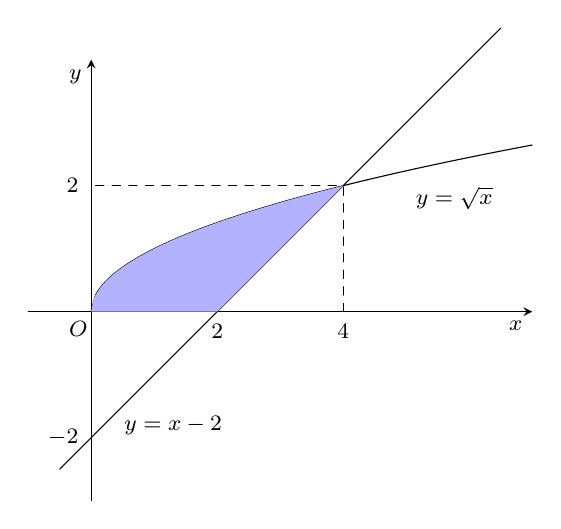
\begin{tikzpicture}[scale=.8, font=\footnotesize, line join=round, line cap=round, >=stealth]
		\draw[-stealth] (-1,0)--(7,0) node[below left]{$x$};
		\draw[-stealth] (0,-3)--(0,4) node[below left]{$y$};
		\draw[smooth,samples=100,domain=0:7] plot(\x,{sqrt{(\x)}});
		\draw[smooth,domain=-0.5:6.5] plot(\x,{\x-2})
		(0.1,0)node[below left]{$O$}
		(1.3,-1.5)node[below]{$y=x-2$}
		(5,1.8)node[right]{$y=\sqrt{x}$}
		;
		\fill[blue!30,smooth,samples=100] 
		plot[domain=0:4] (\x,{sqrt{(\x)}})--
		plot[domain=4:2] (\x,{(\x)-2})--
		plot[domain=2:0] (\x,{0})--cycle;
		\foreach \x in {2,4}
		\draw (\x,0.05)  ++(0,-0.1) node [below] {$\x$};
		\foreach \y in {-2,2} 
		\draw (0.05,\y)  ++(-0.1,0) node [left] {$\y$};
		\draw [dashed] (4,0)|-(0,2);
		\end{tikzpicture}
	}
	\loigiai{
		Áp dụng công thức tính thể tích: $V=\pi\displaystyle\int\limits_a^b \left|f^2(x)-g^2(x)\right|\mathrm{\,d}x$ ta có $V=\pi\left[\displaystyle\int\limits_0^4 x\mathrm{\,d}x-\displaystyle\int\limits_0^4(x-2)^2\mathrm{\,d}x\right]$.}
\end{ex}
\begin{ex}%Câu 15.%[Paul Hieu Nguyen]%[2D3Y3-3]
	Tính thể tích của vật thể tròn xoay khi quay hình $\mathscr H$ quanh $Ox$ với $\mathscr H$ được giới hạn bởi đồ thị hàm số $y=\sqrt{4x-x^2}$ và trục hoành.
	\choice
	{$\dfrac{35\pi}{3}$}
	{$\dfrac{31\pi}{3}$}
	{\True $\dfrac{32\pi}{3}$}
	{$\dfrac{34\pi}{3}$}
	\loigiai{
		Phương trình hoành độ giao điểm là $\sqrt{4x-x^2}=0\Leftrightarrow \hoac{&x=0\\&x=4.}$\\
		Ta có $x\in(0;4)\Rightarrow \sqrt{4x-x^2}>0$.\\
		Suy ra thể tích cần tính bằng $V=\pi\displaystyle\int\limits_0^4 \left(\sqrt{4x-x^2}\right)^2\mathrm{\,d}x=\dfrac{32\pi}{3}$.}
\end{ex}
\begin{ex}%Câu 16.%[Paul Hieu Nguyen]%[2D3Y3-3]
	Cho hình phẳng $\mathscr H$ giới hạn bởi các đường $y=\sin x$, $y=0$, $x=0$ và $x=5$. Tính thể tích vật thể tròn xoay sinh bởi hình phẳng $\mathscr H$ quay quanh trục $Ox$. 
	\choice
	{$\dfrac{\pi}{2}$}
	{\True $\dfrac{\pi^2}{2}$}
	{$\dfrac{\pi^2}{4}$}
	{$\dfrac{\pi}{4}$}
	\loigiai{
		Thể tích cần tính là $V=\pi\displaystyle\int\limits_0^\pi \sin^2x\mathrm{\,d}x=\dfrac{\pi^2}{2}$.}
\end{ex}
\begin{ex}%Câu 17.%[Paul Hieu Nguyen]%[2D3K3-3]
	Tính thể tích khối tròn xoay tạo thành khi quay elip $\dfrac{x^2}{3}+\dfrac{y^2}{b^2}=1$ quanh trục $Ox$.
	\choice
	{$4\pi b$}
	{$\dfrac{2\sqrt{3}}{3}\pi b^2$}
	{$\dfrac{4\sqrt{3}}{3}\pi b^2$}
	{\True $\dfrac{4\sqrt{3}}{6}\pi b^2$}
	\loigiai{
		Hình elip trên nhận $Ox$ làm trục đối xứng nên khối elip tròn xoay được sinh ra bởi nửa phía trên $Ox$ của elip khi quay quanh $Ox$.\\
		Phương trình nửa trên của elip $\dfrac{x^2}{3}+\dfrac{y^2}{b^2}=1$ là $y=\sqrt{b^2\left(1-\dfrac{x^2}{3}\right)}$.\\
		Khi đó $V=2\pi\displaystyle\int\limits_0^{\sqrt{3}} b^2\left(1-\dfrac{x^2}{3}\right) \mathrm{\,d}x=\dfrac{4}{3}\pi b^2\cdot\sqrt{3}=\dfrac{4\sqrt{3}}{3}\pi b^2$.}
\end{ex}
\begin{ex}%Câu 18.%[Paul Hieu Nguyen]%[2D3K3-3]
	Cho hình phẳng giới hạn bởi các đường $y=x\ln x$, $y=0$, $x=e$ quay xung quanh trục $Ox$ tạo thành khối tròn xoay có thể tích bằng $\dfrac{\pi}{a}\left(b\mathrm{e}^3-2\right)$. Tìm $a$ và $b$.
	\choice
	{\True $a=27$; $b=5$}
	{$a=26$; $b=6$}
	{$a=24$; $b=5$}
	{$a=27$; $b=6$}
	\loigiai{
		Phương pháp: Áp dụng công thức tính thể tích khối tròn xoay khi quay hình phẳng giới hạn bởi.\\
		$y=f(x)$, $y=0$, $x=a$, $x=b$ quanh trục $Ox$ là $V=\pi\displaystyle\int\limits_a^b f^2(x) \mathrm{\,d}x$.\\
		Xét phương trình: $x\ln x=0\Leftrightarrow\heva{&x>0\\&x=1}\Leftrightarrow x=1$.\\
		Áp dụng công thức trên ta có:\\
		$V=\pi\displaystyle\int\limits_1^e(x\ln x)^2\mathrm{\,d}x=\dfrac{1}{3}x^3\ln^2x\bigg|^e_1-\dfrac{2}{3}\displaystyle\int\limits_1^e x^2\ln x\mathrm{\,d}x=\dfrac{1}{3}\mathrm{e}^3-\left(\dfrac{2}{3}\mathrm{e}^3+\dfrac{1}{9}\right)=\left(5\mathrm{e}^3-2\right)\dfrac{\pi}{27}$.\\
		Do đó $a=27$, $b=5$.}
\end{ex}
\begin{ex}%Câu 19.%[Paul Hieu Nguyen]%[2D3K3-3]
	Gọi $V$ là thể tích của khối tròn xoay tạo thành khi quay quanh trục $Ox$ một Elip có phương trình $\dfrac{x^2}{9}+\dfrac{y^2}{4}=1$. Khi đó $V$ có giá trị gần nhất với giá trị nào sau đây?
	\choice
	{$60$}
	{$500$}
	{$10$}
	{\True $50$}
	\loigiai{
		$\dfrac{x^2}{9}+\dfrac{y^2}{4}=1\Leftrightarrow y^2=\dfrac{36-4x^2}{9}\Leftrightarrow y=\pm\sqrt{\dfrac{36-4x^2}{9}}=\pm\dfrac{\sqrt{36-4x^2}}{3}$.\\
		$V$ là thể tích của khối tròn xoay tạo thành khi quay quanh trục $Ox$ phần hình phẳng giới hạn bởi $y=\dfrac{\sqrt{36-4x^2}}{3}$ và trục hoành.\\
		Ta có $V=\pi\displaystyle\int\limits_{-3}^3\dfrac{36-4x^2}{9}\mathrm{\,d}x\approx 50{,}24$.}
\end{ex}
\begin{ex}%Câu 20.%[Paul Hieu Nguyen]%[2D3K3-3]
	Cho mặt phẳng $(H)$ giới hạn bởi các đường $y=\sqrt{\ln x}$, $y=0$, $x=1$ và $x=k$ $(k>1)$. Gọi $V_h$ là thể tích của khối tròn xoay thu được khi quay hình $(H)$ quay trục $Ox$. Biết rằng $V_h=\pi$, hãy chọn khẳng định đúng?
	\choice
	{$4<k<5$}
	{$3<k<4$}
	{$1<k<2$}
	{\True $2<k<3$}
	\loigiai{
		Ta có: $V_h=\pi\displaystyle\int\limits_1^k\ln x\mathrm{\,d}x$. Đặt $\heva{&u=\ln x\\&\mathrm{\,d}v=\mathrm{\,d}x}\Rightarrow\heva{&\mathrm{\,d}u=\dfrac{\mathrm{\,d}x}{x}\\&v=x.}$\\
		$\Rightarrow V_h=\pi\left(x\ln x\bigg|^k_1-\displaystyle\int\limits_1^k\mathrm{\,d}x\right)=\pi\left(x\ln x\bigg|^k_1-x\bigg|^k_1\right)$.\\
		$\Leftrightarrow V_h=\pi\left(x\ln x\bigg|^k_1-x\bigg|^k_1\right)=\pi(k\ln k-k+1)\Rightarrow k\ln k-k+1=1$\\
		$\Leftrightarrow k(\ln k-1)=0\Leftrightarrow\ln k-1=0\Leftrightarrow k=\mathrm{e}$\\
		$\Rightarrow 2<k<3$.}
\end{ex}
\begin{ex}%Câu 21.%[Paul Hieu Nguyen]%[2D3K3-3]
	\immini{
		Cho hình thang cong $(H)$ giới hạn bởi các đường $y=\dfrac{1}{x}$, $y=0$, $x=1$, $x=5$. Đường thẳng $x=k$ $(1<k<5)$ chia $(H)$ thành hai phần là $(S_1)$ và $(S_2)$ quay quanh trục $Ox$ ta thu được hai khối tròn xoay có thể tích lần lượt là $V_1$ và $V_2$. Xác định $k$ để $V_1=2V_2$.
		\choice
		{$k=\dfrac{5}{3}$}
		{\True $k=\dfrac{15}{7}$}
		{$k=\ln 5$}
		{$k=\sqrt[3]{25}$}
	}
	{
		\begin{tikzpicture}[scale=1, font=\footnotesize, line join=round, line cap=round, >=stealth, yscale=1.2]
		\draw[-stealth] (-1,0)--(6,0) node[below left]{$x$};
		\draw[-stealth] (0,-1)--(0,3) node[below left]{$y$};
		\draw[smooth,samples=100,domain=0.34:6] plot(\x,{1/(\x)});
		\draw plot[domain=-1:3] (1,\x)
		plot[domain=-1:3] (2.5,\x)
		plot[domain=-1:3] (5,\x)
		(0.1,0)node[below left]{$O$}
		(3,0.7)node[right]{$y=\frac{1}{x}$}
		(1.5,0)node[above]{$(S_1)$}
		(2.5,0.15)node[right]{$(S_2)$}
		;
		\fill[pattern=north east lines,smooth,samples=100] plot[domain=1:2.5] (\x,{1/(\x)})--plot[domain=2.5:1] (\x,{0});
		\fill[pattern=north west lines,smooth,samples=100] plot[domain=2.5:5] (\x,{1/(\x)})-- plot[domain=5:2.5] (\x,{0});
		\foreach \x in {1,5}
		\draw (\x,0.05)  ++(0,-0.1) node [below left] {$\x$};
		\draw (2.5,0) node [below left] {$k$};
		\end{tikzpicture}
	}
	\loigiai{
		Ta có: $\displaystyle\int\dfrac{\mathrm{\,d}x}{x^2}=-\dfrac{1}{x}=F(x)\Rightarrow\dfrac{V_1}{V_2}=\dfrac{\pi{\displaystyle\int\limits_1^k\left(\dfrac{1}{x}\right)}^2\mathrm{\,d}x}{\pi{\displaystyle\int\limits_k^5\left(\dfrac{1}{x}\right)}^2\mathrm{\,d}x}=\dfrac{F(k)-F(1)}{F(5)-F(k)}=2\Rightarrow k=\dfrac{15}{7}$.}
\end{ex}
\begin{ex}%Câu 22.%[Paul Hieu Nguyen]%[2D3B3-3]
	Trong mặt phẳng tọa độ $Oxy$, cho hình thang $ABCD$ với $A(-1;2)$, $B(5;5)$, $C(5;0)$, $D(-1;0)$. Quay hình thang $ABCD$ xung quanh trục $Ox$ thì thể tích khối nón tròn xoay tạo thành là bao nhiêu?
	\choice
	{$72\pi$}
	{$74\pi$}
	{$76\pi$}
	{\True $78\pi$}
	\loigiai{
		\immini{
			Thể tích cần tính là thể tích khối tròn xoay tạo bởi hình thang $ABCD$ giới hạn bởi các đường $y=\dfrac{x}{2}+\dfrac{5}{2}$; $y=0$; $x=-1$; $x=5$ (như hình vẽ).\\
			Khi đó: $V=\pi\displaystyle\int\limits_{-1}^5\left(\dfrac{x}{2}+\dfrac{5}{2}\right)^2\mathrm{\,d}x=78\pi$.}
		{
			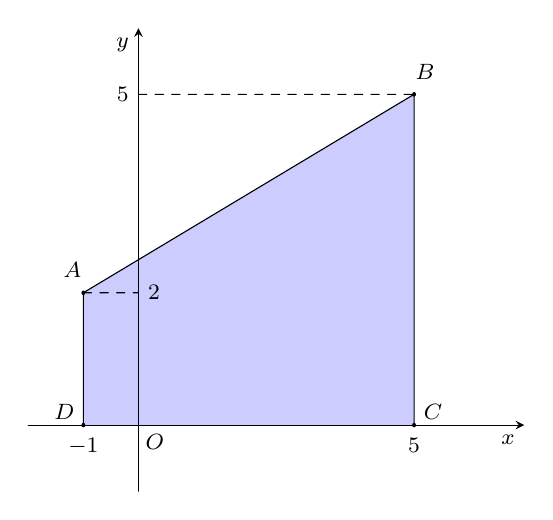
\begin{tikzpicture}[scale=.7, font=\footnotesize, line join=round, line cap=round, >=stealth, yscale=1.2]
			\coordinate (A) at (-1,2);
			\coordinate (B) at (5,5);
			\coordinate (C) at (5,0);
			\coordinate (D) at (-1,0);
			\draw[fill=blue!20] (D)--(A)--(B)--(C)
			(0.3,0)node[below]{$O$}
			(0,5)node[left]{$5$}
			(0,2)node[right]{$2$}
			;
			\draw[-stealth] (-2,0)--(7,0) node[below left]{$x$};
			\draw[-stealth] (0,-1)--(0,6) node[below left]{$y$};
			\draw[dashed] (0,5)--(B) (A)--(0,2);
			\foreach \d/\g in {A/120,B/60,C/30,D/150}
			\fill[black](\d) circle (1pt)+(\g:.4)node{$\d$};
			\foreach \x in {-1,5}
			\draw (\x,0.05)  ++(0,-0.1) node [below] {$\x$};
			\end{tikzpicture}
		}
	}
\end{ex}
\begin{ex}%Câu 23.%[Paul Hieu Nguyen]%[2D3K3-3]
	Goi $V$ là thể tích vật tròn xoay khi quay hình phẳng giới hạn bởi đồ thị hàm số $y=\sqrt{\dfrac{\ln x}{x(\ln x+1)^2}}$, trục $Ox$, đường thẳng $x=\mathrm{e}$ quanh trục $Ox$. Biết $V=\pi(a\ln 2+b)$ với $a$, $b\in\mathbb{Q}$. Khẳng định nào sau đây là đúng?
	\choice
	{\True $a+2b=0$}
	{$a^2+b^2=4$}
	{$a-b=1$}
	{$ab=2$}
	\loigiai{
		Thể tích khối tròn xoay là\\
		$V=\pi\displaystyle\int\limits_1^\mathrm{e}\dfrac{\ln x}{x(\ln x+1)^2}\mathrm{\,d}x$. 
		Đặt $t=\ln x+1\Rightarrow \mathrm{\,d}t=\dfrac{1}{x}\mathrm{\,d}x$.\\
		Khi đó $V=\pi\displaystyle\int\limits_1^2\dfrac{t-1}{t^2}\mathrm{\,d}t=\pi\left(\ln 2-\dfrac{1}{2}\right)$.\\
		Suy ra $a=1$; $b=-\dfrac{1}{2}\Rightarrow a+2b=0$.}
\end{ex}
\begin{ex}%Câu 24.%[Paul Hieu Nguyen]%[2D3B3-3]
	Cho hàm số $y=4-x^4$ có đồ thị $(C)$, khối tròn xoay tạo thành khi quay hình phẳng giới hạn bởi $(C)$ và trục $Ox$, quanh trục $Oy$ có thể tích là 
	\choice
	{$V=\dfrac{32\pi}{3}$}
	{\True $V=\dfrac{16\pi}{3}$}
	{$V=\dfrac{1024\sqrt{2}\pi}{45}$}
	{$V=\dfrac{\left(16-2(4-\sqrt{2})^{\tfrac{3}{2}}\right)\pi}{3}$}
	\loigiai{
		\immini{
			Do tính đối xứng nên thể tích cần tìm bằng thể tích khối tròn xoay tạo thành khi quay hình phẳng giới hạn bởi đường cong $x=\sqrt[4]{4-y}$, trục $Oy$ và hai đường thẳng $y=0$, $y=4$ quanh trục $Oy$.\\
			$V=\pi\displaystyle\int\limits_0^4\sqrt{4-y} dy=\pi\displaystyle\int\limits_0^4(4-y)^{\tfrac{1}{2}}dy=-\dfrac{2\pi}{3}(4-y)^{\tfrac{3}{2}}\bigg|_0^4=\dfrac{16\pi}{3}$.}
		{
			\begin{tikzpicture}[scale=.8, font=\footnotesize, line join=round, line cap=round, >=stealth]
			\draw[-stealth] (-3,0)--(3,0) node[below left]{$x$};
			\draw[-stealth] (0,-2)--(0,5.5) node[below right]{$y$};
			\draw[smooth,samples=100,domain=-1.5:1.5] plot(\x,{4-(\x)^4})
			(0.3,0)node[below]{$O$}
			(0,4)node[above left]{$4$}
			(1.3,2)node[right]{$(C)$}
			%(1.3,0.3)node[right]{$\sqrt{2}$}
			%(-1.3,0.3)node[left]{$-\sqrt{2}$}
			;
			\foreach \x in {-2,-1,1,2}
			\draw (\x,0.05)  ++(0,-0.1) node [below] {$\x$};
			\foreach \x in {-2,...,2}
			\draw (\x,0.05)--++(0,-0.1);
			\foreach \y in {-1,...,4} 
			\draw (0.05,\y)--++(-0.1,0);
			\end{tikzpicture}
		}
	}
\end{ex}
\begin{ex}%Câu 25.%[Paul Hieu Nguyen]%[2D3G3-5]
	\immini{
		Có một vật thể là hình tròn xoay có dạng giống như một cái ly như hình vẽ bên. Người ta đo được đường kính của miệng ly là $4$cm và chiều cao là $6$cm. Biết rằng thiết diện của chiếc ly cắt bởi mặt phẳng qua trục đối xứng là một Parabol. Tính thể tích $V$ (cm$^3$) của vật thể đã cho.
		\choice
		{$V=\dfrac{72\pi}{5}$}
		{$V=12$}
		{\True $V=12\pi$}
		{$V=\dfrac{72}{5}$}
	}
	{
		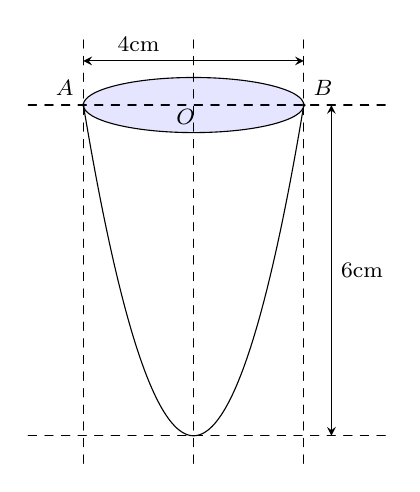
\begin{tikzpicture}[scale=.7, font=\footnotesize, line join=round, line cap=round, >=stealth]
		\draw[fill=blue!10] (2,0) arc (0:360:2 cm and .5 cm);
		\draw[dashed] (-3,0)--(3.5,0) (0,-6.5)--(0,1.3)
		(-3,-6)--(3.5,-6) (-2,-6.5)--(-2,1.3) (2,-6.5)--(2,1.3);
		\draw[<->] (-2,.8)--(2,.8) node[near start,above] {$4$cm};
		\draw[<->] (2.5,0)--(2.5,-6) node[midway,right] {$6$cm};
		\draw[smooth,samples=100,domain=-2:2] plot(\x,{(3/2)*(\x)^2-6})
		(0.2,0.1)node[below left]{$O$}
		;
		\fill[black](-2,0) circle (1pt) node[above left]{$A$};
		\fill[black](2,0) circle (1pt) node[above right]{$B$};
		\end{tikzpicture}
	}
	\loigiai{
		\immini{
			Chọn hệ trục tọa độ $Oxy$ như hình vẽ.\\
			Parabol có đỉnh $(0;-6)$ và đi qua các điểm $(-2;0)$ và $(2;0)$ nên có phương trình $y=\dfrac{3}{2}x^2-6$.\\
			Thể tích của vật là thể tích khối tròn xoay khi quay hình $(H)$ giới hạn bởi các đường $x=\sqrt{\dfrac{2y+12}{3}}$, $x=0$, $y=-6$, $y=0$ quanh trục tung.\\
			Khi đó $V=\pi\displaystyle\int\limits_{-6}^0\dfrac{2y+12}{3}dy=\pi\left(\dfrac{1}{3}y^2+4y\right)\bigg|_{-6}^0=12\pi$.
		}
		{
			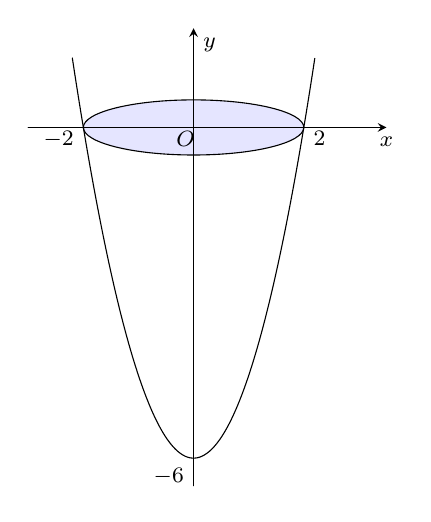
\begin{tikzpicture}[scale=.7, font=\footnotesize, line join=round, line cap=round, >=stealth]
			\draw[fill=blue!10] (2,0) arc (0:360:2 cm and .5 cm);
			\draw[-stealth] (-3,0)--(3.5,0) node[below]{$x$};
			\draw[-stealth] (0,-6.5)--(0,1.8) node[below right]{$y$};
			\draw[smooth,samples=100,domain=-2.2:2.2] plot(\x,{(3/2)*(\x)^2-6})
			(0.2,0.1)node[below left]{$O$}
			(-2,0.1)node[below left]{$-2$}
			(2,0.1)node[below right]{$2$}
			(0,-6)node[below left]{$-6$}
			;
			\end{tikzpicture}
		}
	}
\end{ex}
\begin{ex}%Câu 26.%[Paul Hieu Nguyen]%[2D3K3-3]
	\immini{
		Cho hai đường tròn $(O_1;5)$ và $(O_2;3)$ cắt nhau tại $2$ điểm $A$, $B$ sao cho $AB$ là một đường kính của đường tròn $(O_2)$. Gọi $(D)$ là hình thẳng được giới hạn bởi hai đường tròn (ở ngoài đường tròn lớn, phần được gạch chéo như hình vẽ). Quay $(D)$ quanh trục $O_1O_2$ ta được một khối tròn xoay. Tính thể tích khối tròn xoay được tạo thành.
		\choice
		{$V=\dfrac{14\pi}{3}$}
		{$V=\dfrac{68\pi}{3}$}
		{\True $V=\dfrac{40\pi}{3}$}
		{$V=36\pi$}
	}
	{
		\begin{tikzpicture}[scale=.7, font=\footnotesize, line join=round, line cap=round, >=stealth, xscale=.7, yscale=.7]
		\fill[pattern=north east lines,smooth,samples=100] (4,0) circle (3 cm);
		\draw[fill=white] (0,0) circle (5 cm);
		\draw (4,0) circle (3 cm);
		\draw (-5,0)--(7,0);
		\draw	
		(0,0)node[below]{$O_1$} circle (1pt)
		(4,0)node[below left]{$O_2$} circle (1pt)
		(5.8,1.2)node{$(D)$}
		;
		\draw[fill=black] (4,3) node[above]{$A$} circle (1pt)--(4,-3) node[below]{$B$} circle (1pt);
		\end{tikzpicture}
	}
	\loigiai{
		\immini{
			Gọi $V_1$ là thể tích của khối tròn xoay sinh ra khi quay hình phẳng $D_1$ được giới hạn bởi các đường $y=\sqrt{9-(x-4)^2}$, $y=0$, $x=4$, $x=7$ quay trục tung $\Rightarrow V_1=\pi\displaystyle\int\limits_4^7\left[9-(x-4)^2\right]\mathrm{\,d}x$.\\
			Gọi $V_2$ là thể tích khối tròn xoay sinh ra khi quay hình phẳng $D_2$ được giới hạn bởi các đường $y=\sqrt{25-x^2}$, $y=0$, $x=4$, $x=5$ quay trục tung $\Rightarrow V_2=\pi\displaystyle\int\limits_4^5\left(25-x^2\right)\mathrm{\,d}x$. \\
			Khi đó thể tích khối tròn xoay cần tính là $$V=V_1-V_2=\pi\displaystyle\int\limits_4^7\left[9-(x-4)^2\right]\mathrm{\,d}x-\pi\displaystyle\int\limits_4^5\left(25-x^2\right)\mathrm{\,d}x.$$
			Suy ra $V=\dfrac{40}{3}\pi$.}
		{
			\begin{tikzpicture}[scale=.7, font=\footnotesize, line join=round, line cap=round, >=stealth, xscale=.7, yscale=.7]
			\draw[-stealth] (-5.5,0)--(8,0) node[below]{$x$};
			\draw[-stealth] (0,-5.5)--(0,6) node[below right]{$y$};
			\draw (0,0) circle (5 cm) (4,0) circle (3 cm);
			\draw	
			(0.2,0.1)node[below left]{$O$}
			(4.1,0)node[below left]{$4$}
			(4.9,0)node[below right]{$5$}
			(6.8,0)node[below right]{$7$}
			(3.5,.5)node[above]{$D_2$}
			(6.5,2)node[above]{$D_1$}
			;
			\draw[fill=black] (4,3) circle (1pt)--(4,-3) circle (1pt);
			
			\fill[pattern=north west lines,smooth,samples=100] 
			plot[domain=4:5] (\x,{sqrt(25-(\x)^2)})--
			plot[domain=5:4] (\x,{0})
			;
			\fill[pattern=north east lines,smooth,samples=100] 
			plot[domain=4:7] (\x,{sqrt(9-(\x-4)^2)})--
			plot[domain=7:4] (\x,{0})
			;
			\end{tikzpicture}
		}
	}
\end{ex}
\begin{ex}%Câu 27:%[Paul Hieu Nguyen]%[2D3K3-3]
	\immini{
		Gọi $V$ là thể tích khối tròn xoay tạo thành khi quay hình phẳng giới hạn bởi các đường $y=\sqrt{x}$, $y=0$ và $x=4$ quanh trục $Ox$. Đường thẳng $x=a$ $(0<a<4)$ cắt đồ thị hàm $y=\sqrt{x}$ tại $M$ (hình vẽ bên). Gọi $V_1$ là thể tích khối tròn xoay tạo thành khi quay tam giác $OMH$ quanh trục $Ox$. Biết rằng $V=2V_1$. Khi đó
		\choice
		{$a=2$}
		{$a=2\sqrt{2}$}
		{$a=\dfrac{5}{2}$}
		{\True $a=3$}
	}
	{
		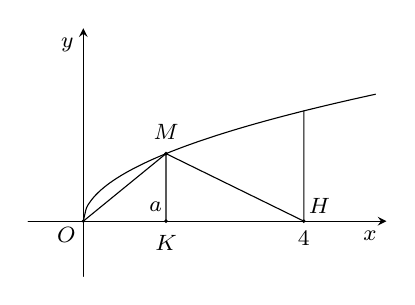
\begin{tikzpicture}[scale=.7, font=\footnotesize, line join=round, line cap=round, >=stealth]
		\coordinate (O) at (0,0);
		\coordinate (M) at (1.5,1.2247);
		\coordinate (K) at (1.5,0);
		\coordinate (I) at (4,2);
		\coordinate (H) at (4,0);
		\draw (O)--(M)--(K) (M)--(H)--(I);
		\draw[-stealth] (-1,0)--(5.5,0) node[below left]{$x$};
		\draw[-stealth] (0,-1)--(0,3.5) node[below left]{$y$};
		\foreach \d/\g in {O/220,M/90,K/-90,H/45}
		\fill[black](\d) circle (1pt)+(\g:.4)node{$\d$};
		\draw[smooth,samples=100,domain=0:5.3] plot(\x,{sqrt{(\x)}})
		(4,0)node[below]{$4$}
		(1.6,0)node[above left]{$a$}
		;
		\end{tikzpicture}
	}
	\loigiai{
		Ta có $\sqrt{x}=0\Leftrightarrow x=0$. Khi đó $V=\pi\displaystyle\int\limits_0^4 x\mathrm{\,d}x=8\pi$.\\
		Ta có $M(a;\sqrt{a})$.\\
		Khi quay tam giác $OMH$ quanh trục $Ox$ tạo thành hai hình nón có chung đáy:\\
		Hình nón $(N_1)$ có đỉnh là $O$, chiều cao $h=OK=a$, bán kính đáy $R=MK=\sqrt{a}$;\\
		hình nón $(N_2)$ có đỉnh là $H$, chiều cao $h_2=HK=4-a$, bán kính đáy $R=MK=\sqrt{a}$.\\
		Khi đó $V_1=\dfrac{1}{3}\pi R^2h_1+\dfrac{1}{3}\pi R^2h_2=\dfrac{4}{3}\pi$.\\
		Theo đề bài $V=2V_1\Leftrightarrow 8\pi=2\cdot\dfrac{4}{3}\pi a \Rightarrow a=3$.}
\end{ex}
\begin{ex}%Câu 28.%[Paul Hieu Nguyen]%[2D3K3-3]
	\immini{
		Một khối cầu có bán kính $5$dm, người ta cắt bỏ $2$ phần bằng hai mặt phẳng vuông góc bán kính và cách tâm $3$dm để làm một chiếc lu đựng. Tính thể tích mà chiếc lu chứa được. 
		\choice
		{\True $132\pi$ (dm$^3$)}
		{$41\pi$ (dm$^3$)}
		{$\dfrac{100}{3}\pi$ (dm$^3$)}
		{$43\pi$ (dm$^3$)}
	}
	{
		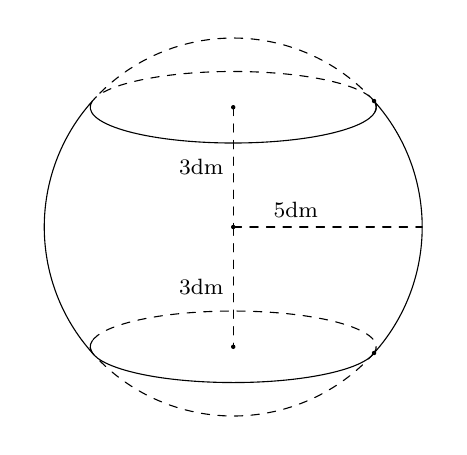
\begin{tikzpicture}[scale=.8, font=\footnotesize, line join=round, line cap=round, >=stealth]
		\def\r{3}
		\def\h{2}
		\def\g{10}
		\pgfmathsetmacro{\a}{sqrt((\r)^2-(\h)^2)*sec(\g)}
		\pgfmathsetmacro{\b}{\a/4}
		\pgfmathsetmacro{\bm}{\b *sin(\g)}
		\pgfmathsetmacro{\gm}{asin(\h/\r)}
		\path (0:0) coordinate (I)
		(270:\h-\bm) coordinate (J)
		(-\gm:\r) coordinate (M)
		(\gm:\r) coordinate (N)
		(0:\r) coordinate (E)
		(90:\h-\bm) coordinate (K)
		;
		\draw[dashed] (M) arc(-\gm:-180+\gm:\r) 
		arc (180+\g:-\g:{\a} and {\b});
		\draw[dashed] (N) arc(\gm:180-\gm:\r)
		arc (180-\g:-\g:{\a} and {\b});
		\draw (M) arc(-\gm:\gm:\r) arc (\g:-180-\g:{\a} and {\b})
		arc(180-\gm:180+\gm:\r);
		\draw (M) arc(-\g:-180-\g:{\a} and {\b});
		\foreach \d in {I,J,M,N,K}
		\fill[black](\d) circle (1pt);
		\draw[dashed] (K)--(I) node[midway,left] {$3$dm}
		(I)--(J) node[midway,left] {$3$dm}
		(I)--(E) node[midway,above left] {$5$dm};
		\end{tikzpicture}	
	}
	\loigiai{
		Đặt hệ trục với tâm $O$, là tâm của mặt cầu; đường thẳng đứng là $Ox$, đường ngang là $Oy$; đường tròn lớn có phương trình $x^2+y^2=25$.\\
		Thể tích là do hình giới hạn bởi $Ox$, đường cong $y=\sqrt{25-x^2}$, $x=3$, $x=-3$ quay quanh $Ox$.\\
		$V=\pi\displaystyle\int\limits_{-3}^3\left(25-x^2\right)\mathrm{\,d}x =132\pi$.}
\end{ex}
\begin{ex}%Câu 29.%[Paul Hieu Nguyen]%[2D3K3-3]
	Trong hệ trục $Oxy$, cho tam giác $OAB$ vuông ở $A$, điểm $B$ nằm trong góc phần tư thứ nhất, $A$ nằm trên trục hoành, $OB=2017$. Góc $\widehat{AOB}=\alpha,\left(0<\alpha<\dfrac{\pi}{3}\right)$. Khi quay tam giác đó quanh trục $Ox$ ta được khối nón tròn xoay. Thể tích của khối nón lớn nhất khi
	\choice
	{\True $\sin\alpha=\dfrac{\sqrt{6}}{3}$}
	{$\cos\alpha=\dfrac{\sqrt{3}}{2}$}
	{$\cos\alpha=\dfrac{1}{2}$}
	{$\sin\alpha=\dfrac{\sqrt{2}}{3}$}
	\loigiai{
		PTĐT $OB\colon y=x\cdot\tan\alpha$; $OA=2017\cos\alpha$.\\
		Khi đó thể tích nón tròn xoay là $$V=\pi\displaystyle\int\limits_0^{2017\cdot \cos\alpha} x^2\tan^2\alpha\cdot \mathrm{\,d}x=\dfrac{{2017}^3\cdot\pi}{3}\cdot \cos\alpha\cdot \sin^2\alpha=\dfrac{{2017}^3\cdot\pi}{3}\cdot \cos\alpha\left(1-\cos^2\alpha\right).$$
		Đặt $t=\cos\alpha\Rightarrow t\in\left(0;\dfrac{1}{2}\right)$. Xét hàm số $f(t)=t\left(1-t^2\right)$, $t\in\left(0;\dfrac{1}{2}\right)$.\\
		Ta tìm được $f(t)$ lớn nhất khi $t=\dfrac{\sqrt{3}}{3}\Rightarrow\cos\alpha=\dfrac{\sqrt{3}}{3}\Rightarrow\sin\alpha=\dfrac{\sqrt{6}}{3}$.}
\end{ex}
\Closesolutionfile{ans}
% \DAPAN
\inputansbox{10}{ans/BAI-3-DANG-1}

\Opensolutionfile{ans}[ans/2D3-3.2]
\begin{dang}{Thể tích khối tròn xoay sinh bởi hình phẳng giới hạn bởi các đường $y=f(x),y=g(x), x=a, x=b$ khi quay quanh trục $Ox$ được tính bởi công thức: $V=\pi\displaystyle\int\limits_a^b |f^2(x)-g^2(x)| \mathrm{\,d}x$}.
\end{dang}
\subsubsection{Các ví dụ}
\begin{vd}%Ví dụ 1.%[DuongPham - ĐCHT THPT]%[2D3Y3-3]
	Thể tích của khối tròn xoay khi cho hình phẳng giới hạn bởi Parabol $(P)\colon y=2x^2$ và đường thẳng $d\colon y=x$ quay xung quanh trục $Ox$ được tính bởi công thức nào dưới đây?
	\choice
	{\True $V=\pi\displaystyle\int\limits_0^{\tfrac{1}{2}} x^2\mathrm{\,d}x-4\pi\displaystyle\int\limits_0^{\tfrac{1}{2}} x^4\mathrm{\,d}x$}
	{$V=\pi\displaystyle\int\limits_0^{\tfrac{1}{2}}\left(x-2x^2\right)\mathrm{\,d}x$}
	{$V=\pi\displaystyle\int\limits_0^{\tfrac{1}{2}}\left(2x^2-x\right)^2\mathrm{\,d}x$}
	{$V=\pi\displaystyle\int\limits_0^{\tfrac{1}{2}} x^2\mathrm{\,d}x+4\pi\displaystyle\int\limits_0^{\tfrac{1}{2}} x^4\mathrm{\,d}x$}
	\loigiai{
		Phương trình hoành độ giao điểm của $(P)$ và $(d)$ là $2x^2=x\Leftrightarrow x(2x-1)=0\Leftrightarrow\hoac{&x=0\\&x=\dfrac{1}{2}.}$ \\
		Thể tích của khối tròn xoay cần tính là $V=\pi\displaystyle\int\limits_0^{\tfrac{1}{2}} x^2\mathrm{\,d}x-4\pi\displaystyle\int\limits_0^{\tfrac{1}{2}} x^4\mathrm{\,d}x$.}
\end{vd}
\begin{vd}%Ví dụ 2.%[DuongPham - ĐCHT THPT]%[2D3B3-3]
	Cho hình phẳng $D$ giới hạn bởi các đường
	$y=\left|x^2-4x+3\right|;y=x+3$. Cho hình phẳng $D$ quay quanh trục $Ox$. Tính thể tích khối tròn xoay tạo thành. 
	\choice
	{$120\pi$ (đvtt)}
	{$100\pi$ (đvtt)}
	{\True $125\pi$ (đvtt)}
	{$115\pi$ (đvtt)}
	\loigiai{
		Phương pháp: Cho hàm số $y=f(x)$ và $y=g(x)$ liên tục trên $[a;b]$ Khi đó thể
		tích khối tròn xoay giới hạn bởi hai đồ thị hàm số trên và hai đường thẳng $x=a,y=b$ quay
		quanh trục $Ox$ là $V=\pi\displaystyle\int\limits_a^b\left|f^2(x)-g^2(x)\right|\mathrm{\,d}x$.\\
		Ta có: $\left|x^2-4x+3\right|=x+3\Leftrightarrow\hoac{&x^2-4x+3=x+3\\&x^2-4x+3=-x-3}\Rightarrow\hoac{&x=0\\&x=5.}$ \\
		Vậy thể tích khối tròn xoay là $V=\pi\displaystyle\int\limits_0^5\left|\left|x^2-4x+ 3\right|^2-(x+3)^2\right|\mathrm{\,d}x=125\pi$ (đvtt).}
\end{vd}
\begin{vd}%Ví dụ 3.%[DuongPham - ĐCHT THPT]%[2D3B3-3]
	\immini{Quay hình phẳng $(H)$ như hình được tô đậm trong hình vẽ bên quanh trục $Ox$ ta được khối tròn xoay có thể tích là 
		\choice
		{\True $V=4\sqrt{3}\pi$}
		{$V=6\sqrt{3}\pi$}
		{$V=5\sqrt{3}\pi$}
		{$V=2\sqrt{3}\pi$}}{\begin{tikzpicture}[scale=0.8,>=stealth, font=\footnotesize, line join=round, line cap=round]
		\def\xmin{-3} \def\xmax{3}  \def\ymin{-3}  \def\ymax{3} 
		%	\draw[color=gray!50,dashed] (\xmin,\ymin) grid (\xmax,\ymax);
		\draw[->] (\xmin,0)--(\xmax,0) node [below]{$x$};
		\draw[->] (0,\ymin)--(0,\ymax) node [left]{$y$};
		\clip (\xmin,\ymin) rectangle (\xmax,\ymax);
		\def\f(#1){sqrt(4-(#1)^2)}
		%%%%
		\draw(0,0)circle(2) (\xmin,1)--(\xmax,1);
		\fill[pattern=crosshatch dots,smooth] (-2,1) --
		plot[domain=-sqrt(3):sqrt(3)] (\x,{\f(\x)})
		-- (2,1) -- cycle;
		\foreach \i in{-2,-1,1,2}\fill[black](\i,0)node[below right]{$\i$}circle(1pt);
		\draw[fill=black](0,0)node[below right]{$O$}circle(1pt) (0,1)node[below right]{$1$}circle(1pt) (1.75,1)node [above right]{$y=1$};
		\end{tikzpicture}}
	\loigiai{
		Xét hệ phương trình: $\heva{&x^2+y^2=4\\&y=1}\Leftrightarrow\heva{&x^2=3\\&y=1}\Rightarrow\hoac{&x=\sqrt{3}\\&x=-\sqrt{3}.}$\\
		Do (H) đối xứng nhau qua $Oy$ nên: 
		$V=2\pi\displaystyle\int\limits_0^{\sqrt{3}} \left[(4-x^2)-1^2\right] \mathrm{\,d}x=2\pi\displaystyle\int\limits_0^{\sqrt{3}} (3-x^2) \mathrm{\,d}x=4\sqrt{3}$.
	}
\end{vd}
\begin{vd}%Ví dụ 4.%[DuongPham - ĐCHT THPT]%[2D3K3-5]
	\immini{	Trong chương trình nông thôn mới, tại một xã X có xây một cây cầu bằng bê tông như hình vẽ. Tính thể tích khối bê tông để đổ đủ cây cầu (Đường cong trong hình vẽ là các đường Parabol)
		\choice
		{$19\,\mathrm{m^3}$}
		{$21\,\mathrm{m^3}$}
		{$18\,\mathrm{m^3}$}
		{\True $40\,\mathrm{m^3}$}}{\begin{tikzpicture}[>=stealth,scale=0.7]	
		\draw[  ] (-1,0)--(1,0)  ;
		\draw[ ] (0,0)--(0,2)  ;
		\draw plot[smooth,domain=-1:1] (\x,{-1.5*(\x)^2+1.5});
		\draw plot[smooth,domain=-1.5:1.5] (\x,{-(\x)^2+2.25});
		\coordinate (S) at (8,1);
		\draw[shift={(S)},dashed] plot[smooth,domain=-1:1] (\x,{-1.5*(\x)^2+1.5});
		\draw[shift={(S)}] plot[smooth,domain=0:1.5] (\x,{-(\x)^2+2.25});
		\draw[shift={(S)},dashed] plot[smooth,domain=-1.5:0] (\x,{-(\x)^2+2.25});
		\fill[opacity=.2] (0,2.25)--($(0,2.25)+(S)$)-- plot[shift={(S)},smooth,domain=0:1.5] (\x,{-(\x)^2+2.25})--(1.5,0)plot[smooth,domain=1.5:0] (\x,{-(\x)^2+2.25})--cycle;
		\draw[dashed] (-1.5,0)--($(-1.5,0)+(S)$)--($(1.5,0)+(S)$);
		\draw ($(1.5,0)+(S)$)--(1.5,0)node[pos=.5,below] {$5$ m};
		\draw [dashed] (0,1.5)--($(0,1.5)+(S)$) (0,0)--($(0,0)+(S)$) ;
		\draw (-1.5,0)--(-1,0) node[pos=.5,below] {\footnotesize$0.5$ m};
		\draw (1.5,0)--(1,0) node[pos=.5,below] {\footnotesize$0.5$ m};
		\draw (-1,0)--(1,0) node[pos=.5,below] {\footnotesize$19$ m};
		\draw (0,0)--(0,1.5) node[pos=.5,right] {\footnotesize$2$ m};
		\draw (0,1.5)--(0,2.25) node[pos=.5,right] {\footnotesize$0.5$ m};
		\end{tikzpicture}
	}
	\loigiai{
		\immini{
			Diện tích mặt cắt là diện tích phần gạch chéo như hình dưới đây.\\
			Parabol nằm trên có phương trình là $y=ax^2+\dfrac{5}{2}$ do $\heva{&x=10\\&y=0}\\\Rightarrow a=-\dfrac{1}{40}\Rightarrow y=\dfrac{-x^2}{40}+\dfrac{5}{2.}$ \\
			Tương tự: Parabol nằm dưới có phương trình là $y=\dfrac{-8}{361}x^2+2$.\\
			Khi đó $$\displaystyle\int\limits_{-10}^{10}\left(-\dfrac{x^2}{40}+\dfrac{5}{2}\right)\mathrm{\,d}x-\displaystyle\int\limits_{-9,5}^{9, 5}\left(-\dfrac{8}{361}x^2+2\right)\mathrm{\,d}x=8\Leftrightarrow V=8\cdot 5=40\,\mathrm{m^3}.$$}{\begin{tikzpicture}[scale=0.65]	
			\clip(- 5,- 5) rectangle (5.5, 5.5);
			\draw[->,line width = 1pt] (-5,0) --(0,0) node[below left]{$O$}--(4.5,0) node[below]{$x$};
			\draw[->,line width = 1pt] (0,-2) --(0,5) node[right]{$y$};
			\draw (0,4)  circle (1pt);
			\draw (0,4) node[above right]{$2.5$} circle (1pt);
			\draw (0,2)  circle (1pt);
			\draw (0,2) node[above right]{$2$} circle (1pt);
			\draw (4,0)  circle (1pt);
			\draw (- 4,0)  circle (1pt);
			\draw (4,0) node[below]{$10$} circle (1pt);
			\draw (- 4,0) node[below]{$-10$} circle (1pt);
			\draw (2,0)  circle (1pt);
			\draw (- 2,0)  circle (1pt);
			\draw (2,0) node[below]{$9.5$} circle (1pt);
			\draw (- 2,0) node[below]{$-9.5$} circle (1pt);
			
			\draw [samples=100, domain= - 4: 4] plot (\x, {(-0.25* (\x)^2) + 4});
			\draw [samples=100, domain= - 2: 2] plot (\x, {(-0.5* (\x)^2) + 2});
			\end{tikzpicture}}
	}
\end{vd}
\subsubsection{Câu hỏi trắc nghiệm}
\begin{ex}%Câu 29.%[DuongPham - ĐCHT THPT]%[2D3B3-3]
	Thể tích của khối tròn xoay khi cho hình phẳng giới hạn bởi Parabol $(P)\colon y=x^2$ và đường thẳng $d\colon y=2x$ quay xung quanh trục $Ox$ bằng 
	\choice
	{$\pi\displaystyle\int\limits_0^2\left(x^2-2x\right)^2\mathrm{\,d}x$}
	{$\pi\displaystyle\int\limits_0^2\left(2x-x^2\right)\mathrm{\,d}x$}
	{$\pi\displaystyle\int\limits_0^2 4 x^2\mathrm{\,d}x+\pi\displaystyle\int\limits_0^2 x^4\mathrm{\,d}x$}
	{\True $\pi\displaystyle\int\limits_0^2 4 x^2\mathrm{\,d}x-\pi\displaystyle\int\limits_0^2 x^4\mathrm{\,d}x$}
	\loigiai{
		Phương trình hoành độ giao điểm $x^2=2x\Leftrightarrow x=0$ hoặc $x=2$.\\
		Do $2x\geq x^2$ với $x\in (0;2)$ nên $V=V_1-V_2$ trong đó $V_1$ là thể tích khối tròn xoay khi cho hình phẳng giới hạn bởi đường thẳng $d\colon y=2x$, trục $Ox$, đường thẳng $x=2$ và trục $Ox$ quay quanh trục $Ox$; $V_2$ là thể tích khối tròn xoay khi cho hình phẳng giới hạn bởi Parabol
		$(P)$, trục $Ox$, đường thẳng $x=2$ và trục $Ox$ quay quanh trục $Ox$.
	}
\end{ex}
\begin{ex}%Câu 30.%[DuongPham - ĐCHT THPT]%[2D3B3-3]
	Cho hình phẳng $(H)$ giới hạn bởi các đường $y=x^2$ và $y=\sqrt{x}$. Khối tròn xoay tạo ra khi $(H)$ quay quanh $Ox$ có thể tích là 
	\choice
	{$\pi\displaystyle\int\limits_0^1\left(x^4-x\right)\mathrm{\,d}x\,\text{(đvtt)}$}
	{$\pi\displaystyle\int\limits_0^1\left(x^2-\sqrt{x}\right)\mathrm{\,d}x\,\text{(đvtt)}$}
	{$\pi\displaystyle\int\limits_0^1\left(\sqrt{x}-x^2\right)\mathrm{\,d}x\,\text{(đvtt)}$}
	{\True $\pi\displaystyle\int\limits_0^1\left(x-x^4\right)\mathrm{\,d}x\,\text{(đvtt)}$}
	\loigiai{
		Xét phương trình hoành độ giao điểm $x^2=\sqrt{x}\Leftrightarrow\hoac{&x=0\\&x=1.}$\\ Suy ra $V=\pi\displaystyle\int\limits_0^1\left|(x^2)^2-(\sqrt{x})^2\right|\mathrm{\,d}x=\pi\displaystyle\int\limits_0^1\left|x^4-x\right|\mathrm{\,d}x=\pi\displaystyle\int\limits_0^1\left(x-x^4\right)\mathrm{\,d}x$.}
\end{ex}
\begin{ex}%Câu 31.%[DuongPham - ĐCHT THPT]%[2D3B3-3]
	Thể tích của khối tròn xoay khi cho hình phẳng giới hạn bởi Parabol $(P)\colon y=x^2$ và đường thẳng $(d)\colon y=x$ xoay quanh trục $Ox$ bằng 
	\choice
	{\True $\pi\displaystyle\int\limits_0^1 x^2\mathrm{\,d}x-\pi\displaystyle\int\limits_0^1 x^4\mathrm{\,d}x$}
	{$\pi\displaystyle\int\limits_0^1 x^2\mathrm{\,d}x+\pi\displaystyle\int\limits_0^1 x^4\mathrm{\,d}x$}
	{$\pi\displaystyle\int\limits_0^1\left(x^2-x\right)^2\mathrm{\,d}x$}
	{$\pi\displaystyle\int\limits_0^1\left(x^2-x\right)\mathrm{\,d}x$}
	\loigiai{
		Tìm cận:	
		Phương trình hoành độ giao điểm $x^2=x\Leftrightarrow\hoac{&x=0\\&x=1.}$ \\
		Thể tích cần tìm là	\\	$V=\pi\displaystyle\int\limits_0^1\left|x^4-x^2\right|\mathrm{\,d}x\Leftrightarrow V=\pi\displaystyle\int\limits_0^1\left(x^2-x^4\right)\mathrm{\,d}x$ vì $x^2-x^4\ge 0$ với $x$ thuộc $[0;1]$.}
\end{ex}
\begin{ex}%Câu 32.%[DuongPham - ĐCHT THPT]%[2D3B3-3]
	Tính thể tích khối tròn xoay khi cho hình phẳng giới hạn bởi đồ thị các hàm số $y=x^2-2x$ và $y=-x^2$ quay quanh trục $Ox$. 
	\choice
	{$\dfrac{4}{3}$}
	{$\dfrac{4\pi}{3}$}
	{\True $\dfrac{\pi}{3}$}
	{$\dfrac{1}{3}$}
	\loigiai{
		Xét $x^2-2x=-x^2\Rightarrow x=0; x=1$. $V_1=\pi\displaystyle\int\limits_0^1\left(x^2-2x\right)^2\mathrm{\,d}x=\dfrac{8\pi}{15}$.\\
		$V_2=\pi\displaystyle\int\limits_0^1\left(-x^2\right)^2\mathrm{\,d}x=\dfrac{1}{5}\pi$. $V=\dfrac{8\pi}{15}-\dfrac{1}{5}\pi=\dfrac{\pi}{3}$.}
\end{ex}
\begin{ex}%Câu 33.%[DuongPham - ĐCHT THPT]%[2D3B3-3]
	Thể tích $V$ của khối tròn xoay tạo thành khi quay hình phẳng giới hạn bởi các đường $y=0,y=x\sqrt{\ln (x+1)}$ và $x=1$ xung quanh trực $Ox$ là 
	\choice
	{$V=\dfrac{5\pi}{6}$}
	{$V=\dfrac{\pi}{6}(12\ln 2-5)$}
	{$V=\dfrac{5\pi}{18}$}
	{\True $V=\dfrac{\pi}{18}(12\ln 2-5)$}
	\loigiai{
		Phương trình hoành độ giao điểm của $(C)$ và $Ox$ là $x\sqrt{\ln (x+1)}=0\Leftrightarrow x=0$.\\
		Thể tích khối tròn xoay cần tính là $V=\pi\displaystyle\int\limits_0^1 x^2\ln (x+1)\mathrm{\,d}x$.\\
		Đặt $\heva{&u=\ln (x+1)\\&\mathrm{\,d}v=x^2\mathrm{\,d}x}\Leftrightarrow\heva{&\mathrm{\,d}u=\dfrac{\mathrm{\,d}x}{x+1}\\&v=\dfrac{x^3}{3}}\\
		\Rightarrow I=\displaystyle\int\limits_0^1 x^2\ln (x+1)\mathrm{\,d}x=\dfrac{x^3\cdot\ln (x+1)}{3}\bigg|_0^1-\dfrac{1}{3}\displaystyle\int\limits_0^1\dfrac{x^3}{x+1}\mathrm{\,d}x=\dfrac{1}{18}(12\ln 2-5)\Rightarrow V=\dfrac{\pi}{18}(12\ln 2-5)$.}
\end{ex}
\begin{ex}%Câu 34.%[DuongPham - ĐCHT THPT]%[2D3B3-3]
	Thể tích khối tròn xoay do hình phẳng được giới hạn bởi các đường $y=x^2$ và $x=y^2$ quay quanh trục $Ox$ bằng bao nhiêu?
	\choice
	{\True $\dfrac{3\pi}{10}$}
	{$10\pi$}
	{$\dfrac{10\pi}{3}$}
	{$3\pi$}
	\loigiai{
		Phương trình hoành độ giao điểm của $(C_1),(C_2)$ là $\heva{&y=x^2\\&x=y^2}\Leftrightarrow\hoac{&x=y=0\\&x=1;y=1.}$ \\
		Trong đoạn $x\in [0;1]$ suy ra $y=x^2;y=\sqrt{x}$.\\
		Thể tích khối tròn xoay cần tính là $V_{Ox}=\pi \left|\displaystyle\int\limits_0^1\left(x^4-x\right)\mathrm{d}x\right|=\pi \left|\left(\dfrac{x^5}{5}-\dfrac{x^2}{2}\right)\bigg|_0^1\right|=\dfrac{3\pi }{10}$.}
\end{ex}
\begin{ex}%Câu 35.%[DuongPham - ĐCHT THPT]%[2D3B3-3]
	Thể tích khối tròn xoay khi quay quanh trục hoành phần hình phẳng giới hạn bởi 2
	đường $y=x^2$ và $y=\sqrt{x}$ là 
	\choice
	{$\dfrac{\pi}{10}$}
	{$\dfrac{2\pi}{15}$}
	{\True $\dfrac{3\pi}{10}$}
	{$\dfrac{3\pi}{5}$}
	\loigiai{
		Thể tích khối tròn xoay là 
		$V=\pi\displaystyle\int\limits_0^1\left(x-x^4\right)\mathrm{\,d}x=\dfrac{3\pi}{10}$.}
\end{ex}
\begin{ex}%Câu 36.%[DuongPham - ĐCHT THPT]%[2D3B3-3]
	Tính thể tích khối tròn xoay được tạo nên bởi phép quay xung quanh trục $Ox$ của một hình phẳng giới hạn bởi các đường $y=\dfrac{x-1}{x},y=\dfrac{1}{x},x=1$. 
	\choice
	{\True $\pi (2\ln 2-1)$}
	{$\pi (1-2\ln 2)$}
	{0}
	{$\pi$}
	\loigiai{
		- Phương pháp: Công thức tính thể tích khối tròn xoay do hình phẳng giới hạn bởi đồ thị hàm số $y=f(x),y=g(x)$ và hai đường thẳng $x=a,x=b$ $ (a<b)$ quay xung quanh trục $Ox$ là $$V=\pi\displaystyle\int\limits_a^b\left|f^2(x)-g^2(x)\right|\mathrm{\,d}x.$$
		- Cách giải: Có $\dfrac{x-1}{x}=\dfrac{1}{x}\Leftrightarrow x=2$.\\
		Thể tích vật thể\allowdisplaybreaks\begin{eqnarray*}
			V&=&\pi\displaystyle\int\limits_1^2\left|f^2(x)-g^2(x)\right|\mathrm{\,d}x=\pi\displaystyle\int\limits_1^2\left|\left(\dfrac{x-1}{x}\right)^2-\left(\dfrac{1}{x}\right)^2\right|\mathrm{\,d}x\\& =&\pi\displaystyle\int\limits_1^2\left|\left(\dfrac{x-2}{x}\right)\right|\mathrm{\,d}x=\pi (2\ln 2-1).
	\end{eqnarray*} }
\end{ex}
\begin{ex}%Câu 37.%[DuongPham - ĐCHT THPT]%[2D3Y3-3]
	\immini{Cho hai hàm số 
		$y=f_1(x)$ và $y=f_2(x)$ liên tục trên đoạn $[a;b]$ và có đồ thị như hình vẽ bên. Gọi $S$ là hình phẳng giới hạn bởi hai đồ thị trên và các đường thẳng $x=a,x=b$. Thể tích $V$ của vật thể tròn xoay tạo thành khi quay $S$ quanh trục $Ox$ được tính bởi công thức nào sau đây?
		\choice
		{\True $V=\pi\displaystyle\int\limits_a^b\left(f_1^2(x)-f_2^2(x)\right)\mathrm{\,d}x$}
		{$V=\pi\displaystyle\int\limits_a^b\left(f_1(x)-f_2(x)\right)\mathrm{\,d}x$}
		{$V=\displaystyle\int\limits_a^b\left(f_1^2(x)-f_2^2(x)\right)\mathrm{\,d}x$}
		{$V=\pi\displaystyle\int\limits_a^b\left(f_1(x)-f_2(x)\right)^2\mathrm{\,d}x$}}{\begin{tikzpicture}[thick,>=stealth,x=1cm,y=1cm,scale=.8] 
		\draw[->] (-1,0) -- (6,0) node[below] {\small $x$};
		\draw[->] (0,-1) -- (0,5) node[right] {\small $y$};
		\draw [fill=white,draw=black] (0,0) circle (1pt)node[below left] {\footnotesize $O$};
		\clip(-1,-1) rectangle (5,5);
		\draw[thick,smooth,samples=100,domain=0.2:5] plot(\x,{-(1/10)*((\x)-0.5)*((\x)-2)*((\x)-5)+3});
		\draw[thick,smooth,samples=100,domain=0.2:5] plot(\x,{(1/100)*((\x)-1)*((\x)+2)*((\x)-3)+2});
		\filldraw [pattern=north west lines, opacity=0.5] 
		{plot[domain=1:4] (\x,{-(1/10)*((\x)-0.5)*((\x)-2)*((\x)-5)+3})--(4.5,3.5)--(4.5,2.13)}
		{[smooth,samples=100,domain=2.2:-1.5]--plot[domain=4.5:1] (\x,{(1/100)*((\x)-1)*((\x)+2)*((\x)-3)+2})}--
		(1,2.8)--(1,2)--cycle;
		\draw (1,0)--(1,2.8)
		(4.5,0)--(4.5,3.5);
		\draw (1,0)node[below]{$a$};
		\draw (4.5,0)node[below]{$b$};
		\draw (3,3.5)node[above]{$y=f_1(x)$};
		\draw (2,2)node[below right]{$y=f_2(x)$};
		\end{tikzpicture}}
	\loigiai{
		- Phương pháp: Cho hai hàm số $y=f(x)$ và $y=g(x)$ liên tục trên $[a;b]$ Khi đó thể tích $V$ của khối tròn xoay được giới hạn bởi hai hàm số $y=f(x),y=g(x)$ và hai đường thẳng $x=a;y=b$ khi quay quanh trục $Ox$ là $V=\pi\displaystyle\int\limits_a^b\left|f^2(x)-g^2(x)\right|\mathrm{\,d}x$.\\
		Cách giải: Theo công thức trên ta có $\colon V=\pi\displaystyle\int\limits_a^b\left|f_1^2(x)-f_2^2(x)\right|\mathrm{\,d}x=\pi\displaystyle\int\limits_a^b\left(f_1^2(x)-f_2^2(x)\right)\mathrm{\,d}x$ (vì đồ thị hàm số $y=f_1(x)$ nằm phía trên đồ thị hàm số $y=f_2(x)$).}
\end{ex}
\begin{ex}%Câu 38.%[DuongPham - ĐCHT THPT]%[2D3B3-3]
	Thể tích khối tròn xoay thu được khi quay hình phẳng giới hạn bởi các đường $y=\sqrt{2-x}$, $y=x$, $y=0$ xung quanh trục $Ox$ được tính theo công thức nào sau đây?
	\choice
	{$V=\pi\displaystyle\int\limits_0^1 (2-x)\mathrm{\,d}x+\pi\displaystyle\int\limits_1^2 x^2\mathrm{\,d}x$}
	{$V=\pi\displaystyle\int\limits_0^1 (2-x)\mathrm{\,d}x$}
	{$V=\pi\displaystyle\int\limits_0^1 x\mathrm{\,d}x+\pi\displaystyle\int\limits_1^2\sqrt{2-x}\mathrm{\,d}x$}
	{\True $V=\pi\displaystyle\int\limits_0^1 x^2\mathrm{\,d}x+\pi\displaystyle\int\limits_1^2 (2-x)\mathrm{\,d}x$}
	\loigiai{
		\immini{
			Ta có $\sqrt{2-x}=x\Leftrightarrow\heva{&x\ge0\\&x^2+x-2=0}\Leftrightarrow x=1$.\\
			Kí hiệu $H_1$ là hình phẳng giới hạn bởi các đường $y=x,y=0,x=1$.\\
			Kí hiệu $H_2$ là hình phẳng giới hạn bởi các đường $y=\sqrt{2-x}$, $y=0$, $x=~2$. Khi đó thể tích $V$ cần tính chính bằng thể tích $V_1$ của khối tròn xoay thu được khi quay hình $(H_1)$ xung quanh trục $Ox$ cộng với thể tích $V_2$ của khối tròn xoay thu được khi quay hình $(H_2)$ xung quanh trục $Ox$.\\
			Ta có $V_1=\pi\displaystyle\int\limits_0^1 x^2\mathrm{\,d}x$ và $V_2=\pi\displaystyle\int\limits_1^2 (2-x)\mathrm{\,d}x\\
			\Rightarrow V=V_1+V_2=\pi\displaystyle\int\limits_0^1 x^2\mathrm{\,d}x+\pi\displaystyle\int\limits_1^2 (2-x)\mathrm{\,d}x$.}{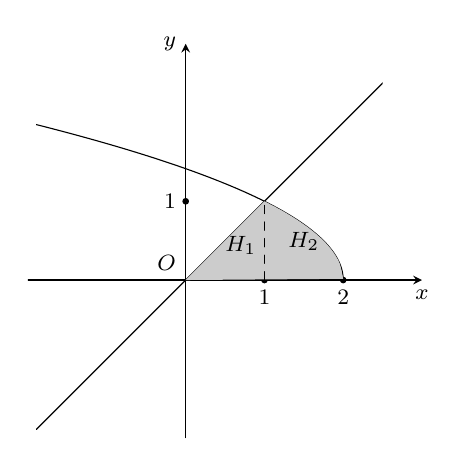
\begin{tikzpicture}[scale=1,>=stealth, font=\footnotesize, line join=round, line cap=round]
			
			\def\xmin{-2} \def\xmax{3}
			\def\ymin{-2} \def\ymax{3}		
			%		\draw[color=gray!50,dashed] (\xmin,\ymin) grid (\xmax,\ymax);
			\draw[->] (\xmin,0)--(\xmax,0) node [below]{$x$};
			\draw[->] (0,\ymin)--(0,\ymax) node [left]{$y$};
			\node at (0,0) [above left]{$O$};
			\clip (\xmin+0.1,\ymin+0.1) rectangle (\xmax-0.5,\ymax-0.1);
			\draw[smooth,samples=300] plot(\x,{\x});
			\begin{scope}
			\clip (\xmin+0.1,0) rectangle (\xmax-0.5,3);	
			\draw[smooth,samples=300] plot({2-(\x)^2},\x);
			\end{scope}
			
			\draw[fill=black](1,0)circle(1pt) (2,0)node[below]{$2$}circle(1pt) (0,1)node[left]{$1$}circle(1pt);
			\fill[gray!40,smooth]
			plot[domain=0:1] (\x,{(\x)})
			-- plot[domain=1:2] (\x,{sqrt(2-\x)})
			-- cycle;
			\draw[dashed](1,0)node[below]{$1$}--(1,1);
			\draw (0.7,0.2)node[above]{$H_1$} (1.5,0.25)node[above]{$H_2$};
			\end{tikzpicture}}}
\end{ex}
\begin{ex}%Câu 39.%[DuongPham - ĐCHT THPT]%[2D3B3-3]
	\immini{
		Quay hình phẳng $(H)$ như hình được tô đậm trong hình vẽ bên quanh trục $Ox$ ta được khối tròn xoay có thể tích là
		\choice
		{$V=\dfrac{46\pi }{9}$}
		{\True $V=\dfrac{46\pi }{15}$}
		{$V=\dfrac{23\pi }{9}$}
		{$V=13\pi $}}{\begin{tikzpicture}[line width=1.0pt,line join=round,>=stealth,x=1cm,y=1cm,scale=0.8]
		\draw[->] (-3,0)--(0,0) node[below right]{$O$}--(4,0) node[below]{$x$};
		\draw[->] (0,-1) --(0,3.5) node[right]{$y$};
		\foreach \x in {-2,-1,1,2}{
			\draw (\x,0) node[below]{$\x$} circle (1pt);
		}
		\clip(-2.8,-0.8) rectangle (3.5,3);
		\draw [domain=-1.5:1.5, samples=100] plot (\x, {1.732*(\x)^2});
		\draw [domain=-2:2, samples=100] plot (\x, {sqrt(4-(\x)^2)});
		\fill [pattern = north east lines, line width = 2pt,draw=none]%
		plot[domain=-1:1](\x, {1.732*(\x)^2}) plot[domain=-1:1](\x, {sqrt(4-(\x)^2)});
		\draw(1.1,2.2)node[right]{$y=\sqrt{3}x^2$};
		\end{tikzpicture}}
	\loigiai{
		Xét hệ phương trình: $\heva{&x^2+y^2=4\\&y=\sqrt{3}x^2}\Rightarrow x=-1\vee x=1$.\\
		Do $(H)$ đối xứng nhau qua $Oy$ nên.\\
		$V=2\pi\displaystyle\int\limits_0^{\sqrt{3}}\left[\left(4-x^2\right)-(\sqrt{3}x)^2\right]\mathrm{\,d}x-2\pi\displaystyle\int\limits_0^{\sqrt{3}}\left(4-x^2-3x^4\right)\mathrm{\,d}x=2\pi\left(4x-\dfrac{x^5}{3}-\dfrac{3x^5}{5}\right)\bigg|_0^{\sqrt{3}}=\dfrac{46\pi}{15}$.}
	%<MyLT>
\end{ex}
\begin{ex}%Câu 40.%[DuongPham - ĐCHT THPT]%[2D3K3-3]
	Thể tích $V$ của khối tròn xoay được sinh ra khi quay hình phẳng giới hạn bởi đường tròn $(C)\colon x^2+(y-3)^2=1$ xung quanh trục hoành là
	\choice
	{$V=6\pi$}
	{$V=6\pi^3$}
	{$V=3\pi^2$}
	{\True $V=6\pi^2$}
	\loigiai{
		\immini{	Ta có
			$x^2+(y-3)^2=1\Leftrightarrow y=3\pm\sqrt{1-x^2}$.\allowdisplaybreaks\begin{eqnarray*}
				V&=&\pi\displaystyle\int\limits_{-1}^1\left[\left(3+\sqrt{1-x^2}\right)^2-\left(3-\sqrt{1-x^2}\right)^2\right]\mathrm{\,d}x\\&=&12\pi\displaystyle\int\limits_{-1}^1\sqrt{1-x^2}\mathrm{\,d}x.		
			\end{eqnarray*}
			Đặt $x=\sin t\Rightarrow\mathrm{\,d}x=\cos t\cdot\mathrm{\,d}t$.\\
			Với $\heva{&x=1\Rightarrow t=\dfrac{\pi}{2}\\&x=-11\Rightarrow t=-\dfrac{\pi}{2}}$ \\
			$ \Rightarrow V=12\pi\displaystyle\int\limits_{-\tfrac{\pi}{2}}^{\tfrac{\pi}{2}}\sqrt{1-\sin^2t}\cdot\cos t\cdot\mathrm{\,d}t=12\pi\displaystyle\int\limits_{\tfrac{\pi}{2}}^{\tfrac{\pi}{2}}\cos^2 t\mathrm{\,d}t=6\pi^2 $.}{\begin{tikzpicture}[scale=0.8,>=stealth, font=\footnotesize, line join=round, line cap=round]
			
			\def\xmin{-2} \def\xmax{4}
			\def\ymin{-1} \def\ymax{5}
			
			
			\draw[->] (\xmin,0)--(\xmax,0) node [below]{$x$};
			\draw[->] (0,\ymin)--(0,\ymax) node [left]{$y$};
			\node at (0,0) [below left]{$O$};
			\clip (\xmin+0.1,\ymin+0.1) rectangle (\xmax-0.5,\ymax-0.1);
			\draw[thick,smooth,samples=300,domain=-1:1.001] plot(\x,{3+sqrt(1-(\x)^2)});
			\draw[pattern=north east lines](0,3)circle(1);
			\draw[dashed](-1,0)node[below]{$-1$}--(-1,3) (1,0)node[below]{$1$}--(1,3);
			\fill[black](0,3)node[right]{$3$}circle(1pt) (-1,0)circle(1pt) (1,0)circle(1pt) (1,3)circle(1pt) (-1,3)circle(1pt);
			\draw(0,4)node[above]{$f(x)=3+\sqrt{1-x^2}$} (0,2)node[below]{$g(x)=3-\sqrt{1-x^2}$};
			\end{tikzpicture}}}
\end{ex}
\begin{ex}%Câu 41.%[DuongPham - ĐCHT THPT]%[2D3B3-3]
	Trên mặt phẳng $Oxy$, cho hình phẳng $(H)$ giới hạn bởi các đường $(P)\colon y=x^2$; $(P')\colon ~y~=~4x^2$, $(d)\colon y=4$. Thể tích của khối tròn xoay khi quay $(H)$ quanh trục $Ox$ bằng 
	\choice
	{$\dfrac{9\pi}{5}$}
	{\True $\dfrac{4\pi}{5}$}
	{$\dfrac{7\pi}{5}$}
	{$2\pi$}
	\loigiai{
		\immini{Đặt $V$ là thể tích cần tìm.\\
			Xét phương trình hoành độ giao điểm của $(P)$ và $(d)$		$$x^2-4\Leftrightarrow\hoac{&x=2\\&x=-2.}$$
			Xét phương trình hoành độ giao điểm của $(P')$ và $(d)$:
			$$4x^2=4\Leftrightarrow\hoac{&x=1\\&x=-1.}$$ 
		}{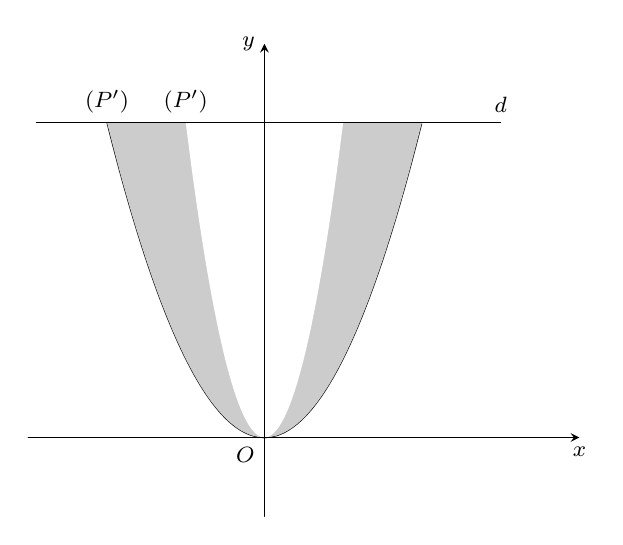
\begin{tikzpicture}[scale=1,>=stealth, font=\footnotesize, line join=round, line cap=round]
			\def\a{1} \def\b{0} \def\c{0} % Hệ số
			\def\e{4} \def\f{0} \def\g{0} % Hệ số
			\draw[smooth,samples=300,domain=-1:1] plot(\x,{\e*(\x)^2+\f*(\x)+\g});
			\begin{scope}
			\draw[smooth,samples=300,domain=-2:2] plot(\x,{\a*(\x)^2+\b*(\x)+\c});
			\fill[gray!40,smooth]
			plot[domain=-2:2] (\x,{\a*(\x)^2+\b*(\x)+\c})
			-- plot[domain=2:-2] (\x,{4})
			-- cycle;
			\fill[white!20,smooth]
			plot[domain=-1:1] (\x,{\e*(\x)^2+\f*(\x)+\g})
			-- plot[domain=1:-1] (\x,{4})
			-- cycle;
			\end{scope}
			\def\xmin{-3} \def\xmax{4}
			\def\ymin{-1} \def\ymax{5}
			
			
			
			\draw[->] (\xmin,0)--(\xmax,0) node [below]{$x$};
			\draw[->] (0,\ymin)--(0,\ymax) node [left]{$y$};
			\node at (0,0) [below left]{$O$};
			\clip (\xmin+0.1,\ymin+0.1) rectangle (\xmax-0.5,\ymax-0.1);
			\draw[smooth,samples=300,domain=-3:3] plot(\x,{4});		
			\draw(3,4)node[above]{$d$} (-1,4)node[above]{$(P')$} (-2,4)node[above]{$(P')$};
			\end{tikzpicture}}
		\noindent
		$V_{1}$ là thể tích khối tròn xoay sinh bởi khi quay $\hoac{&y=x^2\\&y=4\\&Oy}$ quanh $Ox$.\\
		$V_{2}$ là thể tích khối tròn xoay sinh bởi khi quay $\hoac{&y=4x^2\\&y=4\\&Oy}$ quanh $Ox$.\\ Lúc đó:
		\allowdisplaybreaks\begin{eqnarray*}
			V&=&V_1-V_2\\&=&\pi\displaystyle\int\limits_0^2\left[4-(x^2)^2\right]\mathrm{\,d}x-\pi\displaystyle\int\limits_0^2\left[4-\left(4x^2\right)^2\right]\mathrm{\,d}x\\&=&\pi\displaystyle\int\limits_0^2\left(4-x^2\right)\mathrm{\,d}x-\pi\displaystyle\int\limits_0^1\left(4-16x^4\right)\mathrm{\,d}x \\&=&\pi\left(4x-\dfrac{x^5}{5}\right)\bigg|_0^2-\pi\left(4x-16\dfrac{x^5}{5}\right)\bigg|_0^1=\pi\left(8-\dfrac{32}{5}-4+\dfrac{16}{5}\right)=\dfrac{4\pi}{5}\,\, \text{đvtt}.
		\end{eqnarray*}
	}
\end{ex}
\begin{ex}%Câu 42.%[DuongPham - ĐCHT THPT]%[2D3K3-3]
	\immini{	Bên trong hình vuông cạnh $a$, dựng hình sao cho bốn cạnh đều như hình vẽ bên (các kích thước cần thiết cho như ở trong hình). Tính thể tích của khối tròn xoay sinh ra khi quay hình sao đó quay trục $xy$. 
		\choice
		{\True $\dfrac{5\pi}{48}a^3$}
		{$\dfrac{5\pi}{16}a^3$}
		{$\dfrac{\pi}{6}a^3$}
		{$\dfrac{\pi}{8}a^3$}}{\begin{tikzpicture}[scale=0.8,>=stealth, font=\footnotesize, line join=round, line cap=round]
		\def\xmin{-2.5} \def\xmax{2.5}  \def\ymin{-2.5}  \def\ymax{3} 
		%	\draw[color=gray!50,dashed] (\xmin,\ymin) grid (\xmax,\ymax);
		%	\draw[->] (\xmin,0)--(\xmax,0) node [below]{$x$};
		\draw[->] (0,\ymin)node[left]{$y$}--(0,\ymax) node [left]{$x$};
		\clip (\xmin,\ymin) rectangle (\xmax,\ymax);
		%%%%
		\def\a{2}
		\path
		(\a,\a)coordinate(A)
		(-\a,\a)coordinate (B)
		;
		\draw[pattern=north east lines] (\a,\a)--(\a/2,0)--(\a,-\a)--(0,-\a/2)--(-\a,-\a)--(-\a/2,0)--(-\a,\a)--(0,\a/2)--cycle;
		\draw[<->, dashed](\a,\a)--(\a,0);\draw[<->, dashed] (\a,0)--(\a,-\a);\draw[<->, dashed] (\a,-\a)--(0,-\a);\draw[<->, dashed] (0,-\a)--(-\a,-\a);\draw[<->, dashed] (-\a,-\a)--(-\a,0);\draw[<->, dashed] (-\a,0)--(-\a,\a);\draw[<->, dashed] (-\a,\a)--(0,\a);\draw[<->, dashed] (0,\a)--(\a,\a);
		\draw[<->, dashed](\a/2,0)--(\a,0);
		\draw[<->, dashed](-\a,0)--(-\a/2,0);
		\draw[<->, dashed](0,\a)--(0,\a/2);
		\draw[<->, dashed](0,-\a)--(0,-\a/2); 
		\fill[black](\a,\a)circle(1pt) (-\a,\a)circle(1pt) (-\a,-\a)circle(1pt) (\a,-\a)circle(1pt);
		\draw(\a,\a/2)node[right]{$\tfrac{a}{2}$} (\a*0.75,0)node[above]{$\tfrac{a}{4}$};	
		\end{tikzpicture}}
	\loigiai{
		\immini{Gọi $V$ là thể tích khối tròn xoay cần tính.\\
			Gọi $V_1$ là thể tích khối tròn xoay khi quay hình phẳng được tô màu trong hình bên quanh trục hoành.\\
			Khi đó $V=2V_1$.\\
			Ta có $V_1=\pi\displaystyle\int\limits_0^{\tfrac{3}{2}}\left(\dfrac{x}{2}+\dfrac{a}{4}\right)^2\mathrm{\,d}x-\pi\displaystyle\int\limits_{\tfrac{3}{4}}^{\tfrac{3}{2}}\left(2x-\dfrac{a}{2}\right)^2\mathrm{\,d}x=\dfrac{5\pi}{96}a^3$.\\ 
			Suy ra $V=2V_1=\dfrac{5\pi}{48}a^3$.\\
		}{
			\begin{tikzpicture}[scale=0.8,>=stealth, font=\footnotesize, line join=round, line cap=round]
			\def\xmin{-1} \def\xmax{6}  \def\ymin{-1}  \def\ymax{3} 
			%	\draw[color=gray!50,dashed] (\xmin,\ymin) grid (\xmax,\ymax);
			\draw[->] (\xmin,0)--(\xmax,0) node [below]{$x$};
			\draw[->] (0,\ymin)--(0,\ymax) node [left]{$y$};
			\clip (\xmin,\ymin) rectangle (\xmax,\ymax);
			%%
			\node at (0,0) [below left]{$O$};
			\clip (\xmin+0.1,\ymin+0.1) rectangle (\xmax-0.5,\ymax-0.1);
			\draw[smooth,samples=300,domain=-0.5:4] plot(\x,{2*(\x)-2});
			\draw[smooth,samples=300,domain=-0.5:4] plot(\x,{0.5*(\x)+1});
			\draw[dashed](2,0)node[below]{$\tfrac{a}{2}$}|-(0,2)node[left]{$\tfrac{a}{2}$};
			\draw(0,2)circle(1pt) (2,0)circle(1pt) (1,0)node[below right]{$\tfrac{a}{4}$}circle(1pt) (0,1)node[above left]{$\tfrac{a}{4}$}circle(1pt) (2.5, 1.5)node[right,scale=0.7]{$y=\tfrac{x}{2}+\tfrac{a}{2}$} (2.1,2.3)node[left,scale=0.7]{$y=2x-\tfrac{a}{2}$};
			\fill[gray!40](1,0)--(2,2)--(0,1)--(0,0)--cycle;
			
			\end{tikzpicture}}
		\noindent
		\textbf{Cách 2:} Thể tích của hình nón có bán kính đáy bằng $\dfrac{a}{2}$ và chiều cao bằng $\dfrac{a}{4}$ là $V_2=\dfrac{1}{3}\pi\left(\dfrac{a}{2}\right)^2-\dfrac{a}{4}=\dfrac{\pi a^3}{48}$.\\
		Thể tích hình nón có bán kính đáy bằng $\dfrac{a}{2}$ và chiều cao bằng $a$ là $V_3=\dfrac{1}{3}\pi\left(\dfrac{a}{2}\right)^2a=\dfrac{\pi a^3}{12}$.\\
		Thể tích hình nón có bán kính đáy bằng $\dfrac{a}{4}$ và chiều cao bằng $\dfrac{a}{2}$ là $V_4=\dfrac{1}{3}\pi\left(\dfrac{a}{4}\right)^2\cdot\dfrac{a}{2}=\dfrac{\pi a^3}{96}$.\\
		Tính thể tích của khối tròn xoay sinh ra khi quay hình sao đó quanh trục $xy$ là\\
		$V_1=2\left[(V_3-V_4)-V_2\right]=2\left(\dfrac{\pi a^3}{12}-\dfrac{\pi a^3}{96}-\dfrac{\pi a^3}{48}\right)=\dfrac{5\pi a^3}{48}$.}
\end{ex}
\Closesolutionfile{ans}
% \DAPAN
\inputansbox{10}{ans/2D3-3.2}
\Opensolutionfile{ans}[ans/ansCD2D3-3.1-2]
\subsubsection{Các ví dụ}
\begin{dang}{Bài toán về chuyển động}
	\begin{itemize}
		\item Giả sử vật $ M $ chuyển động trên quãng đường có độ dài là $s$ trong khoảng thời gian $t$. Khi đó, vật $ M $ chuyển động với vận tốc trung bình là
		\[v=\dfrac{s}{t}.\]
		\item Tuy nhiên, chúng ta gặp rất nhiều trường hợp vật chuyển động không đều, vận tốc thay đổi liên tục tùy theo vị trí và thời gian. Ví dụ xe chạy trên đường gặp nhiều chướng ngại vật thì giảm tốc, chạy trên đường thông thoáng thì tăng tốc. Vì vậy ta cần phương pháp tính đúng vận tốc của xe tại mỗi thời điểm.
		\item Giả sử $v(t)$ là vận tốc của vật $M$ tại thời điểm $t$, và $s(t)$ là quãng đường vật đi được sau khoảng thời gian $t$ tính từ lúc bắt đầu chuyển động. Ta có mối liên hệ giữa $s(t)$ và $v(t)$. Đạo hàm của quãng đường là vận tốc.
		\[s'(t)=v(t).\]
		\item Nguyên hàm của vận tốc là quãng đường.
		\[s(t)= \int v(t)\mathrm{\,d}t.\]
		\item Từ đây ta cũng có quãng đường vật đi được trong khoảng thời gian $t\in[a;b]$ là
		\[\displaystyle\int\limits_a^b v(t)\mathrm{\,d}t=s(b)-s(a).\]
		\item Nếu gọi $a(t)$ là gia tốc của vật $M$ thì ta có mối liên hệ giữa $v(t)$ và $a(t)$.
		\item Đạo hàm của vận tốc chính là gia tốc.
		\[v'(t)=a(t).\]
		\item Nguyên hàm của gia tốc chính là vận tốc.
		\[v(t)= \int a(t)\mathrm{\,d}t.\]
	\end{itemize}
\end{dang}
\begin{vd}%[2D3Y3-7]%[Phạm Thế Sinh]%Ví dụ 1.
	Một ô tô đang chạy với vận tốc $10$ m/s thì tài xế đạp phanh;
	từ thời điểm đó, ô tô chuyển động chậm dần đều với vận tốc $ v(t)=-5t+10 $ (m/s), trong đó $ t $ là khoảng thời gian tính bằng giây, kể từ lúc đạp phanh. Hỏi từ lúc đạp phanh đến khi dừng hẳn, ô tô còn di chuyển được bao nhiêu mét?
	\choice
	{$0{,}2$ m}
	{$2$ m}
	{\True $10$ m}
	{$20$ m}
	\loigiai{
		\textbf{Phân tích bài toán}\\
		Ta có nguyên hàm của vận tốc $v(t)=-5t+10$ chính là quãng đường $s(t)$ mà ô tô đi được sau thời gian $ t $ giây kể từ lúc tài xế đạp phanh.\\
		Vào thời điểm ô tô bắt đầu đạp phanh ứng với $t=0$.\\
		Vào thời điểm ô tô dừng lại thì $v(t)=0\Leftrightarrow-5t+10=0\Leftrightarrow t=2$.\\
		Từ đây ta tính được quãng đường xe đi được từ lúc $t=0$ đến $t=2$ theo công thức $\displaystyle\int\limits_0^2 v(t)\mathrm{\,d}t$.\\
		Lúc bắt đầu đạp phanh, tức là tại thời điểm $ t_0 $, ô tô có vận tốc $v_0=10$ (m/s).\\
		Suy ra $v(t_0)=-5t_0+10=10\Leftrightarrow t_0=0$.\\
		Khi ô tô dừng lại tại thời điểm $t_1$ thì vận tốc $v_1=0$ (m/s). Suy ra $v(t_1)=-5t_1+10=0\Leftrightarrow t_1=2$.\\
		Ta có mối liên hệ giữa $ 2 $ đại lượng biến thiên quãng đường đi được $s(t)$ và vận tốc $v(t)$ là
		\textit{Nguyên hàm của vận tốc $v(t)$ chính là quãng đường đi được $s(t)$}. Suy ra quãng đường đi được từ lúc đạp phanh đến khi dừng lại là tích phân của hàm $v(t)$ khi thời gian $ t $ từ $ 0 $s đến $ 2 $s.
		\[\displaystyle\int\limits_0^2 v(t)\mathrm{\,d}t=\displaystyle\int\limits_0^2(-5t+10)\mathrm{\,d}t=\left(-5\dfrac{t^2}{2}+10t\right)\bigg|_0^2=10\; \mathrm{m}.\]
		\textbf{Bình luận:} Qua bài toán này ta cần lưu ý:\\
		Một là, nguyên hàm của vận tốc là quãng đường đi được của vật chuyển động.\\
		Hai là, nếu biết $ s(t) $ là nguyên hàm của $ v(t) $ thì quãng đường của vật đi được trong khoảng thời gian $t\in[a;b]$ được tính theo công thức $\displaystyle\int\limits_a^b v(t)\mathrm{\,d}t=s(b)-s(a)$.\\
		Ba là, bài toán có thể giải theo phong cách Vật lí. Từ lúc đạp phanh đến khi dừng hẳn, ô tô còn di chuyển quãng đường là $S=v_ot+\dfrac{1}{2}at^2$ trong đó $\heva{&a=-5\\&t=2\\&v_o=10}\Rightarrow S=10\cdot 2+\dfrac{1}{2}(-5)\cdot 2^2=10$ m.}
\end{vd}
\begin{vd}%[2D3K3-7]%[Phạm Thế Sinh]%Ví dụ 2.
	\immini{Một xe mô tô phân khối lớn sau khi chờ hết đèn đỏ đã bắt đầu phóng nhanh với vận tốc tăng liên tục được biểu thị bằng đồ thị là đường cong Parabol có hình bên. Biết rằng sau $ 15 $s thì xe đạt đến vận tốc cao nhất $60$ m/s và bắt đầu giảm tốc. Hỏi từ lúc bắt đầu đến lúc đạt vận tốc cao nhất thì xe đã đi được quãng đường bao nhiêu mét?}{
		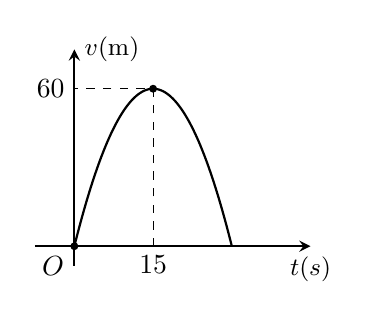
\begin{tikzpicture}[thick,>=stealth,scale=.5] 
		\draw[->] (-1,0) -- (6,0) node[below] {\small $t(s)$};
		\draw[->] (0,-.5) -- (0,5) node[right] {\small $v$(m)};
		\draw [fill=black] (0,0) node[below left]{$O$} circle (2pt) (2,4) circle (2pt);
		\draw [samples=100, domain= 0:4] plot (\x, {\x*(4-\x)});
		\draw[dashed,thin] (2,0) node[below]{$15$} |-(0,4) node[left]{$60$};
		\end{tikzpicture}
	}
	\loigiai{
		\begin{center}
			\begin{tikzpicture}[thick,>=stealth,join=round, cap=round,scale=.8] 
			\draw (0,0) -- (15,0) (0,.2) --++ (0,2);
			\draw[rounded corners=.5mm,fill=gray] (-.2,1.5) rectangle ++(.4,1);
			\draw[red,fill=red] (0,2.3) circle (3pt);
			\draw[yellow,fill=yellow] (0,2) circle (3pt);
			\shade [blue,shading=ball] (0,1.7) circle (3.5pt);
			\draw[fill=black] (0,0) circle (2pt) (15,0) circle (2pt);
			\draw[->] (0,-.7)node[scale=3,left,shift={(0,.1)}]{\faMotorcycle} --++ (2,0);
			\draw (8,0)node[below right]{$V_{max}=60$ m/s};
			\draw[fill=gray!30] (8.5,2.1)--++(0,-1)--++(-.25,0)--++(-60:1)--++(60:1)--++(-.25,0)--++(0,1) node[above]{$t=15$s}--cycle;
			\end{tikzpicture}
		\end{center}
		\textbf{Phân tích bài toán}\\
		Lúc ban đầu mô tô phóng nhanh với vận tốc thay đổi liên tục được biểu bằng đồ thị $(P)$ như hình vẽ, và đề bài chưa cho biểu thức vận tốc $v(t)$, cho nên ta cần tìm biểu thức vận tốc chuyển động.\\
		Vì đồ thị vận tốc có dạng là đường Parabol như hình vẽ nên biểu thức vận tốc sẽ có dạng $v(t)=at^2+bt+c$, đường cong Parabol có đỉnh $I(15;60)$, đồng thời đi qua gốc tọa độ $ O(0;0) $.\\
		Lúc bắt đầu tăng tốc xem như $t=0$, và theo đồ thị xe đạt vận tốc cao nhất vào thời điểm $t=15$.\\
		Nhắc lại rằng nguyên hàm của vận tốc $v(t)$ chính là quãng đường. Vậy quãng đường đi được của xe kể từ lúc tăng tốc ($t=0$ s) đến lúc đạt vận tốc cao nhất ($t=15$ s) tính theo công thức
		\[\displaystyle\int\limits_0^{15} v(t)\mathrm{\,d}t.\]
		Hàm vận tốc $ v(t)=at^2+bt+c $ có dạng là đường Parabol có đỉnh $I(15;60)$, đồng thời đi qua gốc tọa độ $O(0;0)$, suy ra
		\[\heva{&a{\cdot 0}^2+b\cdot 0+c=0\\&-\dfrac{b}{2a}=15\\&a{\cdot 15}^2+b\cdot 15+c=60}\Leftrightarrow\heva{&c=0\\&30a+b=0\\&a{\cdot 15}^2+b\cdot 15+0=60}\Leftrightarrow\heva{&c=0\\&a=-\dfrac{4}{15}\\&b=8} \Rightarrow v(t)=-\dfrac{4}{15}t^2+8t.\]
		%$ \Rightarrow v(t)=-\dfrac{4}{15}t^2+8t $.\\
		Theo đồ thị thì xe bắt đầu tăng tốc lúc $t=0$ và đạt vận tốc cao nhất lúc $t=15$s nên quãng đường đi được của xe từ lúc bắt đầu tăng tốc đến lúc đạt vận tốc cao nhất.
		\[\displaystyle\int\limits_0^{15} v(t)\mathrm{\,d}t=\displaystyle\int\limits_0^{15}\left(-\dfrac{4}{15}t^2+8t\right)\mathrm{\,d}t=\left(-\dfrac{4}{45}t^3+4t^2\right)\bigg|_0^{15}=600\; \mathrm{m}.\]
		Vậy từ lúc bắt đầu tăng tốc đến lúc đạt vận tốc cao nhất thì xe đã đi được một quãng đường dài $600$ m.\\
		\textbf{Bình luận:} Qua bài toán này ta cần lưu ý:\\
		Thông thường để tính tích phân $\displaystyle\int\limits_a^b f(x)\mathrm{\,d}x$ thì đề bài luôn cho sẵn biểu thức $f(x)$. Tuy nhiên, đối với ví dụ này, đề bài chỉ cho đồ thị của hàm $f(x)$ và học sinh phải thiết lập biểu thức $f(x)$. Đây là kĩ năng rất cần thiết vì trong quá trình học phổ thông, học sinh thường chỉ làm bài toán một chiều. Tức là, từ hàm số $f(x)$ vẽ thành đồ thị, rất ít khi (thậm chí là không có) học sinh gặp bài toán từ đồ thị suy ra biểu thức của hàm $f(x)$.}
\end{vd}
\begin{vd}%[2D3K3-7]%[Phạm Thế Sinh]%Ví dụ 3.
	\immini{Một máy bay đang chuyển động thẳng đều trên mặt đất với vận tốc $v=3$ (m/s) thì bắt đầu tăng tốc với độ biến thiên vận tốc là hàm số $a(t)$ có đồ thị hàm số là đường thẳng như hình bên. Sau $ 15 $s tăng tốc thì máy bay đạt đến vận tốc đủ lớn để phóng khỏi mặt đất. Hãy tính vận tốc khi máy bay bắt đầu rời khỏi mặt đất.}{
		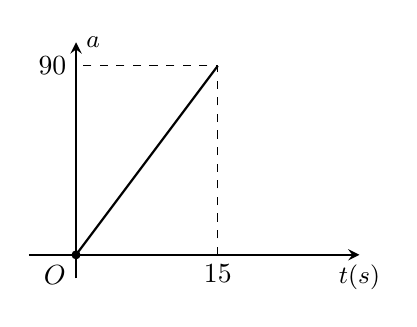
\begin{tikzpicture}[thick,>=stealth,scale=.6] 
		\draw[->] (-1,0) -- (6,0) node[below] {\small $t(s)$};
		\draw[->] (0,-.5) -- (0,4.5) node[right] {\small $a$};
		\draw [fill=black] (0,0) node[below left]{$O$} circle (2pt)--(3,4);
		\draw[dashed,thin] (3,0) node[below]{$15$} |-(0,4) node[left]{$90$};
		\end{tikzpicture}
	}
	\loigiai{
		\textbf{Phân tích bài toán}\\
		Máy bay bắt đầu tăng tốc với độ biến thiên vận tốc là hàm số $a(t)$, và đề bài chưa cho công thức $a(t)$, nên bước đầu ta cần tìm công thức $a(t)$.\\
		Vì đồ thị hàm số $a(t)$ là đường thẳng nên có dạng $a(t)=mt+n$, đường thẳng này đi qua gốc tọa độ $O(0;0)$ và điểm $ A(16;90) $ từ đó suy ra phương trình $a(t)$.\\
		\textit{Nhớ rằng}: Nguyên hàm của gia tốc $a(t)$ chính là vận tốc $v(t)$ của vật chuyển động nên ta có 
		\[v(t)=\int a(t)\mathrm{\,d}t.\]
		Chú ý điều kiện vận tốc của máy bay lúc bắt đầu tăng tốc là $v(0)=3$ (m/s), từ đây ta suy ra được hàm số $v(t)$.\\
		Để tính vận tốc của máy bay lúc rời khỏi mặt đất ta chỉ cần tính $v(15)$.\\
		Đường thẳng $a(t)=mt+n$ đi qua gốc tọa độ $O(0;0)$ và điểm $A(16;90)$ nên suy ra
		\[\heva{&m\cdot 0+n=0\\&m\cdot 15+n=90}\Leftrightarrow\heva{&n=0\\&m=6}\Rightarrow a(t)=6t.\]
		Ta hiểu rằng: Nguyên hàm của gia tốc $ a(t) $ chính là vận tốc của vật chuyển động. Do đó ta có công thức vận tốc $v(t)$ được tính theo công thức
		\[v(t)= \int a(t)\mathrm{\,d}t=\int 6t\mathrm{\,d}t=3t^2+C.\]
		Tại thời điểm bắt đầu tăng tốc thì xem như $ t=0 $ và vận tốc lúc đó là $ v=3 $ (m/s).\\
		Suy ra $ v(0)=0 \Leftrightarrow 3 \cdot 0^2+C=3 \Leftrightarrow C=3 \Rightarrow v(t)=3t^2+3 $.\\
		Vậy vận tốc máy bay đạt được khi bắt đầu phóng khỏi mặt đất là $ v(15)=3\cdot 15^2+3=678 $ (m/s).
		\textbf{Bình luận:} Qua bài toán này ta cần lưu ý:\\
		Một là, cho đồ thị của một hàm số, từ đó suy ra phương trình của hàm số đó.\\
		Hai là, nguyên hàm của gia tốc chính là vận tốc của vật chuyển động.}
\end{vd}
\begin{vd}%[2D3K3-7]%[Phạm Thế Sinh]%Ví dụ 4.
	Một viên đạn được bắn lên trời với vận tốc là $72$ m/s bắt đầu từ độ cao $2$ m. Hãy xác định chiều cao của viên đạn sau thời gian $5$s kể từ lúc bắn.
	\loigiai{
		\textbf{Phân tích bài toán}\\
		Để xác định được chiều cao của viên đạn tại thời điểm bất kì, ta cần tìm công thức quãng đường $ s(t) $ mà viên đạn đi được.\\
		Xem như tại thời điểm $ t_0=0 $ thì viên đạn được bắn lên. Theo giả thiết ta có $ s(0)=2 $ và $ v(0)=72 $.\\
		Ta biết rằng trong chuyển động ném đứng từ dưới lên thì gia tốc trọng trường có giá trị âm tại mọi thời điểm $ t $, nghĩa là $ a(t)=-9{,}8\;\mathrm{m/s^2} $.\\
		Vận tốc $ v(t) $ là nguyên hàm của $ a(t) $ nên ta có $ v(t)= \int -9{,}8\mathrm{\,d}t $, kết hợp điều kiện vận tốc ban đầu là $ v(0)=72 $ ta suy ra dạng của $ v(t) $.\\
		Tiếp tục có $ s(t) $ là nguyên hàm của $ v(t) $, kết hợp điều kiện vị trí ban đầu $ s(0)=2 $ ta tìm được phương trình của $ s(t) $. Từ đây ta tính được $ s(5) $.\\
		Ta có vận tốc của viên đạn tại thời điểm $ t $ là
		\[v(t)= \int -9{,}8\mathrm{\,d}t=-9{,}8t+C_1.\]
		Do $ v(0)=72 $ nên $ v(0)=-9{,}8\cdot 0+C_1=72 \Leftrightarrow C_1=72 \Rightarrow v(0)=-9{,}8t+72 $.\\
		Độ cao của viên đạn tại thời điểm $ t $ là
		\[s(t)=\int v(t)\mathrm{\,d}t=\int (-9{,}8t+72)\mathrm{\,d}t=-4{,}9t^2+72t+C_2.\]
		Vì $ s(0)=2 $ nên $ s(0)=-4{,}9 \cdot 0^2+72 \cdot 0+C_2=2 \Leftrightarrow C_2=2 \Rightarrow s(t)=-4{,}9t^2+72t+2 $.\\
		Vậy sau khoảng thời gian $5$s kể từ lúc bắn, viên đạn ở độ cao
		\[s(5)=-4{,}9 \cdot 5^2+72 \cdot 5+2=239{,}5\; \mathrm{m}.\]
		\textbf{Bình luận:} Qua bài toán này ta ta có bài toán tổng quát hơn cho chuyển động ném đứng từ dưới lên của vật. Giả sử vật $ A $ được ném thẳng đứng lên với vận tốc ban đầu $ v_0 $ ở vị trí độ cao $ s_0 $ so với mặt đất. Ta sẽ thiết lập các hàm vận tốc và hàm độ cao của vật $ A $ như sau:\\
		Xem như tại thời điểm $ t_0=0 $ thì vật được ném hướng lên. Theo giả thiết ta có $ s(0)=s_0 $ và $ s'(0)=v_0 $.\\
		Ta biết rằng trong chuyển động ném đứng từ dưới lên thì gia tốc trọng trường có giá trị âm tại mọi thời điểm $ t $, nghĩa là $ s'(t)=-9{,}8\;\mathrm{m/s^2} $.\\
		Ta có vận tốc của viên đạn tại thời điểm $ t $ là
		\[s'(t)= \int -9{,}8\mathrm{\,d}t=-9{,}8t+C_1.\]
		Do $ s'(t)=v_0 $ nên $ s'(t)=-9{,}8 \cdot 0+C_1 \Leftrightarrow C_1=v_0 \Rightarrow s'(t)=-9{,}8t+v_0 $.\\
		Độ cao của viên đạn tại thời điểm $ t $ là
		\[s(t)=\int s'(t)\mathrm{\,d}t=\int (-9{,}8t+v_0)\mathrm{\,d}t=-4{,}9t^2+v_0t+C_2.\]
		Vì $ s(0)=s_0 $ nên $ s(0)=-4{,}9 \cdot 0^2+72 \cdot 0+C_2=s_0 \Leftrightarrow C_2=s_0 \Rightarrow s(t)=-4{,}9t^2+v_0t+s_0 $.\\
		Vậy ta có hàm vận tốc $ s'(t)-9{,}8t+v_0 $ và hàm độ cao $ s(t)=-4{,}9t^2+v_0t+s_0 $.\\}
\end{vd}
\begin{dang}{Bài toán về công của lực tác dụng vào vật}
	\begin{itemize}
		\item Nếu một lực không đổi $ F $ tác dụng lên vật $ M $ dọc theo một khoảng cách (độ dời) $ d $, thì công $ W $ sinh ra trong quá trình dịch chuyển bằng tích của lực $ F $ và độ dài khoảng cách $ d $ mà nó đã tác dụng, ta có công thức
		\[W=F \cdot d.\]
		trong đó, lực $ F $ được hiểu là tác dụng dọc theo hướng (phương) chuyển động.
		\item Định nghĩa trên luôn đúng khi lực $ F $ không đổi. Tuy nhiên, nhiều trường hợp lực $ F $ biến thiên trong suốt quá trình thực hiện công. Trong các tình huống như vậy, người ta thường chia quá trình này thành nhiều phần nhỏ và tính công toàn phần nhờ lấy tổng các công tương ứng với các phần được chia (được tính nhờ phép tính tích phân).
		\immini{\item Giả sử $ f(x) $ là lực tác dụng lên vật tại vị trí $ x $, đường đi của lực tác dụng (quỹ đạo của vật được tác dụng lực) tương ứng với trục tọa độ $ Ox $. Khi đó, công toàn phần sinh ra trong cả quá trình chuyển động của vật từ vị trí $ x=a $ đến vị trí $ x=b $ là
			\[W= \displaystyle\int\limits_a^b f(x)\mathrm{\,d}x.\]}{
			\begin{tikzpicture}[thick,>=stealth,scale=.8] 
			\draw[->] (-1,0) -- (6,0) node[below] {\small $x$};
			\draw[->] (0,-1) -- (0,4.5) node[right] {\small $y$};
			\draw [fill=black] (1,2.4) circle (1pt) (4.5,2.6625) circle (1pt) (0,0) circle (1pt) node[below left] {\footnotesize $O$};
			\draw[smooth,domain=1:4.5,yscale=.15] plot(\x,{(\x-3)*(3-\x)+20});
			\fill [pattern=north west lines, opacity=0.5] plot[domain=1:4.5,yscale=.15] (\x,{(\x-3)*(3-\x)+20})|-(1,0);
			\draw[dashed,thin,yscale=.15] (1,0)node[below]{$a$}--(1,16) (4.5,0)node[below]{$b$}--(4.5,17.75);
			\draw (4,3)node[above]{$f(x)$} (2.7,1.2)node[above]{$W$};
			\end{tikzpicture}
		}
		
	\end{itemize}
\end{dang}

\begin{vd}%[2D3B3-7]%[Phạm Thế Sinh]%Ví dụ 1.
	\immini{Một lực $ 40 $N cần thiết để kéo căng một chiếc lò xo có độ dài tự nhiên từ $ 10 $ cm đến $ 15 $ cm. Hãy tính công sinh ra khi kéo lò xo từ độ dài từ $ 15 $ cm đến $ 18 $ cm.}{
		\begin{tikzpicture}[thick,>=stealth,line join=round,line cap=round,scale=.8] 
		\begin{scope}
		\draw[->] (0,2) |- (8,0) node[below] {\small $x$};
		\draw (0,1) -- (.2,1) (2.95,1) -- (3,1);
		\draw[decoration={aspect=0.3, segment length=1.5mm, amplitude=3mm,coil},decorate] (0.2,1) -- (2.95,1);
		\filldraw [pattern=north west lines, opacity=0.8] (3,0)|-(4,2)|-cycle;
		\draw (3.5,0)node[below]{$0$};
		\end{scope}
		
		\begin{scope}[shift={(0,-3.3)}]
		\draw[->] (0,2) |- (8,0) node[below] {\small $x$};
		\draw[->] (6,2.2) --++ (1.5,0) node[above,midway] {\small $f(x)=kx$};
		\draw (0,1) -- (.2,1);
		\draw[decoration={aspect=0.3, segment length=3mm, amplitude=3mm,coil},decorate] (0.2,1) -- (6,1);
		\filldraw [pattern=north west lines, opacity=0.8] (6,0)|-(7,2)|-cycle;
		\draw (3.5,0)node[below]{$0$} (6.5,-.4)node{$x$};
		\end{scope}
		\end{tikzpicture}
	}
	\loigiai{
		\textbf{Phân tích bài toán}\\
		Khi một lò xo bị biến dạng (bị nén hoặc kéo giãn) thì lò xo sẽ sinh ra một lực gọi là lực đàn hồi, lực đàn hồi này chống lại sự biến dạng, giúp lò xo trở về lại hình dạng tự nhiên ban đầu.\\
		Theo định luật Hooke: ``Khi một lò xo bị biến dạng (nén hoặc giãn) với một độ dài $ x;\ (x > 0) $ so với độ dài tự nhiên của lò xo thì lò xo sinh ra một lực đàn hồi có độ lớn bằng $ f(x)=kx$, trong đó $k$ là hệ số đàn hồi (hoặc độ cứng) của lò xo''.\\
		Dùng giả thiết để suy ra hàm số $ f(x)=kx $. Khi đó, công sinh ra khi kéo căng lò xo từ $ 15 $ cm đến $ 18 $ cm được tính theo công thức $ W= \displaystyle\int\limits_{0{,}15}^{0{,}18} f(x)\mathrm{\,d}x $.\\
		Ban đầu, lò xo có độ dài tự nhiên $ 10 $ cm. Dùng một lực $ 40 $N kéo giãn lò xo có độ dài $ 15 $ cm thì lò xo bị kéo dãn một đoạn có độ dài $ 5 $ cm = $ 0{,}05 $ m. Vậy ta có $ f(0{,}05)=40 $. Suy ra $ f(x)=800x $.\\
		Vậy công sinh ra khi kéo căng lò xo từ $ 15 $ cm đến $ 18 $ cm là
		\[W= \displaystyle\int\limits_{0{,}15}^{0{,}18} 800x\mathrm{\,d}x=800\cdot\dfrac{x^2}{2}\bigg|_{0{,}15}^{0{,}18}=1{,}56\;\mathrm{J}.\]}
\end{vd}
\begin{vd}%[2D3K3-7]%[Phạm Thế Sinh]%Ví dụ 2.
	\immini{Người thợ hồ nâng một xô nước bị rỉ lên cao $ 20 $ m với tốc độ cố định. Cho trọng lượng của xô là $ 3 $N, trọng lượng ban đầu của nước là $ 2 $N. Biết rằng xô nước bị rỉ nên lượng nước trong xô sẽ chảy ra với tốc độ không đổi trong thời gian nâng xô nước lên. Người ta ước tính rằng lượng nước trong xô sẽ thay đổi theo đồ thị là hình bên. Hỏi người thợ hồ đã dùng một công là bao nhiêu để nâng xô nước lên cao $ 20 $ m, với giả sử rằng bỏ qua trọng lượng sợi dây?}{
		\begin{tikzpicture}[line join=round,line cap=round,thick,xscale=.3,yscale=1.5] 
		\draw (-1,0) -- (20,0) node[right] {\small $x$};
		\foreach \x in{2,4,...,20} \draw (\x,0)--(\x,-2pt) node[below] {\scriptsize $\x$};
		\foreach \x in{0.4,0.8,...,20} \draw[thin] (\x,0)--(\x,-1pt);
		\foreach \y in{0.2,0.4,...,2} \draw (-7.5pt,\y)--(0,\y) node[left] {\scriptsize \pgfmathprintnumber[precision=2]{\y}};
		\draw (0,-.2) -- (0,2) node[shift={(1,.4)}] {\small Trọng lượng nước};
		\draw (0,0) node[below left]{\footnotesize $O$} (16,-.45) node{\footnotesize Độ cao của xô nước};
		\draw (20,0) -- (0,2);
		\end{tikzpicture}
	}
	\loigiai{
		\textbf{Phân tích bài toán}\\
		Trong suốt thời gian đưa xô nước lên độ cao $20$ m thì trọng lượng của xô không đổi, nhưng nước bị chảy ra liên tục nên trọng lượng nước thay đổi. Vì vậy để tính được công đưa xô nước lên cao thì ta tách làm hai loại công: Một là công đưa xô lên, hai là công đưa nước lên.\\
		Vì trọng lượng xô không đổi trong suốt thời gian đưa lên cao nên công cũng không đổi và tính bằng công thức
		\[W_{\text{xô}}=P_{\text{xô}}\cdot h=3\cdot 20=60\;\text{(Nm)}.\]\\
		Vì lượng nước giảm liên tục nên trọng lượng của nước là một hàm số $f(x)$ giảm liên tục phụ thuộc vào quãng đường $x$ mà xô đi được.\\
		Theo giả thiết đồ thị biểu diễn trọng lượng xô nước là đường thẳng có dạng $f(x)=ax+b$, dựa vào đồ thị ta tìm được phương trình $f(x)=ax+b$.\\
		Khi đó, công để đưa lượng nước lên cao $20$ m tính theo công thức
		\[\displaystyle\int\limits_0^{20} f(x)\mathrm{\,d}x.\]
		Vậy công cần thực hiện để đưa cả xô và nước lên cao $20$ m là
		\[60+\displaystyle\int\limits_0^{20} f(x)\mathrm{\,d}x.\] 
		Vì trọng lượng của xô là 3N không thay đổi nên công để đưa xô lên cao 20 m là
		\[ W_{\text{xô}}=P_{\text{xô}} \cdot h=3 \cdot 20=60.\] 
		Trọng lượng của nước thay đổi tùy thuộc vào độ cao của xô so với mặt đất. Gọi $x$ là độ cao của xô so với mặt đất, khi đó $ f(x)=ax+b$ là trọng lượng của nước tương ứng với độ cao $x$.\\
		Đồ thị hàm số $f(x)=ax+b$ đi qua hai điểm $A(0;2)$ và $B(20;0)$ nên
		\[\heva{&a \cdot 0+b=2\\&a \cdot 20+b=0}\Rightarrow \heva{&b=2\\&a=-\dfrac{1}{10}}\Rightarrow f(x)=-\dfrac{1}{10}x+2.\] 
		Công sinh ra khi đưa nước từ mặt đất lên cao $20$ là 
		\[\displaystyle\int\limits_0^{20} f(x)\mathrm{\,d}x=\displaystyle\int\limits_0^{20}\left(-\dfrac{1}{10}x+2\right) \mathrm{\,d}x=\left(-\dfrac{1}{10}x+2\right)\bigg|_{0}^{20}=20\;\text{(Nm)}.\]\\
		Vậy công toàn bộ để đưa cả xô và nước lên cao $20$ m là $60+20=80$ (Nm).\\
		Cho hàm số $f(x)$ biểu diễn cho sự tăng (hay giảm) số lượng của một đối tượng nào đó (số người, vi khuẩn, vi trùng, lượng nước chảy,...).\\
		Giá trị $f(x)$ là số lượng của đối tượng đó tại thời điểm $x$.\\
		Đạo hàm $f'(x)$ chính là tốc độ tăng (hay giảm) của đối tượng đó tại thời điểm $x$.\\
		Số lượng tăng thêm (hoặc giảm đi) của đối tượng trong khoảng $x\in \left[a;b\right]$ là
		\[\displaystyle\int\limits_a^b f(x)\mathrm{\,d}x.\]}
\end{vd}
\begin{dang}{Bài toán về tăng trưởng, phát triển}
\end{dang}
\begin{vd}%[2D3K3-7]%[Phạm Thế Sinh]%Ví dụ 1.
	Một nghiên cứu chỉ ra rằng sau $x$ tháng kể từ bây giờ, dân số của thành phố $A$ sẽ tăng với tốc độ $v(x)=10+2\sqrt{2x+1}$ (người/tháng). Dân số của thành phố sẽ tăng thêm bao nhiêu trong $4$ tháng tới.
	\loigiai{
		\textbf{Phân tích bài toán}\\
		Giả thiết cho $v(x)=10+2\sqrt{2x+1}$ hàm biểu thị cho tốc độ tăng dân số trong tháng thứ $x$. Vậy nguyên hàm của $v(x) $ chính là hàm số $f(x)$ biểu thị cho dân số của thành phố sau $x$ tháng kể từ bây giờ.\\
		Đề bài yêu cầu tính số dân tăng thêm của thành phố trong vòng 4 tháng tới. Theo lý thuyết đã nêu thì số dân tăng thêm đó được tính theo công thức. 
		\[\displaystyle\int\limits_0^4 v(t)\mathrm{\,d}t=f(4)-f(0).\] 
		Chú ý rằng ta có thể tính bằng $2$ cách. Cách $1$ là tìm nguyên hàm $f(x)$, sau đó tính hiệu số $f(4)-f(0)$. Cách $2$ là tính trực tiếp tích phân $\displaystyle\int\limits_0^4 v(t)\mathrm{\,d}t$.\\
		Gọi $f(x)$ là dân số của thành phố sau $x$ tháng kể từ bây giờ.\\
		Tốc độ thay đổi của dân số là $v(x)=10+2\sqrt{2x+1}$.\\ 
		Suy ra 
		\[f(x)=\displaystyle\int\limits \left(10+2\sqrt{2x+1}\right)\mathrm{\,d}x=10+2\displaystyle\int\limits 10+2\sqrt{2x+1}\mathrm{\,d}x.\]
		Mà $\displaystyle\int\limits \sqrt{2x+1}\mathrm{\,d}x=\dfrac{1}{2}\sqrt{2x+1}^{\frac{1}{2}}\mathrm{\,d}(2x+1)=\dfrac{1}{3}\left(2x+1\right)^{\frac{3}{2}}+C$.\\ 
		Do đó $f(x)=10x+\dfrac{2}{3}\left(2x+1\right)^{\frac{3}{2}}+C$.\\ 
		Số dân trong $4$ tháng tới là: 
		\[f(4)-f(0)=10\cdot 4+\dfrac{2}{3}\left(2x+1\right)^{\frac{3}{2}}+C-\left(0+\dfrac{2}{3}+C\right)\approx 57\;\text{người}.\]
		\textbf{Bình luận:} Qua bài toán này ta cần lưu ý:\\
		Một là, nếu gọi $f(x)$ là số dân thay đổi theo thời gian x thì đạo hàm $f’(x)$ chính là tốc độ thay đổi (tăng hoặc giảm) của số dân.\\
		Hai là, nguyên hàm của hàm tốc độ tăng giảm $f’(x)$ chính là hàm $f(x)$ biểu thị cho dân số.\\
		Ba là, bài toán có thể giải theo cách thứ $2$. Vì $v(x)$ là tốc độ tăng dân số từ bây giờ $(x = 0)$ đến tháng thứ $4$ $(t = 4)$ nên số dân tăng thêm (hoặc giảm đi) trong thời gian đó là
		\[\displaystyle\int\limits_0^4 v(x)\mathrm{\,d}x=\displaystyle\int\limits \left(10+2\sqrt{2x+1}\right)\mathrm{\,d}x= \left(10+\dfrac{4}{3}\left(2x+1\right)^{\frac{3}{2}}\right)\bigg|_{0}^{4}\approx 57\;\text{người}.\]
		\[\displaystyle\int\limits_a^b f'(t)\mathrm{\,d}t=f(b)-f(a).\]}
\end{vd}
\begin{vd}%[2D3B3-7]%[Phạm Thế Sinh]%Ví dụ 2.
	Tốc độ thay đổi của số lượng người $V$ (tính bằng ngàn người) tham gia công tác tình nguyện ở nước Mỹ từ năm $2000$ đến năm $2006$ có thể được mô hình bởi hàm số $v(t)=119{,}85t^2-30e^t+37{,}26e^{-t}$ với $t$ là năm ($t = 0$ ứng với năm $2000$).\\
	Hỏi số lượng người tham gia tình nguyện trong giai đoạn trên tăng lên hay giảm đi với số lượng bao nhiêu. (Nguồn: Cục thống kê lao động nước Mỹ)
	\loigiai{
		\textbf{Phân tích bài toán}\\
		Hàm số $v(t)=119{,}85t^2-30e^t+37{,}26e^{-t}$ biểu thị cho tốc độ thay đổi số lượng người tham gia công tác tại năm thứ $ t $ (tính từ năm $2000$ đến năm $2006$).\\
		Suy ra nguyên hàm $ S(t) $ của $ v(t) $ chính là số lượng người tham gia công tác tại năm thứ $t$.\\
		Đề bài yêu cầu tính số lượng người thay đổi (tăng lên hay giảm đi) trong khoảng từ năm $2000$ đến năm $2006$. Số lượng này chính được tính bằng công thức
		\[\displaystyle\int\limits_0^6 v(t)\mathrm{\,d}t=S(6)-S(0).\]
		trong đó $ t=0 $ ứng với năm $2000$, $ t=6 $ ứng với năm $2006$.\\
		Sự chênh lệch của số người tham gia tình nguyện trong giai đoạn từ năm $2000$ đến năm $2006$ là
		\begin{eqnarray*}
			\displaystyle\int\limits_0^6 v(t)\mathrm{\,d}t&=&\displaystyle\int\limits_0^6 \left(119{,}85t^2-30e^t+37,26e^{-t}\right)\mathrm{\,d}t\\
			&=&\left(\dfrac{119{,}85}{3}t^3-30e^t-37{,}26e^{-t}\right)\bigg|_{0}^{6}=-3473{,}756166-(-67,26)\approx -3406. 
		\end{eqnarray*}
		Vậy trong khoảng thời gian từ năm $2000$ đến năm $2006$, số lượng người tham gia công tác tình nguyện đã giảm đi khoảng $3406$ người.}
\end{vd}
\begin{vd}%[2D3B3-7]%[Phạm Thế Sinh]%Ví dụ 3.
	Tốc độ tăng các cặp đôi kết hôn (đơn vị tính: triệu người) của nước Mỹ từ năm $1970$ đến năm $2005$ có thể được mô hình bởi hàm số $f(t)=1{,}218t^2-44{,}72t+709{,}1$ với $t$ là năm ($t = 0$ ứng với năm $1970$). Số lượng cặp đôi kết hôn vào năm $2005$ là $59\,513$ ngàn người.
	\begin{listEX}[1]
		\item Tìm một mô hình biểu thị cho số lượng các cặp đôi kết hôn của nước Mỹ.
		\item Sử dụng mô hình đó để dự đoán số lượng các cặp đôi kết hôn của nước Mỹ vào năm $2012$. Kết quả của bạn liệu có hợp lí? Giải thích vì sao?
	\end{listEX}
	\loigiai{
		\textbf{Phân tích bài toán}\\
		Ở đây ta hiểu rằng năm $1970$ ứng với $t=0 $ và năm $2005$ ứng với $t=35$.\\
		Hàm số $f(t)=1{,}218t^2-44{,}72t+709{,}1$ biểu thị cho tốc độ tăng các cặp đôi kết hôn vào năm thứ $t$.\\
		Suy ra nguyên hàm của $f(t)$ là hàm số $ F(t) $ biểu thị cho số lượng cặp đôi kết hôn vào năm thứ $t$.\\
		Dựa vào điều này ta tìm ra mô hình $ F(t) $ với điều kiện $ F(35)=59\,513$.\\ 
		Từ mô hình $ F(t) $ ta có thể tính được số lượng cặp đôi kết hôn vào năm bất kì trong khoảng từ năm $1970$ đến $2005$.
		\begin{listEX}[1]
			\item Để tìm một mô hình cho số lượng các cặp đôi kết hôn ta tìm nguyên hàm của $ f(t) $
			\begin{eqnarray*}
				F(t)&=&\displaystyle\int\limits \left(1{,}218t^2-44{,}72t+709{,}1\right)\mathrm{\,d}t=\dfrac{1{,}218}{3}t^3-\dfrac{44{,}72}{2}t^2+709{,}1t+C\\
				&=&0{,}406t^3-22{,}36t^2+709{,}1t+C. 
			\end{eqnarray*}
			Số lượng các cặp đôi kết hôn vào năm $2005$ là $59513$ triệu người nên ta có
			\[F(35)=59\,513 \Leftrightarrow 0{,}406 \cdot 35^3-22{,}36\cdot 35^2+709{,}1 \cdot 35+C=59\,513\Leftrightarrow C=44\,678{,}25.\]
			Vậy một mô hình cần tìm là $F(t)=0{,}406t^3-22{,}36t^2+709{,}1t+44\,678{,}25$.
			\item Số lượng các cặp đôi kết hôn vào năm $2012$ là $ F(42)=65\,097{,}138$ triệu người.\\
			Theo báo cáo của Cục điều tra dân số nước Mỹ thì vào năm $2012$ tổng số các cặp đôi kết hôn của nước Mỹ khoảng $61{,}047$ triệu người. So với kết quả lý thuyết thì sự chênh lệch là tạm chấp nhận được.
		\end{listEX}
	}
\end{vd}
\begin{vd}%[2D3K3-7]%[Phạm Thế Sinh]%Ví dụ 4.
	Tốc độ phát triển của số lượng vi khuẩn trong hồ bơi được mô hình bởi hàm số $ B'(t)=\dfrac{1000}{(1+0{,}3t)^2},\ t\geq 0 $, trong đó $B(t)$ là số lượng vi khuẩn trên mỗi ml nước tại ngày thứ $t$. Số lượng vi khuẩn ban đầu là $500$ con trên mỗi ml nước. Biết rằng mức độ an toàn cho người sử dụng hồ bơi là số vi khuẩn phải dưới $3000$ con trên mỗi ml nước. Hỏi sau bao nhiêu ngày thì người ta phải xử lí và thay nước mới cho hồ bơi.
	\loigiai{
		\textbf{Phân tích bài toán}\\
		Để biết được sau bao nhiêu ngày phải thay nước mới cho hồ bơi thì ta cần xác định sau bao nghiêu ngày thì số lượng vi khuẩn phát triển đến $3000$ con trên mỗi ml nước. Như vậy ta phải xác định hàm số $B(t)$ biểu thị cho số lượng phát triển của vi khuẩn tại ngày thứ $t$.\\
		Ta biết rằng tốc độ phát triển của số lượng vi khuẩn trong hồ bơi được mô hình bởi hàm số $B'(t)=\dfrac{1000}{(1+0{,}3t)^2}$. Suy ra nguyên hàm của $ B'(t) $ là hàm số $B(t)$ biểu thị cho số lượng của vi khuẩn tại ngày thứ $t$.\\
		Khi đó, kết hợp với điều kiện số lượng vi khuẩn lúc đầu $B(0) = 500$ con, ta tìm được một mô hình $B(t)$ biểu thị cho số lượng vi khuẩn tại ngày thứ $t$.\\
		Từ đây ta có thể tính số lượng vi khuẩn tại thời điểm tùy ý và xác định được người bơi có an toàn hay không? Có nên thay nước cho hồ bơi hay không?\\
		Số lượng của vi khuẩn tại ngày thứ $t$ được mô hình bởi hàm số $B(t)$ là nguyên hàm của $B’(t)$. 
		\[B’(t)=\displaystyle\int \dfrac{1000}{(1+0{,}3t)^2}\mathrm{\,d}t=1000\displaystyle\int (1+0{,}3t)^{-2}\mathrm{\,d}t=-\dfrac{1000}{0{,}3(1+0{,}3t)}+C.\]
		Số lượng vi khuẩn lúc ban đầu là $500$ con trên mỗi ml nước nên
		\[B(0)=500\Leftrightarrow -\dfrac{1000}{0{,}3(1+0{,}3.0)}+C=500\Leftrightarrow C=\dfrac{11\,500}{3}.\]		
		Suy ra hàm số biểu thị cho số lượng vi khuẩn tại ngày thứ t là
		\[B(t)= -\dfrac{1000}{0{,}3(1+0{,}3t)}+\dfrac{11\,500}{3}.\] 
		Số lượng vi khuẩn dưới $3000$ con trên mỗi ml nước thì người bơi vẫn an toàn; và người bơi không an toàn khi
		\[B(t)\geq 3000\Leftrightarrow -\dfrac{1000}{0{,}3(1+0{,}3t)}+\dfrac{11\,500}{3}\geq 3000 \Leftrightarrow \dfrac{1000}{0{,}3(1+0{,}3t)}\geq \dfrac{2500}{3}\Leftrightarrow 1+0{,}3t\geq 4\Leftrightarrow t\geq 10.\]
		Vậy vào ngày thứ $10$ thì số lượng vi khuẩn sẽ là $3000$ con và hồ bơi không còn an toàn, cần phải thay nước mới.}
\end{vd}
\begin{vd}%[2D3B3-7]%[Phạm Thế Sinh]%Ví dụ 5.
	Một hồ nước bị ô nhiễm được xử lý bằng một chất diệt khuẩn. Tốc độ phát triển của số lượng vi khuẩn sống sót được mô hình bởi $B'(t)=\dfrac{3000}{(1+0{,}2t)^2},\ t \geq 0$ với $B(t)$ là số lượng vi khuẩn trên mỗi ml nước là $t$ là số ngày tính từ khi hồ nước được xử lý. Biết số lượng vi khuẩn ban đầu là $10\,000$ con/ml nước. Sử dụng mô hình này xác định số lượng vi khuẩn sau $5$ ngày. Liệu số lượng vi khuẩn có thể vượt $2000$ con/ml nước.
	\loigiai{
		\textbf{Phân tích bài toán}\\
		Theo giả thiết, tốc độ phát triển của số lượng vi khuẩn sống sót được mô hình bởi công thức $B'(t)=\dfrac{3000}{(1+0{,}2t)^2},\ t \geq 0$ với $t$ là số ngày tính từ khi hồ bơi được xử lí. Suy ra nguyên hàm của $ B'(t) $ là hàm số $ B(t) $ biểu thị cho số lượng vi khuẩn trên mỗi ml nước tại ngày thứ $t$ (kể từ lúc hồ nước được xử lí).\\
		Kết hợp với điều kiện số lượng vi khuẩn ban đầu là $B(0) = 10\,000$ con/ml nước, ta tìm được mô hình $ B(t)$. Từ đây ta tính được $ B(5)$ là số lượng vi khuẩn sống sót sau $5$ ngày kể từ khi hồ nước được xử lí.\\
		Tốc độ phát triển của số lượng vi khuẩn sống sót được mô hình bởi công thức đạo hàm $B'(t)=\dfrac{3000}{(1+0{,}2t)^2},\ t \geq 0$ 
		Nguyên hàm của $B'(t)$ là hàm $B(t)$ biểu thị số lượng vi khuẩn sống sót trong ngày thứ $t$. Ta có
		\[B(t)=\int \dfrac{-3000}{(1+0{,}2t)^2}\mathrm{\,d}t=-3000\int (1+0{,}2t)^{-2}\mathrm{\,d}t=15\,000(1+0{,}2t)^{-1}+C=\dfrac{15\,000}{1+0{,}2t}+C.\]
		Vì số lượng vi khuẩn ban đầu là $10\,000$ con/ml nước nên có
		\[B(0)=10\,000\Rightarrow 15\,000+C=10\,000\Rightarrow C=-5000.\]
		Vậy hàm số biểu thị số lượng vi khuẩn sống sót tại ngày thứ $t$ là
		\[B(t)=\dfrac{15\,000}{1+0{,}2t}-5000.\]
		Số vi khuẩn sau $5$ ngày sẽ là $B(2)=2500$ con/$1$ ml.\\ 
		Như vậy số lượng vi khuẩn đã vượt qua $2000$ con/ml nước.}
\end{vd}
\begin{vd}%[2D3K3-7]%[Phạm Thế Sinh]%Ví dụ 6.
	Người ta thay nước mới cho một bể bơi có dạng hình hộp chữ nhật có độ sâu là $h_1=280$ cm. Giả sử $h(t)$ là chiều cao (tính bằng cm) của mực nước bơm được tại thời điểm $t$ giây, biết rằng tốc độ tăng của chiều cao mực nước tại giây thứ $t$ là $ h'(t)=\dfrac{1}{500}\sqrt[3]{t+3} $ và lúc đầu hồ bơi không có nước. Hỏi sau bao lâu thì nước bơm được $ \dfrac{3}{4} $ độ sâu của hồ bơi?
	\loigiai{
		\textbf{Phân tích bài toán}\\
		Tốc độ tăng của chiều cao mực nước tại giây thứ $t$ là $ h'(t)=\dfrac{1}{500}\sqrt[3]{t+3} $. Suy ra nguyên hàm của $h’(t)$ chính là chiều cao của mực nước đã bơm được tại thời điểm $t$. Ta sẽ tính công thức nguyên hàm $h(t)$.\\
		Kết hợp với điều kiện lúc ban đầu hồ không chứa nước, tức là độ cao của mực nước trong hồ tại thời điểm $t = 0$ là $h(0) = 0$. Ta suy ra mô hình hàm số $h(t)$ biểu thị cho chiều cao của mực nước bơm được tại thời điểm $t$.\\
		Từ đây ta có thể xác định được thời gian để bơm được lượng nước bằng $\dfrac{3}{4} $ độ sâu của hồ bơi.\\
		Ta biết rằng chiều cao $h(t)$ của mực nước bơm được chính là nguyên hàm của tốc độ tăng $h’(t)$ của chiều cao mực nước.
		\[h(t)=\int h'(t)\mathrm{\,d}t=\int \dfrac{1}{500}\sqrt[3]{t+3}\mathrm{\,d}t=\dfrac{3}{2000}(t+3)^{\frac{4}{3}}+C.\]
		Lúc ban đầu (tại $ t=0 $) hồ bơi không chứa nước, nghĩa là
		\[h(t)=0\Leftrightarrow \dfrac{3}{2000}(t+3)^{\frac{4}{3}}+C=0\Leftrightarrow C=-\dfrac{3^{\frac{4}{3}}}{2000}.\]
		Suy ra mực nước bơm được tại thời điểm $t$ giây là
		\[h(t)= \dfrac{3}{2000}(t+3)^{\frac{4}{3}}-\dfrac{3^{\frac{4}{3}}}{2000}.\]
		Theo giả thiết, lượng nước bơm được bằng $\dfrac{3}{4}$ độ sâu của hồ bơi nên ta có
		\[h(t)=\dfrac{3}{4}h_1\Leftrightarrow  \dfrac{3}{2000}(t+3)^{\frac{4}{3}}-\dfrac{3^{\frac{4}{3}}}{2000}=\dfrac{3}{4} \cdot 280\Leftrightarrow 3^{\frac{4}{3}}=140\,004{,}33\Leftrightarrow t=7234\text{s}.\]
		Vậy sau khoảng thời gian $2$ giờ $34$ giây thì bơm được $\dfrac{3}{4}$ độ sâu của hồ bơi.}
\end{vd}
\begin{vd}%[2D3B3-7]%[Phạm Thế Sinh]%Ví dụ 7.
	Trong một đợt xả lũ, nhà máy thủy điện Hố Hô đã xả lũ trong $40$ phút với tốc độ lưu lượng nước tại thời điểm $t$ giây là $v(t)=10t+500$ (m$^3$/s). Hỏi sau thời gian xả lũ trên thì hồ chứa nước của nhà máy đã thoát đi một lượng nước là bao nhiêu?
	\loigiai{
		\textbf{Phân tích bài toán}\\
		Trong $40$ phút, nhà máy thủy điện xả lũ với tốc độ $v(t)=10t+500$ (m$^3$/s). Nguyên hàm của $ v'(t) $ chính là hàm số $f(t)$ biểu thị cho lượng nước đã xả tại thời điểm $t$.\\
		Lượng nước xả được trong thời gian $40$ phút (ứng với $2400$ giây) bằng tích phân $\displaystyle\int\limits_0^{2400} v'(t)\mathrm{\,d}t$.\\
		Như vậy, bằng phép tính này ta đã xác định được lượng nước đã thoát ra.\\
		Lượng nước lũ đã xả trong khoảng thời gian $40$ phút ($2400$ giây) sẽ bằng
		\[L=\displaystyle\int\limits_0^{2400} v'(t)\mathrm{\,d}t=\displaystyle\int\limits_0^{2400} (10t+500)\mathrm{\,d}t=(5t^2+500t)\bigg|_0^{2400}=3.10^7 \mathrm{m^3}.\]
		Vậy trong khoảng thời gian $40$ phút, nhà máy đã xả một lượng nước là $30$ triệu khối, tức là hồ chứa nước đã thoát đi $30$ triệu khối nước.}
\end{vd}
\begin{vd}%[2D3G3-7]%[Phạm Thế Sinh]%Ví dụ 8.
	Trọng lượng của một bào thai người nặng khoảng $0{,}04$ ounce. ($1$ ounce $= 28{,}3495$ gram) sau $8$ tuần tuổi. Trong suốt $35$ tuần tiếp theo, trọng lượng của bào thai này được dự đoán tăng với tốc độ: $B'(t)=\dfrac{2436e^{-0{,}193t}}{(1+784e^{-0{,}193t})^2},\ 8\leq t \leq 43$ với $B(t)$ là cân nặng tính bằng ounce và $t$ là thời gian tính bằng tuần. Hãy tính trọng lượng của bào thai sau $25$ tuần tuổi.
	\loigiai{
		\textbf{Phân tích bài toán}\\
		Tốc độ tăng của trọng lượng bào thai được mô hình bởi hàm số
		\[B'(t)=\dfrac{2436e^{-0{,}193t}}{(1+784e^{-0{,}193t})^2},\ 8\leq t \leq 43.\]
		Nguyên hàm của $B'(t) $ chính là hàm số $B(t) $ biểu thị cho cân nặng của bào thai tại thời điểm $t$ (tính bằng tuần).\\
		Kết hợp với điều kiện trọng lượng ban đầu của bào thai $ B(8)=0{,}04$, ta sẽ tìm ra hàm số $B(t)$. Từ đây ta có thể dự đoán được trọng lượng của bào thai trong thời gian sắp tới.\\
		Theo giả thiết thì trọng lượng của bào thai này được dự đoán tăng với tốc độ là hàm số
		\[B'(t)=\dfrac{2436e^{-0{,}193t}}{(1+784e^{-0{,}193t})^2},\ 8\leq t \leq 43.\] nên $B(t)$ chính là nguyên hàm của $B’(t)$.
		\[B(t)=\int \dfrac{2436e^{-0{,}193t}}{(1+784e^{-0{,}193t})^2}\mathrm{\,d}t.\]
		Đặt $ u=1+784e^{-0{,}193t}$, ta có
		\begin{eqnarray*}
			&& B(t)\approx -16,1\int \dfrac{\mathrm{\,d}u}{u^2}=\dfrac{16{,}1}{u}+C=\dfrac{16{,}1}{1+784e^{-0{,}193t}}+C\\
			&\Rightarrow &B(t)\approx \dfrac{16,1}{1+784e^{-0{,}193t}}+C. 
		\end{eqnarray*}
		Sau $8$ tuần tuổi thì bào thai cân nặng khoảng $0{,}04$ ounce nên
		\[B(8)=0{,}04\Rightarrow \dfrac{16{,}1}{1+784e^{-0{,}193.8}}+C=0{,}04\Rightarrow C=-0{,}0556.\]
		Do đó ta có hàm số cân nặng của bào thai là
		\[B(t)\approx \dfrac{16{,}1}{1+784e^{-0{,}193t}}-0{,}0556,\ 8\leq t \leq 43.\]
		Cân nặng của bào thai sau $25$ tuần tuổi là
		\[B(25)\approx \dfrac{16{,}1}{1+784e^{-0{,}193.25}}-0{,}0556=2{,}152\;\text{ounce}.\] 
	}
\end{vd}
\begin{dang}{Bài toán về kinh tế}
\end{dang}
\begin{vd}%[2D3Y3-7]%[Phạm Thế Sinh]%Ví dụ 1.
	Sau $t$ giờ làm việc một người công nhân có thể sản xuất với tốc độ là $q(t)=100+e^{-0{,}5t}$ đơn vị sản phẩm trong $1$ giờ. Giả sử người đó bắt đầu làm việc từ lúc $8$ giờ sáng. Hỏi người đó sẽ sản xuất được bao nhiêu đơn vị sản phẩm giữa $9$ giờ sáng và $11$ giờ trưa?
	\loigiai{
		\textbf{Phân tích bài toán}\\
		Đề bài cho hàm $q(t)=100+e^{-0{,}5t}$ mô tả tốc độ sản xuất sản phẩm của một người công nhân. Suy ra nguyên hàm của $ q(t) $ là hàm số $ S(t) $ mô tả số lượng sản phẩm làm ra của người công nhân đó trong $t$ giờ.\\
		Lúc $8$ giờ người công nhân đó bắt đầu làm việc (ta xem như $t = 0$). Như vậy thời gian từ $9$ giờ sáng đến $11$ giờ ứng với $t$ từ $1$ đến $4$.
		Số đơn vị sản phẩm người công nhân đó làm được từ $9$ giờ đến $11$ giờ là
		\[\displaystyle\int\limits_1^4 q(t)\mathrm{\,d}t.\]
		Gọi $ S(t) $ là số đơn vị sản phẩm mà công nhân sản xuất được sau $t$ giờ tính từ lúc $8$ giờ sáng.\\
		Ta có: $ S'(t)= q(t)=100+e^{-0{,}5t}$. \\
		Số đơn vị sản phẩm người đó sản xuất được từ $9$ giờ sáng $ t=1$ đến $11$ giờ trưa $ t=4 $ là
		\[\displaystyle\int\limits_1^4 q(t)\mathrm{\,d}t=\displaystyle\int\limits_1^4 (100+e^{-0{,}5t})\mathrm{\,d}t=(100t+2e^{-0{,}5t})\bigg|_1^4=200{,}76\ \text{đơn vị sản phẩm}.\]}
\end{vd}
\begin{vd}%[2D3K3-7]%[Phạm Thế Sinh]%Ví dụ 2.
	Qua điều tra các nhà phân tích kinh tế đã nhận định rằng tốc độ tăng trưởng kinh tế (GDP) của một quốc gia sau $t$ năm tính từ đầu năm $2004$ là $ 30+\dfrac{1}{2}\sqrt{5+t} $ tỷ USD/năm. Biết rằng GDP của quốc gia đó vào đầu năm $2004$ là $100$ tỷ USD. Hãy dự đoán GDP của quốc gia đó vào đầu năm $2015$.
	\loigiai{
		\textbf{Phân tích bài toán}\\
		Tốc độ tăng trưởng kinh tế (GDP) của quốc gia đó sau $t$ năm tính từ năm $2004$ được mô tả bởi hàm số $ q(t)= 30+\dfrac{1}{2}\sqrt{5+t}$. Suy ra nguyên hàm của $ q(t) $ là hàm số $ S(t) $ biểu thị GDP của quốc gia đó sau $t$ năm.\\
		Ta có: $ S(t)=\int q(t) \mathrm{\,d}t$.\\ 
		Năm $2004$ xem như $t = 0$, năm $2015$ ứng với $t = 11$. Giá trị tăng thêm GDP của quốc gia đó từ năm $2004$ đến $2015$ được tính theo công thức
		\[\displaystyle\int\limits_0^{11} q(t)\mathrm{\,d}t=S(11)-S(0).\]
		Vậy tổng giá trị GDP của quốc gia đó tính đến năm $2015$ bằng giá trị GDP năm $2004$ cộng thêm GDP từ năm $2004$ đến đầu năm $2015$, tính theo công thức
		\[\displaystyle\int\limits_0^{11} q(t)\mathrm{\,d}t+100.\]
		Nguyên hàm của $ q(t)= 30+\dfrac{1}{2}\sqrt{5+t} $ là hàm số $ S(t) $ mô tả GDP của quốc gia sau $t$ năm (được tính từ năm $2004$).\\
		GDP tăng thêm tính từ năm $2004\ (t = 0)$ đến đầu năm $2015\ (t = 11)$ là
		\[\displaystyle\int\limits_0^{11} q(t)\mathrm{\,d}t=\displaystyle\int\limits_0^{11} (30+\dfrac{1}{2}\sqrt{5+t})\mathrm{\,d}t=(30+\dfrac{1}{2}\sqrt{5+t})\bigg|_0^{11}=347,6\ \text{tỷ USD}.\] 
		Như vậy, tổng giá trị GDP tính đến đầu năm $2015$ bằng
		\[347,6+100=447,6\ \text{tỷ USD}.\]
		\textbf{Bình luận:} Qua bài toán này ta cần lưu ý:\\
		Một là, ta cần hiểu đúng ý nghĩa của hàm $ S(t)=\int q(t) \mathrm{\,d}t$, đó là sản lượng GDP của quốc gia làm ra tính đến năm thứ $t$, chứ không phải là sản lượng GDP làm được trong năm thứ $t$, hai điều đó hoàn toàn khác nhau.\\
		Hai là, nếu hiểu được $S(t) $ là sản lượng GDP của quốc gia tính đến năm thứ $t$ thì giá trị GDP tính đến đầu năm $2015$ sẽ bằng GDP tính đến năm $2004$ cộng với lượng GDP tăng thêm từ năm $2004$ đến đầu năm $2015$.
		Tìm hiểu về chi phí cận biên và doanh thu cận biên trong sản xuất kinh tế.\\
		Để sản xuất $x$ sản phẩm $A$, ta cần chi phí là $m$ đồng. Nếu ta tăng sản lượng sản xuất lên $1$ đơn vị thành $x + 1$ sản phẩm thì cần chi phí tương ứng là $n$ đồng. Khi đó, mức tăng chi phí $n - m$ được gọi là chi phí cận biên khi sản xuất $x + 1$ sản phẩm (tăng từ $x$ lên $x + 1$ sản phẩm). Ta xem ví dụ minh họa bằng bảng sau:
		\begin{longtable}{|c|c|c|}
			\hline
			Số lượng sản&Tổng chi phí&Chi phí cận\\
			phẩm sản xuất&đồng&biên (đồng)\\ \hline 
			0&0&\\ \hline
			1&15&15\\ \hline
			2&26&11\\ \hline
			3&34&8\\ \hline
			4&41&7\\ \hline
			5&49&8\\ \hline
			6&59&10\\ \hline
			7&47&12\\ \hline
			8&61&14\\ \hline
			9&77&16\\ \hline
			10&95&18\\ \hline
		\end{longtable}
		\noindent Theo bảng trên, khi sản xuất tăng từ $0$ đến $1$ sản phẩm thì chi phí tăng thêm $15$ đồng, suy ra chi phí cận biên của $1$ sản phẩm được sản xuất là $15$ đồng. Tương tự, khi sản xuất tăng từ $1$ đến $2$ sản phẩm thì chi phí tăng thêm $11$ đồng, đó chính là chi phí cận biên khi sản xuất $2$ sản phẩm,\\
		Nếu gọi $ q(x)$ là chi phí cận biên khi sản xuất $x$ sản phẩm thì nguyên hàm của $ q(x)$ chính là tổng chi phí để sản xuất $x$ sản phẩm.\\
		Số liệu bảng trên là một ví dụ trong thực tế, khi sản xuất tăng từ $1$ đến $4$ sản phẩm thì chi phí cận biên sẽ giảm nhưng khi số lượng sản phẩm làm ra tăng từ $5$ trở lên thì chi phí cận biên bắt đầu tăng trở lại. Một trong những lí do dẫn đến hiện tượng này là khi số lượng sản phẩm tăng từ $1$ đến $4$ thì công ty sử dụng công nghệ đơn giản nên tiết kiệm được chi phí, nhưng khi số lượng sản phẩm sản xuất tăng cao thì chi phí quản lí sẽ tăng cao.\\
		Ngoài ra, khi tính toán số lượng sản phẩm cần sản xuất, công ty còn phải dự báo được số lượng sản phẩm bán ra được và doanh thu có tăng thêm nhiều hay ít khi tăng số lượng sản phẩm sản xuất.\\
		Doanh thu cận biên là mức doanh thu tăng thêm khi tăng lượng bán thêm $1$ sản phẩm, ta có ví dụ qua bảng sau: 
		\begin{longtable}{|c|c|c|c|}
			\hline
			Số lượng sản&Đơn giá&Tổng doanh&Doanh thu\\
			phẩm bán được &&thu&cận biên\\ \hline
			0&&0&\\ \hline
			1&21&21&21\\ \hline
			2&20&40&19\\ \hline
			3&19&57&17\\ \hline
			4&18&72&15\\ \hline
			5&17&85&13\\ \hline
			6&16&96&11\\ \hline
			7&15&105&9\\ \hline
			8&14&112&7\\ \hline
			9&13&117&5\\ \hline
			10&12&120&3\\ \hline
		\end{longtable} 
		\noindent Theo bảng trên, khi tăng số lượng bán từ $1$ đến $2$ sản phẩm, thì doanh thu tăng từ $21$ đồng đến $40$ đồng, như vậy mức tăng thêm $40 - 21 = 19$ đồng gọi là doanh thu cận biên khi bán được $2$ sản phẩm, tương tự doanh thu cận biên khi bán được $4$ sản phẩm là $15$ đồng.\\
		Gọi $ f(x) $ là hàm doanh thu cận biên khi bán được $x$ sản phẩm, khi đó nguyên hàm của $ f(x)$ chính là tổng doanh thu khi bán được $x$ sản phẩm.\\
		Trong thực tế không phải sản xuất càng nhiều sản phẩm thì doanh thu cận biên và tổng doanh thu sẽ càng cao, mà nó phụ thuộc vào nhu cầu có khả năng thanh toán của người tiêu dùng. Mặt khác, nhu cầu có khả năng thanh toán của người tiêu dùng lại tùy thuộc vào giá sản phẩm, nếu giá sản phẩm thấp thì người tiêu dùng sẽ mua nhiều, còn giá sản phẩm tăng cao thì người tiêu dùng sẽ mua ít lại. Vì vậy, một doanh nghiệp thường hạ giá bán khi số lượng sản phẩm bán ra tăng lên, điều này dẫn đến mối quan hệ giữa chi phí cận biên và doanh thu cận biên, đồng thời ảnh hưởng đến số lượng sản phẩm cần sản xuất.\\
		Để hiểu rõ hơn điều mới nói, chúng ta quan sát cả $2$ bảng trên, khi số sản phẩm tăng lên $2$ thì chi phí tăng thêm $11$ đồng, doanh thu tăng thêm $19$ đồng, vậy công ty có lời thêm $19 - 11 = 8$ đồng, điều này khuyến khích công ty sản xuất $2$ sản phẩm. Khi tăng số lượng sản phẩm từ $5$ đến $6$ thì chi phí tăng thêm $10$ đồng, doanh thu tăng thêm $11$ đồng, khi đó công ty chỉ lời thêm $11 - 10 = 1$ đồng, thấp hơn nhiều so với mức tăng từ $1$ lên $2$ sản phẩm. Và khi tăng số lượng sản phẩm từ $7$ lên $8$ sản phẩm thì chi phí tăng thêm $14$ đồng, nhưng doanh thu chỉ tăng thêm $7$ đồng, vậy doanh thu đã giảm đi $7 - 14 = -7$ đồng. Như vậy, công ty sẽ tính toán số lượng sản phẩm sản xuất sao cho doanh thu cận biên lớn hơn chi phí cận biên, thậm chí mức chênh lệch giữa doanh thu cận biên và chi phí cận biên đủ lớn để công ty “có động lực” sản xuất nhiều sản phẩm.}
\end{vd}
\begin{vd}%[2D3B3-7]%[Phạm Thế Sinh]%Ví dụ 3.
	Một công ty sản xuất sản phẩm $A$, giả sử chi phí cận biên khi $x$ sản phẩm được sản xuất là $q(x)=x^3-6x^2+40$ USD/ sản phẩm. Hỏi tổng chi phí sản xuất sẽ tăng lên bao nhiêu nếu sản phẩm sản xuất ra tăng từ $3$ sản phẩm đến $7$ sản phẩm?
	\loigiai{
		\textbf{Phân tích bài toán}\\
		Chi phí cận biên khi $x$ sản phẩm được sản xuất là $ q(x)=x^3-6x^2+40 $ USD/ sản phẩm. Nguyên hàm của $ q(x)=x^3-6x^2+40 $ là hàm $S(x)$ mô tả tổng chi phí khi sản xuất $x$ sản phẩm, ta có
		\[S(x)=\int q(x) \mathrm{\,d}x.\]
		Vậy khi tăng sản lượng sản xuất từ $3$ đến $7$ sản phẩm thì cần thêm chi phí
		\[\displaystyle\int\limits_3^7 q(x)\mathrm{\,d}x.\]
		Gọi $S(x)$ là hàm tổng chi phí khi sản xuất $x$ sản phẩm, ta có $S'(x) = q(x)$.\\
		Chi phí tăng thêm khi tăng sản lượng sản xuất từ $3$ sản phẩm đến $7$ sản phẩm là
		\[\displaystyle\int\limits_3^7 q(x)\mathrm{\,d}x=\displaystyle\int\limits_3^7 (x^3-6x^2+40)\mathrm{\,d}x=(\dfrac{x^4}{4}-2x^3+40x)\bigg|_3^7=108\;\text{USD}.\] 
		\textbf{Bình luận:} Qua bài toán này ta cần lưu ý:\\
		Một là, để giải được bài toán này ta cần hiểu rõ khái niệm chi phí cận biên là mức chi phí thay đổi trong tổng chi phí khi sản xuất tăng thêm $1$ đơn vị sản phẩm.\\
		Hai là, nguyên hàm của hàm chi phí cận biên $ q(x) $ chính là hàm tổng chi phí $S(x)$ khi sản xuất $x$ đơn vị sản phẩm.}
\end{vd}
\begin{vd}%[2D3B3-7]%[Phạm Thế Sinh]%Ví dụ 4.
	Một công ty có doanh thu cận biên ở mỗi mức sản lượng x được xác định dưới dạng hàm số $ f(x)=\dfrac{24}{x+1},\ (x>0)$, với $x$ là số lượng sản phẩm được bán ra. Hỏi tổng doanh thu của công ty khi bán ra $100$ sản phẩm là bao nhiêu?
	\loigiai{
		\textbf{Phân tích bài toán}\\
		Hàm số $ f(x)=\dfrac{24}{x+1}$ là doanh thu cận biên khi bán được $x$ sản phẩm. Ta có nguyên hàm của $f(x) $ là hàm tổng doanh thu $ F(x) $ khi bán được $x$ sản phẩm. Lập công thức tính $ F(x) $
		\[F(x)=\int f(x)\mathrm{\,d}x.\]
		Dùng điều kiện ban đầu, tổng doanh thu bằng $0$ khi chưa bán được sản phẩm ta suy ra hàm $ F(x) $\\
		Khi đó dễ dàng tính được $ F(100) $.\\
		Hàm tổng doanh thu $ F(x) $ là nguyên hàm của $ f(x) $ nên ta có
		\[F(x)=\int f(x)\mathrm{\,d}x=\int (\dfrac{24}{x+1})\mathrm{\,d}x=24ln|x+1|+C.\]
		Hiển nhiên rằng tổng doanh thu sẽ bằng $0$ khi số lượng sản phẩm bán ra là bằng $0$.
		\[F(0)=0\Leftrightarrow 24ln|x+1|+C=0\Leftrightarrow C=0 \Rightarrow F(0)= 24ln|x+1|.\]
		Vậy khi $100$ sản phẩm được bán ra thì doanh thu sẽ là
		\[F(100)= 24ln|x+1|=110{,}76\;\text{đơn vị tiền tệ}.\]
		Hàm doanh thu cận biên $ f(x)=58-x$.}
\end{vd}
\begin{vd}%[2D3K3-7]%[Phạm Thế Sinh]%Ví dụ 5.
	Một doanh nghiệp sản xuất mặt hàng với chi phí cận biên được mô tả bởi hàm số $ f(x)=\dfrac{1}{10}(x^2-16x+93)$, với $x$ là số sản phẩm sản xuất. Giả sử rằng doanh nghiệp bán được hết số lượng sản phẩm sản xuất được. Biết rằng doanh thu cận biên được mô tả bởi hàm số $g(x)=\left(\dfrac{4}{5}\right)^{x-8}+5$, với $x$ là số lượng sản phẩm được bán ra. Giả sử rằng tổng chi phí khi chưa sản xuất sản phẩm nào là $0$ đồng và tổng doanh thu khi chưa bán được sản phẩm nào là $0$ đồng.
	\begin{listEX}[1]
		\item Hỏi khi sản xuất $8$ sản phẩm và bán hết thì doanh nghiệp thu được lợi nhuận là bao nhiêu?
		\item Lập bảng tính chi phí cận biên và doanh thu cận biên khi sản xuất và bán được số lượng từ $10$ đến $18$ sản phẩm. Hỏi doanh nghiệp có nên tăng sản lượng lên $15$ sản phẩm hay không?
	\end{listEX}
	\loigiai{
		\textbf{Phân tích bài toán}\\
		Số tiền lợi nhuận khi sản xuất và bán hết $x$ sản phẩm sẽ bằng tổng doanh thu khi bán hết $x$ sản phẩm trừ đi tổng chi phí sản xuất $x$ sản phẩm đó.\\
		Như vậy ta cần phải xác định $2$ hàm số. Hàm tổng chi phí $ F(x) $ để sản xuất $x$ sản phẩm và hàm tổng doanh thu $ G(x) $ khi bán hết $x$ sản phẩm.\\
		Hàm $ F(x) $ là nguyên hàm của $ f(x)= \dfrac{1}{10}(x^2-16x+93)$, kết hợp với điều kiện ban đầu $ F(0)=0 $, ta suy ra biểu thức $ F(x) $.\\
		Hàm $ G(x) $ là nguyên hàm của $g(x)=\left(\dfrac{4}{5}\right)^{x-8}+5 $, kết hợp với điều kiện ban đầu $ G(0)=0$, ta suy ra biểu thức $ G(x) $.\\
		Nguyên hàm của $ f(x) $ là hàm số $ F(x) $ tổng chi phí khi sản xuất $x$ sản phẩm
		\[F(x)=\int f(x)\mathrm{\,d}x=\int \dfrac{1}{10}(x^2-16x+93)\mathrm{\,d}x=\dfrac{1}{10}(\dfrac{x^3}{3}-8x^2+93x)+C.\]
		Vì $F(0) =0\Leftrightarrow \dfrac{1}{10}(\dfrac{0^3}{3}-8 \cdot 0^2+93 \cdot 0)+C=0 \Leftrightarrow C=0$.\\
		Suy ra
		\[F(x)=\dfrac{1}{10}(\dfrac{x^3}{3}-8x^2+93x).\]
		Nguyên hàm của hàm doanh thu cận biên $g(x)=\left(\dfrac{4}{5}\right)^{x-8}+5$ là hàm tổng doanh thu $ G(x)$
		\[G(x)=\int g(x) \mathrm{\,d}x=\int \left[\left(\dfrac{4}{5}\right)^{x-8}+5\right]\mathrm{\,d}x=\dfrac{1}{ln\frac{4}{5}}\left(\dfrac{4}{5}\right)^{x-8}+5x+C.\]
		Kết hợp điều kiện ban đầu $ G(x) $ suy ra
		\[\dfrac{1}{ln\frac{4}{5}}\left(\dfrac{4}{5}\right)^{-8}+5x+C=0\Leftrightarrow C=-\dfrac{1}{ln\frac{4}{5}}\left(\dfrac{4}{5}\right)^{-8}.\]
		\[G(x)= \dfrac{1}{ln\frac{4}{5}}\left(\dfrac{4}{5}\right)^{x-8}+5x-\dfrac{1}{ln\frac{4}{5}}\left(\dfrac{4}{5}\right)^{-8}.\]
		Lợi nhuận khi sản xuất và bán hết $8$ sản phẩm là $ G(8)-F(8)=21{,}96$ đồng.\\
		b) Giả sử rằng số sản phẩm bán được bằng số sản phẩm sản xuất, ta có bảng sau
		\begin{longtable}{|c|c|c|c|}
			\hline
			Số lượng&Chi phí cận&Doanh thu cận&Lợi nhuận\\ 
			sản phẩm& biên& biên& tăng thêm\\ \hline
			10&3,3&3,64&2,34\\ \hline
			11&3,8&5,51&1,71\\ \hline
			12&4,5&5,41&0,91\\ \hline
			13&5,4&5,33&-0,07\\ \hline
			14&6,5&5,26&-1,24\\ \hline
			15&7,8&5,21&-2,59\\ \hline
			16&9,3&5,17&-4,13\\ \hline
			17&11&5,13&-5,87\\ \hline
			18&12,9&5,11&-7,79\\ \hline
		\end{longtable}
		Quan sát bảng số liệu trên, khi số lượng sản phẩm sản xuất và bán ra tăng đến $13$ sản phẩm thì mức tăng lợi nhuận bị âm. Như vậy, doanh nghiệp chỉ nên sản xuất tối đa $12$ sản phẩm, không nên sản xuất đến $15$ sản phẩm.}
\end{vd}
\begin{vd}%[2D3K3-7]%[Phạm Thế Sinh]%Ví dụ 6.
	Tại một công ty, giá bán $P$ của một đơn vị sản phẩm của một mặt hàng phụ thuộc vào số lượng sản phẩm $x$ được bán. Ước tính rằng nếu sản phẩm được bán ra với tốc độ thay đổi của giá mỗi sản phẩm được tính theo công thức: $\dfrac{-214x}{\sqrt{24+x^2}}$ (USD/sản phẩm).\\
	Hãy xác định giá khi $10$ sản phẩm bán ra, biết nếu rằng một sản phẩm bán ra giá bán sẽ là $5600$ (USD).
	\loigiai{
		Gọi $x$ là số sản phẩm bán ra và $P(x) $ là giá bán của mỗi sản phẩm.\\
		Theo đề ta có
		\[P(x) =\dfrac{-214x}{\sqrt{24+x^2}}.\]
		Suy ra $ P(x)=\displaystyle\int P'(x)\mathrm{\,d}x=\displaystyle\int \dfrac{-214x}{\sqrt{24+x^2}} \mathrm{\,d}x =-214\displaystyle\int \dfrac{x}{\sqrt{24+x^2}} \mathrm{\,d}x $.\\ 
		Đặt $ t=24+x^2\Rightarrow \mathrm{\,d}t=2x\mathrm{\,d}x$.\\ 
		Suy ra $ P(x)= -214\displaystyle\int \dfrac{1}{2\sqrt{t}} \mathrm{\,d}t=-214\sqrt{t}+C= -214\sqrt{24+x^2}+C$.\\ 
		Nếu chỉ có $1$ sản phẩm được bán ra thì giá là
		\[P(1)=5600\Leftrightarrow 5600= -214\sqrt{24+x^2}+C\Leftrightarrow C=6670.\]
		Vậy $ P(x)= -214\sqrt{24+x^2}+6670$.\\ 
		Giá bán mỗi sản phẩm khi $10$ sản phẩm được bán ra là
		\[P(10)= -214\sqrt{24+10^2}+6670=4287\ \text{USD}.\]}
\end{vd}
\Closesolutionfile{ans}
\Opensolutionfile{ans}[ans/ansCD2D3-3.1-2]
\paragraph{Câu hỏi trắc nghiệm}
\begin{ex}%Câu 1.%[Đỗ Đường Hiếu - ĐCHT THPT]%[2D3T3-7]
	Một vật chuyển động chậm dần với vận tốc $v(t)=160-10t$ (m/s). Hỏi rằng trong 3s trước khi dừng hẳn vật di chuyển được bao nhiêu mét?
	\choice
	{$16$ m}
	{$130$ m}
	{$170$ m}
	{\True $45$ m}
	\loigiai{
		Vật chuyển động chậm dần cho đến khi dừng hẳn thì
		$v(t)=0 \Leftrightarrow 160-10t=0 \Leftrightarrow t=16$ (s).\\
		Quãng đường vật đi được từ giây thứ $13$ đến giây thứ $16$ là
		$S=\displaystyle\int\limits_{13}^{16} v(t)\mathrm{\,d}t=\displaystyle\int\limits_{13}^{16}(160-10t)\mathrm{\,d}t=45$ m.\\
		\textbf{Bình luận:} Trong câu hỏi này, các em cần nhớ rằng: Đạo hàm của quãng đường đi được $s(t)$ chính là vận tốc $v(t)$ của vật tại thời điểm $t$, và ngược lại, nguyên hàm của vận tốc $v(t)$ chính là quãng đường $s(t)$. Quãng đường đi được của vật trong khoảng thời gian nào bằng tích phân của hàm vận tốc $v(t)$ khi biến $t$ chạy trong khoảng thời gian đó.}
\end{ex}

\begin{ex}%Câu 2.[Đỗ Đường Hiếu - ĐCHT THPT]%[2D3T3-7]
	Một vật chuyển động với gia tốc $a(t)=\dfrac{3}{t+1}$ (m/s$^2$). Vận tốc ban đầu của vật là $6$ m/s. Hỏi vận tốc của vật tại giây thứ $10$ bằng bao nhiêu?
	\choice
	{$10$ m/s}
	{$15{,}2$ m/s}
	{\True $13{,}2$ m/s}
	{$13$ m/s}
	\loigiai{
		Vận tốc của vật tại thời điểm t được tính theo công thức
		$$v(t)=\displaystyle\int a(t)\mathrm{\,d}t=\displaystyle\int \dfrac{3}{t+1}\mathrm{\,d}t=3\ln |t+1|+C.$$
		Vì vận tốc ban đầu (lúc $t=0$) của vật là $v_0=6$ m/s nên
		$$v(0)=3\ln |0+1|+C=6 \Leftrightarrow C=6 \Rightarrow v(t)=3\ln |t+1|+6.$$
		Vận tốc của vật chuyển động tại giây thứ $10$ là $v(10)=3\ln |10+1|+6\approx 13,2$ m/s.\\
		\textbf{Bình luận:} Trong câu này các em cần nhớ: Đạo hàm của vận tốc $v(t)$ tại thời điểm $t$ chính là gia tốc của vật chuyển động tại thời điểm đó.}
\end{ex}

\begin{ex}%Câu 3.[Đỗ Đường Hiếu - ĐCHT THPT]%[2D3T3-7]
	Một xe mô tô phân khối lớn đang chạy với vận tốc $10$ m/s thì tăng tốc với gia tốc $a(t)=t^2+3t\left(m/ s^2\right)$. Hỏi quãng đường của xe đi được trong quãng thời gian $10$s đầu tiên sau khi tăng tốc?
	\choice
	{$\dfrac{3200}{3}$ m/s}
	{$1500$ m/s}
	{$1200$ m/s}
	{\True $\dfrac{4300}{3}$ m/s}
	\loigiai{
		Xe mô tô tăng tốc với gia tốc $a(t)=t^2+3t$ (m/s$^2$).\\
		Vận tốc $v(t)$ chính là nguyên hàm của hàm số $a(t)$, ta có
		$$v(t)=\displaystyle\int a(t)\mathrm{\,d}t=\displaystyle\int \left(t^2+3t\right)\mathrm{d}t=\dfrac{t^3}{3}+3\dfrac{t^2}{2}+C.$$
		Vận tốc ban đầu (tại thời điểm $t_0=0$) của xe là $v_0=10m/s$ nên
		$$v(0)=10 \Leftrightarrow \dfrac{0^3}{3}+3\dfrac{0^2}{2}+C=10 \Leftrightarrow C=10 \Rightarrow v(t)=\dfrac{t^3}{3}+3\dfrac{t^2}{2}+10.$$
		Mặt khác, đạo hàm của quãng đường $s(t)$ chính là vận tốc $v(t)$ của xe chuyển động tại thời điểm $t$. Suy ra, quãng đường đi được của xe sau $10$s đầu tiên bằng tích phân của hàm $v(t)$ khi biến $t$ từ $0$s đến $10$s. Ta có
		$$S=\displaystyle\int\limits_0^{10} v(t)\mathrm{\,d}t=\displaystyle\int\limits_0^{10}\left(\dfrac{t^3}{3}+3\dfrac{t^2}{2}+10\right)\mathrm{d}t=\dfrac{4300}{3}(\text{m}).$$
	}
\end{ex}

\begin{ex}%Câu 4.[Đỗ Đường Hiếu - ĐCHT THPT]%[2D3T3-7]
	Một xe ô tô chuyển động với vận tốc tại giây thứ $t$ là $v(t)=4t^3+2t+3$ (m/s). Hỏi xe đã đi được quãng đường là bao nhiêu kể từ lúc bắt đầu $t=0$ cho đến lúc $t=5$ s. 
	\choice
	{$365$ m}
	{\True $665$ m}
	{$625$ m}
	{$565$ m}
	\loigiai{
		Nguyên hàm của vận tốc $v(t)$ chính là quãng đường đi được $s(t)$. Suy ra quãng đường đi được trong khoảng thời gian từ $t=0$ s đến $t=5$ s là
		$$S=\displaystyle\int\limits_0^5 v(t)\mathrm{\,d}t=\displaystyle\int\limits_0^5\left(4t^3+2t+3\right)\mathrm{d}t=\left(t^4+t^2+3t\right)\bigg|_0^5=665\; (\text{m}).$$
	}
\end{ex}

\begin{ex}%Câu 5.[Đỗ Đường Hiếu - ĐCHT THPT]%[2D3T3-7]
	Vận tốc chuyển động của máy bay là $v(t)=3t^2+5$ (m/s). Quãng đường máy bay đi được từ giây thứ $4$ đến giây thứ $10$ là 
	\choice
	{$36$ m}
	{$252$ m}
	{$1134$ m}
	{\True $966$ m}
	\loigiai{
		Quãng đường đi được của máy bay từ giây thứ $4$ đến giây thứ $10$ bằng tích phân của hàm vận tốc $v)t$ khi $t=4$ s đến $t=10$ s. Ta có
		$$S=\displaystyle\int\limits_4^{10} v(t)\mathrm{\,d}t=\displaystyle\int\limits_4^{10}\left(3t^2+5\right)\mathrm{d}t=\left(t^3+5t\right)\bigg|_4^{10}=966\;(\text{m}).$$}
\end{ex}

\begin{ex}%Câu 6.[Đỗ Đường Hiếu - ĐCHT THPT]%[2D3T3-7]
	Một vật chuyển động với vận tốc $v(t)=1,2+\dfrac{t^2+4}{t+3}$ (m/s). Quãng đường đi được của vật đó trong 4s đầu tiên bằng bao nhiêu?
	\choice
	{$18{,}82$ m}
	{\True $11{,}81$ m}
	{$4{,}06$ m}
	{$7{,}28$ m}
	\loigiai{
		Quãng đường đi được của vật trong $4$ giây đầu tiên là
		$$S=\displaystyle\int\limits_0^4 v(t)\mathrm{\,d}t=\displaystyle\int\limits_0^4\left(1,2+\dfrac{t^2+4}{t+3}\right)\mathrm{d}t=\ldots\approx 11{,}81\; (\text{m}).$$}
\end{ex}

\begin{ex}%Câu 7.[Đỗ Đường Hiếu - ĐCHT THPT]%[2D3T3-7]
	Một vận động viên điền kinh xuất phát chạy với gia tốc $a(t)=-\dfrac{1}{24} t^3+\dfrac{5}{16} t^2\left(m/ s^2\right)$. Hỏi vào thời điểm $5$s sau khi xuất phát thì vận tốc của vận động viên là bao nhiêu?
	\choice
	{$5{,}6$ m/s}
	{\True $6{,}51$ m/s}
	{$7{,}26$ m/s}
	{$6{,}8$ m/s}
	\loigiai{
		Vận tốc $v(t)$ chính là nguyên hàm của gia tốc $a(t)$ nên ta có
		$$v(t)=\displaystyle\int a(t)\mathrm{\,d}t=\displaystyle\int \left(-\dfrac{1}{24} t^3+\dfrac{5}{16} t^2\right)\mathrm{d}t=-\dfrac{1}{96} t^4+\dfrac{5}{48} t^3+C.$$
		Tại thời điểm ban đầu $t=0$ s thì vận động viên ở tại vị trí xuất phát nên vận tốc lúc đó là 
		$$v_0=0 \Rightarrow v(0)=0 \Leftrightarrow -\dfrac{1}{96} 0^4+\dfrac{5}{48} 0^3+C=0 \Leftrightarrow C=0.$$
		Vậy công thức vận tốc là $v(t)=-\dfrac{1}{96} t^4+\dfrac{5}{48} t^3.$\\
		Vận tốc của vận động viên tại giây thứ $5$ là $v(5)=6{,}51$ m/s.
	}
\end{ex}

\begin{ex}%Câu 8.[Đỗ Đường Hiếu - ĐCHT THPT]%[2D3T3-7]
	Một học sinh tự chế tên lửa và phóng tên lửa từ mặt đất với vận tốc ban đầu là $20$ m/s. Giả sử bỏ qua sức cản của gió, tên lửa chỉ chịu tác động của trọng lực. Hỏi sau $2$s thì tên lửa đạt đến độ cao là bao nhiêu?
	\choice
	{$0{,}45$ m/s}
	{\True $0{,}4$ m/s}
	{$0{,}6$ m/s}
	{$0{,}8$ m/s}
	\loigiai{
		Xem như tại thời điểm $t_0=0$ thì học sinh phóng tên lửa với vận tốc ban đầu $20$ m/s. Ta có $s(0)=0$ và $v(0)=20$.\\
		Vì tên lửa chuyển động thẳng đứng nên gia tốc trọng trường tại mọi thời điểm t là $s''(t)=-9{,}8$ m/s$^2$\\
		Nguyên hàm của gia tốc là vận tốc nên ta có vận tốc của tên lửa tại thời điểm $t$ là
		$$v(t)=\displaystyle\int -9{,}8\mathrm{\,d}t=-9{,}8t+C_1.$$
		Do $v(0)=20$ nên 
		$$v(0)=20 \Leftrightarrow -9{,}8\cdot 0+C_1=20 \Leftrightarrow C_1=20 \Rightarrow v(t)=-9{,}8t+20.$$
		Vậy vận tốc của tên lửa sau $2$s là $v(2)=-9{,}8\cdot2+20=0{,}4$ (m/s).}
\end{ex}

\begin{ex}%Câu 9.[Đỗ Đường Hiếu - ĐCHT THPT]%[2D3T3-7]
	Một học sinh tự chế tên lửa và phóng tên lửa từ mặt đất với vận tốc ban đầu là $20$m/s. Giả sử bỏ qua sức cản của gió, tên lửa chỉ chịu tác động của trọng lực. Độ cao lớn nhất mà tên lửa có thể đạt được là
	\choice
	{$\dfrac{9000}{49}$ m}
	{$\dfrac{8598}{49}$ m}
	{\True $\dfrac{1000}{49}$ m}
	{$\dfrac{10000}{49}$ m}
	\loigiai{
		Độ cao của tên lửa là nguyên hàm của vận tốc, suy ra
		$$s(t)=\displaystyle\int v(t)\mathrm{\,d}t=\displaystyle\int \left(9{,}8+20\right) \mathrm{\,d}t=-4{,}9t^2+20t+C.$$
		Vì $s(0)=0$ nên 
		$$s(0)=-4{,}9\cdot 0^2+20\cdot 0+C=0\Leftrightarrow C=0\Rightarrow s(t)=-4{,}9t^2+20t.$$
		Đồ thị của hàm số $s(t)=-4{,}9t^2+20t$ là đường cong parabol có đỉnh $I\left(\dfrac{100}{49};\dfrac{1000}{49}\right) $ nên tên lửa đạt độ cao lớn nhất là $\dfrac{1000}{49}$ (m) tại thời điểm $t=\dfrac{100}{49}$ (s).}
\end{ex}

\begin{ex}%Câu 10.[Đỗ Đường Hiếu - ĐCHT THPT]%[2D3T3-7]
	Để đảm bảo an toàn khi lưu thông trong thành phố thì các xe khi dừng lại phải cách nhau một khoảng tối thiểu là $1$ m. Một xe máy di chuyển trên đường thì gặp đèn đỏ từ xa, người điều khiển xe máy đạp phanh và xe chuyển động chậm dần đều với vận tốc $v(t)=10-5t$ (m/s). Hỏi để giữ khoảng cách an toàn, người điều khiển xe máy phải bắt đầu đạp phanh khi cách xe đang dừng phía trước tối thiểu một khoảng bao xa, biết rằng ngay lúc đạp phanh thì xe phía trước đang đứng yên?
	\choice
	{$9$ m}
	{$10$ m}
	{\True $11$ m}
	{$12$ m}
	\loigiai{
		Kể từ lúc đạp phanh ($t = 0$) đến lúc xe dừng lại thì xe đi được một quãng đường là $s$. Vì khoảng cách an toàn giữa 2 xe khi dừng lại tối thiểu là $1$ m nên người điều khiển xe máy phải bắt đầu đạp phanh khi cách xe đang dừng phía trước tối thiểu một khoảng $s + 1$ (m).\\
		Tại thời điểm $t=0$ thì xe bắt đầu phanh, và xe dừng lại khi vận tốc bằng $0$, khi đó
		$$v(t)=0\Leftrightarrow 10-5t=0\Leftrightarrow t=2.$$
		Trong khoảng thời gian từ $t=0$s đến $t=2$s thì xe chạy thêm được quãng đường
		$$s=\displaystyle\int\limits_0^2 \left(10-5t\right) \mathrm{\,d}t=10\; (\text{m}).$$
		Vậy xe nên bắt đầu đạp phanh khi cách xe đang dừng phía trước tối thiểu một khoảng $11$ m để giữ khoảng cách an toàn.}
\end{ex}

\begin{ex}%Câu 11.[Đỗ Đường Hiếu - ĐCHT THPT]%[2D3T3-7]
	Vi khuẩn HP (Helicobacter pylori) gây đau dạ dày tại ngày thứ $t$ với số lượng là $F(t)$, biết nếu phát hiện sớm khi số lượng vi khuẩn không vượt quá $4000$ con thì bệnh nhân sẽ được cứu chữa. Biết tốc độ phát triển của vi khuẩn tại ngày thứ $t$ là $F'(t)=\dfrac{1000}{2t+1}$ và ban đầu bệnh nhân có $2000$ con vi khuẩn. Sau $15$ ngày bệnh nhân phát hiện ra bị bệnh. Hỏi khi đó có bao nhiêu con vi khuẩn trong dạ dày (lấy xấp xỉ hàng thập phân thứ hai) và bệnh nhân có cứu chữa được không?
	\choice
	{$5433{,}99$ và không cứu được}
	{$1499{,}45$ và cứu được}
	{$283{,}01$ và cứu được}
	{\True $3716{,}99$ và cứu được}
	\loigiai{
		Tốc độ phát triển của vi khuẩn tại ngày thứ $t$ là $F'(t)=\dfrac{1000}{2t+1}$.\\
		Suy ra số lượng vi khuẩn vào ngày thứ $t$ được tính theo công thức
		$$F(t)=\displaystyle\int F'(t) \mathrm{\,d}t= \displaystyle\int \dfrac{1000}{2t+1} \mathrm{\,d}t=\dfrac{1000}{2}\ln \left|2t+1\right|+C=500\left|2t+1\right|+C.$$
		Lúc ban đầu bệnh nhân có $2000$ con vi khuẩn nên
		\begin{eqnarray*}
			&&F(0)=2000\Leftrightarrow 500\left|2t+1\right|+C=2000\Leftrightarrow C=2000.\\
			&\Rightarrow & F(t)500\left|2t+1\right|+2000.
		\end{eqnarray*}
		Số vi khuẩn sau $15$ ngày là $F(15)=500\ln \left|2\cdot 15+1 \right| +2000=3716{,}99$ con và bệnh nhân cứu được.}
\end{ex}

\begin{ex}%Câu 12.[Đỗ Đường Hiếu - ĐCHT THPT]%[2D3T3-7]
	Gọi $h(t)$ (tính bằng cm) là mức nước ở bồn chứa sau khi bơm nước được $t$ giây. Biết rằng $h'(t)=\dfrac{1}{5}\sqrt[3]{t+8}$ và lúc đầu bồn không chứa nước. Tìm mức nước ở bồn sau khi bơm được $6$ giây (làm tròn kết quả đến hàng phần trăm)
	\choice
	{$3{,}11$ cm}
	{$2{,}43$ cm}
	{$2{,}03$ cm}
	{\True $2{,}66$ cm}
	\loigiai{
		Ta có $h(t)$ là nguyên hàm của $h'(t)=\dfrac{1}{5}\sqrt[3]{t+8}$, nên ta có
		$$h(t)= \displaystyle\int h'(t) \mathrm{\,d}t= \dfrac{1}{5}\displaystyle\int \sqrt[3]{t+8} \mathrm{\,d}t=\dfrac{1}{5}\cdot \dfrac{(t+8)^{\tfrac{4}{3}}}{\dfrac{4}{3}}+C=\dfrac{3}{20}\cdot (t+8)^{\tfrac{4}{3}}+C.$$
		Lúc đầu bồn không chứa nước nên
		$$h(0)=0\Leftrightarrow  \dfrac{3}{20}\cdot (0+8)^{\tfrac{4}{3}}+C=0\Leftrightarrow C=-\dfrac{12}{5}.$$
		Suy ra $h(t)=\dfrac{3}{20}\cdot (t+8)^{\tfrac{4}{3}}-\dfrac{12}{5}$.\\
		Vậy lượng nước bơm được sau thời gian $6$ giây là $h(6)=\dfrac{3}{20}\cdot (6+8)^{\tfrac{4}{3}}-\dfrac{12}{5}=2{,}66$ cm.}
\end{ex}

\begin{ex}%Câu 13.[Đỗ Đường Hiếu - ĐCHT THPT]%[2D3T3-7]
	\immini{Một quán café muốn làm cái bảng hiệu là một phần của Elip có kích thước, hình dạng giống như hình vẽ và có chất lượng bằng gỗ. Diện tích gỗ bề mặt bảng hiệu là (làm tròn đến hàng phần chục)
		\choice
		{$1{,}3$}
		{\True $1{,}4$}
		{$1{,}5$}
		{$1{,}6$}}
	{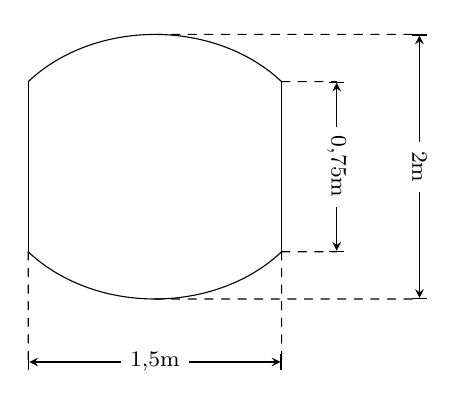
\begin{tikzpicture}[scale=0.7, font=\footnotesize, line join=round, line cap=round, >=stealth]
		\def\a{3}
		\def\b{2.4}
		\path
		(\a,0) coordinate (B)
		(140: \a cm and \b cm) coordinate (M)
		(40:\a cm and \b cm) coordinate (N)
		(-140:\a cm and \b cm) coordinate (Q)
		(-40:\a cm and \b cm) coordinate (P)
		(Q)+(0,-2) coordinate (Q1)
		(P)+(0,-2) coordinate (P1)
		(N)+(1,0) coordinate (N1)
		(P)+(1,0) coordinate (P2)
		(0,\b) coordinate (A)
		(0,-\b) coordinate (B)
		(A)+(4.8,0) coordinate (A1)
		(B)+(4.8,0) coordinate (B1)
		;
		\draw (M)--(Q) (N)--(P);
		\draw (N) arc (40:140:\a cm and \b cm);
		\draw (P) arc (-40:-140:\a cm and \b cm);
		\draw[dashed] (Q)--(Q1);
		\draw[dashed] (P)--(P1);
		\draw[|<->|,shift={(0,0)}] (Q1)--(P1) node[fill=white,midway]{$1{,}5$m};
		\draw[dashed] (A)--(A1);
		\draw[dashed] (B)--(B1);
		\draw[|<->|,shift={(1.8,0)}] (\a,-\b)--(\a,\b) node[fill=white,midway,rotate=-90]{$2$m};
		\draw[dashed] (N)--(N1);
		\draw[dashed] (P)--(P2);
		\draw[|<->|,shift={(1,0)}] (P2)--(N1) node[fill=white,midway,rotate=-90]{$0{,}75$m};
		\end{tikzpicture}}
	\loigiai{
		\begin{center}
			\begin{tikzpicture}[scale=1, font=\footnotesize, line join=round, line cap=round, >=stealth]
			\def\a{3.6}
			\def\b{2}
			\draw[->] (-5,0)--(5,0) node[below]{$x$};
			\draw[->] (0,-3)--(0,3) node[left]{$y$};
			\path
			(-\a,0) coordinate (A)
			(\a,0) coordinate (B)
			(0,\b) coordinate (C)
			(0,-\b) coordinate (D)
			(140: \a cm and \b cm) coordinate (M)
			(40:\a cm and \b cm) coordinate (N)
			(-140:\a cm and \b cm) coordinate (Q)
			(-40:\a cm and \b cm) coordinate (P)
			;
			\draw (M)--(Q) (N)--(P);
			\draw (N) arc (40:140:\a cm and \b cm);
			\draw (P) arc (-40:-140:\a cm and \b cm);
			\draw[dashed] (P) arc (-40:40:\a cm and \b cm);
			\draw[dashed] (M) arc (140:220:\a cm and \b cm);
			\foreach \p in {A,B,C,D,M,N,P,Q}
			\draw[fill=black] (\p) circle (1pt);
			\foreach \p/\g in {A/-120,B/-80,C/120,D/-120,M/100,N/80,P/-80,Q/-100}
			\path (\p)+(\g:3mm) node{$\p$}
			;
			\end{tikzpicture}
		\end{center}
		Để tính diện tích của phần gỗ ta cần dùng ý nghĩa hình học của tích phân.\\
		Đầu tiên ta cần lập phương trình đường Elip biểu thị bảng gỗ. Chọn hệ trục tọa độ $Oxy$ sao cho bảng gỗ này đối xứng qua $2$ trục $Ox$ và $Oy$.\\
		Theo số liệu đề cho ta có được các độ dài $CD = 1$ m, $MN = 1{,}5$ m, $NP = 0{,}75$ m.\\
		Đường Elip $\dfrac{x^2}{a^2}+\dfrac{y^2}{b^2}=1$ có trục nhỏ $CD = 1$m và đi qua điểm $N\left(\dfrac{3}{4};\dfrac{3}{8}\right)$, ta có
		$$\heva{&2b=1\\&\dfrac{\left(\dfrac{3}{4}\right)^2}{a^2}+\dfrac{\left(\dfrac{3}{8}\right)^2}{b^2}=1}\Leftrightarrow \heva{&b=\dfrac{1}{2}\\&a^2=\dfrac{9}{7}}\Rightarrow \dfrac{7}{9}x^2+4y^2=1\Rightarrow y=\pm \dfrac{1}{2}\sqrt{1-\dfrac{7}{9}x^2}.$$
		Diện tích gỗ cần có được tính theo công thức
		$$2\displaystyle\int\limits_{-0{,}75}^{0{,}75} \dfrac{1}{2}\sqrt{1-\dfrac{7}{9}x^2} \mathrm{\,d}x=\displaystyle\int\limits_{-0{,}75}^{0{,}75} \sqrt{1-\dfrac{7}{9}x^2} \mathrm{\,d}x\approx 1{,}4 \text{m}^2.$$
	}
\end{ex}

\begin{ex}%Câu 14.[Đỗ Đường Hiếu - ĐCHT THPT]%[2D3T3-7]
	\immini{Anh An muốn làm cửa rào sắt có hình dạng và kích thước giống như hình vẽ kế bên, biết đường cong phía trên là một parabol. Giá $1$m$^2$ cửa rào sắt có giá là $700000$ đồng. Vậy anh An phải trả bao nhiêu tiền để làm cài cửa rào sắt như vậy (làm tròn đến hàng nghìn)
		\choice
		{\True $6417000$ đồng}
		{$6320000$ đồng}
		{$6520000$ đồng}
		{$6620000$ đồng}}
	{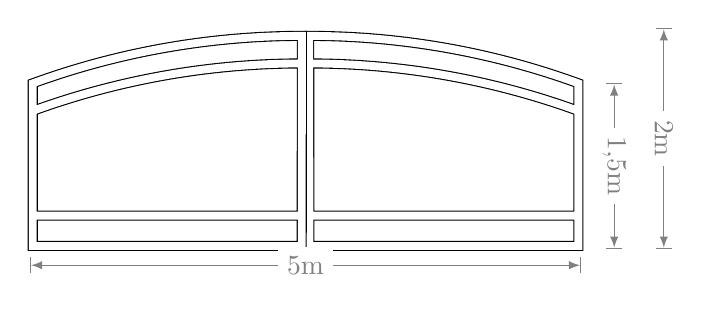
\begin{tikzpicture}[scale=0.7,>=latex]
		\draw[double,double distance=.1cm] (.07,.6)--(4.95,.6)(.07,.05)--(4.95,.05)--(4.95,3)arc(70:90:14.28)--cycle(4.95,2.5)arc(70:90:14.28);
		\draw[double,double distance=.1cm] (-.07,.6)--(-4.95,.6)(-.07,.05)--(-4.95,.05)--(-4.95,3)arc(110:90:14.28)--cycle(-4.95,2.5)arc(110:90:14.28);
		\draw[|<->|,gray,shift={(0,-.3)}] (-5,0)--(5,0) node[fill=white,midway]{$5$m};
		\draw[|<->|,gray,shift={(.6,0)}] (5,0)--(5,3) node[fill=white,midway,rotate=-90]{$1{,}5$m};
		\draw[|<->|,gray,shift={(1.5,0)}] (5,0)--(5,4) node[fill=white,midway,rotate=-90]{$2$m};
		%\draw[ultra thin,cyan](-5,0)grid(5,4);
		\end{tikzpicture}}
	\loigiai{
		\begin{center}
			\begin{tikzpicture}[scale=1, font=\footnotesize, line join=round, line cap=round, >=stealth]
			\def\a{2.5}
			\def\b{0.5}
			\draw[->] (-3.5,0)--(3.5,0) node[below]{$x$};
			\draw[->] (0,-3)--(0,2) node[left]{$y$};
			\path
			(0,0) coordinate (O)
			(-\a,0) coordinate (A)
			(\a,0) coordinate (B)
			(0,\b) coordinate (I)
			(\a,-1.5) coordinate (C)
			(-\a,-1.5) coordinate (D)
			;
			\draw (A) parabola bend (I) (B);
			\draw (A)--(D)--(C)--(B);
			\foreach \p in {A,B,C,D,I,O}
			\draw[fill=black] (\p) circle (1pt);
			\foreach \p/\g in {A/-120,B/-60,C/-80,D/-120,I/140,O/-130}
			\path (\p)+(\g:3mm) node{$\p$}
			;
			\path
			(\a,0) node[above]{$\a$}
			(-\a,0) node[above]{$-\a$}
			(0,\b) node[above right]{$\b$}
			(0,-1.5)node[below left]{$-1{,}5$}
			;
			\end{tikzpicture}
		\end{center}
		Ta mô hình hóa cánh cửa rào bằng hình thang cong $ADCB$ vuông tại $C$ và $D$, cung $AB$ như hình vẽ.\\
		Chọn hệ trục tọa độ $Oxy$ sao cho $2$ điểm $A$, $B$ nằm trên trục $Ox$ như hình vẽ.\\
		Vậy diện tích cánh cửa sẽ bằng diện tích hình chữ nhật $ABCD$ cộng thêm diện tích miền cong $AIB$. Để tính diện tích miền cong $AIB$ ta cần dùng tích phân.\\
		Đầu tiên ta tìm cách viết phương trình Parabol $y=ax^2+bx+c$ biểu thị cho đường cong $AIB$. Parabol có đỉnh $I\left(0;\dfrac{1}{2}\right)$ và cắt trục hoành tại $2$ điểm $A\left(-\dfrac{5}{2};0\right)$, $B\left(\dfrac{5}{2};0\right)$.\\
		Ta có
		$$\heva{&a\cdot 0^2+b\cdot 0+c=\dfrac{1}{2}\\&-\dfrac{b}{2a}=0\\&a\cdot \left(\dfrac{5}{2}\right)^2+b\cdot \left(\dfrac{5}{2}\right)+c=0}\Leftrightarrow \heva{&a=-\dfrac{2}{25}\\&b=0\\&c=\dfrac{1}{2}}\Rightarrow y=-\dfrac{2}{25}x^2+\dfrac{1}{2}.$$
		Diện tích miền cong $AIB$ được tính bằng công thức
		$$\displaystyle\int\limits_{-2{,}5}^{2{,}5} \left(-\dfrac{2}{25}x^2+\dfrac{1}{2}\right)\mathrm{\,d}x=\dfrac{5}{3}.$$
		Suy ra diện tích cánh cửa là $\dfrac{5}{3}+1{,}5\cdot 5=\dfrac{55}{6}$ m$^2$.\\
		Giá $1$m$^2$ cửa rào sắt giá $700000$.\\
		Vậy giá tiền cửa rào sắt là $6416666$.}
\end{ex}

\begin{ex}%Câu 15.[Đỗ Đường Hiếu - ĐCHT THPT]%[2D3T3-7]
	Trong một mẻ cấy, số lượng ban đầu của vi khuẩn là $500$, số lượng này tăng lên theo vận tốc $v(t)=450\mathrm{e}^{1{,}1257t}$ vi khuẩn trong $1$ giờ. Sẽ có bao nhiêu vi khuẩn trong buồng cấy sau $3$ giờ?
	\choice
	{\True $11807$}
	{$21600$}
	{$15809$}
	{$31250$}
	\loigiai{
		Gọi $S(t)$ là số lượng vi khuẩn trong buồng cấy sau $t$ giờ. Ta có $S(t)$ là nguyên hàm của hàm vận tốc $v(t)$
		$$S(t)=\displaystyle\int v(t)\mathrm{\,d}t=\displaystyle\int 450\mathrm{e}^{1{,}1257t}\mathrm{\,d}t=450\cdot\dfrac{1}{1{,}1257}\cdot \mathrm{e}^{1{,}1257t}+C.$$
		Số lượng vi khuẩn lúc ban đầu là $500$ con nên
		\begin{eqnarray*}
			&&S(0)=500\Leftrightarrow 450\cdot\dfrac{1}{1{,}1257}\cdot \mathrm{e}^{1{,}1257\cdot 0}+C =500\Leftrightarrow C=100{,}25;\\
			&&S(t)=450\cdot\dfrac{1}{1{,}1257}\cdot \mathrm{e}^{1{,}1257t}+100{,}25.
		\end{eqnarray*}
		Số vi khuẩn trong buồng cấy sau $3$ giờ
		$$S(3)=450\cdot\dfrac{1}{1{,}1257}\cdot \mathrm{e}^{1{,}1257\cdot 3}+100{,}25=11807.$$}
\end{ex}

\begin{ex}%Câu 16.[Đỗ Đường Hiếu - ĐCHT THPT]%[2D3T3-7]
	Chất điểm chuyển động theo một đường thẳng sau t giây đạt được vận tốc $v=t^2\cdot \mathrm{e}^{-t}$ m/s. Tính quãng đường nó đi được trong $t$ giây đầu tiên?
	\choice
	{$S(t)=2-\mathrm{e}^{-3t}\left(t^2+2t\right)$}
	{\True $S(t)=2-\mathrm{e}^{-t}\left(t^2+2t+2\right)$}
	{$S(t)=2-\mathrm{e}^{-t}\left(t^2+3t+2\right)$}
	{$S(t)=1-\mathrm{e}^{-t}\left(5t^2+2t+2\right)$}
	\loigiai{
		Gọi $S(t)$ là quãng đường chất điểm đi được sau $t$ giây đầu tiên. Ta có $S(t)$ là nguyên hàm của vận tốc $v=t^2\cdot \mathrm{e}^{-t}$ m/s.\\
		$$S(t)=\displaystyle\int v(t)\mathrm{\,d}t=\displaystyle\int \left( t^2\cdot \mathrm{e}^{-t}\right) \mathrm{\,d}t.$$
		Dùng phương pháp nguyên hàm từng phần ta tính được
		$$S(t)=\displaystyle\int v(t)\mathrm{\,d}t=\displaystyle\int \left( t^2\cdot \mathrm{e}^{-t}\right) \mathrm{\,d}t=2-\mathrm{e}^{-t}\left(t^2+2t+2\right).$$}
\end{ex}

\begin{ex}%Câu 17.[Đỗ Đường Hiếu - ĐCHT THPT]%[2D3T3-7]
	Công ty vừa đưa vào một dây chuyền sản xuất để chế tạo máy tính mới. Sau vài tuần, sản lượng đạt được $q(t)=4000\left(1-\dfrac{10}{(10-t)^2}\right)$ máy/tuần. Tìm số máy sản xuất được từ tuần thứ ba đến hết tuần thứ tư. 
	\choice
	{$45000$}
	{$5235$}
	{\True $6333$}
	{$5315$}
	\loigiai{
		Số lượng máy tính từ đầu tuần thứ $3$ đến hết tuần thứ $4$ là 
		$$\displaystyle\int\limits_{2}^{4} 4000\left(1-\dfrac{10}{10-t^2}\right)\mathrm{\,d}t=4000t\bigg|_2^4+\dfrac{40000}{t-10}\bigg|_2^4\approx 6333.$$}
\end{ex}

\begin{ex}%Câu 18.[Đỗ Đường Hiếu - ĐCHT THPT]%[2D3T3-7]
	Người ta dự đoán rằng dân số thay đổi với tốc độ $\mathrm{e}^{0{,}001t}$ (tỷ người/năm) với $t$ là số năm tính từ năm $2003$. Biết rằng năm $2009$ dân số thế giới là $4{,}5$ (tỷ người). Dân số thế giới vào năm $2013$ vào khoảng
	\choice
	{$9{,}03$ tỷ người}
	{$8{,}65$ tỷ người}
	{$8{,}53$ tỷ người}
	{\True $9{,}54$ tỷ người}
	\loigiai{
		Gọi $P(t)$ là dân số thế giới sau $t$ năm tính từ $2003$.\\
		Khi ấy theo đề ra ta có $P'(t)=\mathrm{e}^{0{,}001t}$. Suy ra
		$$P(t)=\displaystyle\int P'(t)\mathrm{\,d}t=\displaystyle\int \mathrm{e}^{0{,}001t}\mathrm{\,d}t=\dfrac{1}{0{,}001}\mathrm{e}^{0{,}001t}+C=1000\mathrm{e}^{0{,}001t}+C.$$
		Dân số năm $2009$ (ứng với $t =$) là $4{,}5$ tỷ người nên
		$$P(6)=4{,}5\Leftrightarrow 1000\mathrm{e}^{0{,}001\cdot 6}+C=4{,}5\Leftrightarrow C=4{,}5-1000\mathrm{e}^{0{,}006}.$$
		Do đó $P(t)=1000\mathrm{e}^{0{,}001t}+4{,}5-1000\mathrm{e}^{0{,}006}$.\\
		Suy ra $P(11)=1000\mathrm{e}^{0{,}001\cdot 11}+4{,}5-1000\mathrm{e}^{0{,}006}\approx 9{,}54$.\\
		Vậy dân số thế giới năm $2013$ là $9{,}54$ (tỷ người).}
\end{ex}

\begin{ex}%Câu 19.[Đỗ Đường Hiếu - ĐCHT THPT]%[2D3T3-7]
	Tốc độ thay đổi số dân của một thị trấn kể từ năm $1970$ được mô tả bằng công thức $f'(t)=\dfrac{120}{(t+5)^2}$, với $t$ là thời gian tính bằng năm (thời điểm $t = 0$ ứng với năm $1970$). Biết rằng số dân của thị trấn vào năm $1970$ là $2000$ người. Hỏi số dân của thị trấn đó vào năm $2008$ ước tính là bao nhiêu?
	\choice
	{$32{,}1$ nghìn người}
	{\True $23{,}21$ nghìn người}
	{$15{,}32$ nghìn người}
	{$20{,}41$ nghìn người}
	\loigiai{
		Tốc độ thay đổi số dân của thị trấn vào năm thứ $t$ là $f'(t)=\dfrac{120}{(t+5)^2}$. Suy ra nguyên hàm của $f'(t)$ là hàm số $f(t)$ mô tả số dân của thị trấn vào năm thứ $t$. Ta có
		$$f(t)=\displaystyle\int f'(t)\mathrm{\,d} t=\displaystyle\int \dfrac{120}{(t+5)^2}\mathrm{\,d} t=\dfrac{-120}{t+5}+C.$$
		Số dân của thị trấn vào năm $1970$ (ứng với $t = 0$) là
		\begin{eqnarray*}
			f(0)=2&\Leftrightarrow& \dfrac{-120}{0+5}+C=2\Leftrightarrow C=26\\
			&\Rightarrow& f(t)=\dfrac{-120}{t+5}+26.
		\end{eqnarray*}
		Vậy số dân của thị trấn vào năm $2008$ (ứng với $t = 38$) là
		$f(28)=\dfrac{-120}{38+5}+26=23{,}21$ ngàn người.}
\end{ex}

\begin{ex}%Câu 20.[Đỗ Đường Hiếu - ĐCHT THPT]%[2D3T3-7]
	Hưởng ứng phong trào \lq\lq Ngày vì người nghèo\rq\rq\, do Đài truyền hình Việt Nam tổ chức, tối ngày 10/04/2010 chương trình  \lq\lq Góp sức vì người nghèo\rq\rq\, đã được tổ chức tại $3$ điểm cầu truyền hình tại $3$ thành phố lớn của cả nước là TP Hà Nội, TP Đà Nẵng, TP Hồ Chí Minh và được truyền hình trực tiếp trên sóng VTV3 – Đài truyền hình Việt Nam. Trong chương trình này, các cá nhân tổ chức trong và ngoài nước sẽ có dịp được chung tay góp sức giúp đỡ cho người nghèo qua hình thức nhắn tin hoặc quyên góp tiền trực tiếp cho ban tổ chức chương trình. Theo ước tính, sau $t$ (giờ) số tiền quyên góp thay đổi với tốc độ $300 t\cdot\mathrm{e}^{-0{,}1t}$ (triệu đồng/giờ). Số tiền có được sau $5$ giờ đầu tiên quyên góp là 
	\choice
	{$321$ triệu đồng}
	{$3209$ triệu đồng}
	{\True $2706{,}12$ triệu đồng}
	{$9801$ triệu đồng}
	\loigiai{
		Gọi $M(t)$ là số tiền có được sau $t$ (giờ) thực hiện việc quyên góp.\\
		Khi ấy theo đề ta có $M'(t)=300 t\cdot\mathrm{e}^{-0{,}1t}$. Suy ra
		$$M(t)=\displaystyle\int M'(t)\mathrm{\,d}t=\displaystyle\int 300 t\cdot\mathrm{e}^{-0{,}1t}\mathrm{\,d}t.$$
		Đặt $\heva{&u=300t\\&\mathrm{\,d}v=\mathrm{e}^{-0{,}1t}\mathrm{\,d}t}\Rightarrow \heva{&\mathrm{\,d}u=300\mathrm{\,d}t\\&v=-10\mathrm{e}^{-0{,}1t}.}$\\
		Suy ra 
		$$M(t)=-3000t\cdot \mathrm{e}^{-0{,}1t}+\displaystyle\int 3000\cdot\mathrm{e}^{-0{,}1t}\mathrm{\,d}t=-3000t\cdot \mathrm{e}^{-0{,}1t}-30000\cdot \mathrm{e}^{-0{,}1t}+C.$$		
		Lúc ban đầu ($t = 0$) thì số tiền quyên góp là
		$$M(0)=0\Leftrightarrow -3000\cdot 0\cdot \mathrm{e}^{-0{,}1\cdot 0}-30000\cdot \mathrm{e}^{-0{,}1\cdot 0}+C=0\Leftrightarrow C=30000.$$
		Do đó $M(t)=-3000t\cdot \mathrm{e}^{-0{,}1t}-30000\cdot \mathrm{e}^{-0{,}1t}+30000$.\\
		Sau $5$ giờ số tiền quyên góp được là 
		$$M(5)=-3000\cdot 5\cdot \mathrm{e}^{-0{,}1\cdot 5}-30000\cdot \mathrm{e}^{-0{,}1\cdot 5}+30000\approx 2706{,}12\;(\text{triệu đồng}).$$}
\end{ex}

\begin{ex}%Câu 21.[Đỗ Đường Hiếu - ĐCHT THPT]%[2D3T3-7]
	Việc thở là những vòng tuần hoàn, mỗi vòng tính từ lúc bắt đầu hít vào đến lúc kết thúc thở ra, thường kéo dài trong $5$s. Vận tốc cực đại của khí là $V$ l/s,vì thế nó được mô hình hoá bởi $v(t)=V\sin \dfrac{2\pi t}{5}$. Tính thể tích khí hít vào phổi sau thời gian $2$s. 
	\choice
	{$2{,}5V$ lít}
	{\True $1{,}44V$ lít}
	{$2V$ lít}
	{$3{,}6V$ lít}
	\loigiai{
		Vận tốc của khí hít vào được mô hình bởi công thức $v(t)=V\sin \dfrac{2\pi t}{5}$. Suy ra lượng khí hít vào sau $2$ giây là 
		$$N(2)=\displaystyle\int\limits_0^2 v(t)\mathrm{\,d}t=\displaystyle\int\limits_0^2 V\sin \dfrac{2\pi t}{5}\mathrm{\,d}t=\dfrac{5V}{2\pi}\left(1-\cos\dfrac{2\pi\cdot 2}{5}\right)=1{,}44\;(\text{lít khí}).$$}
\end{ex}

\begin{ex}%Câu 22.[Đỗ Đường Hiếu - ĐCHT THPT]%[2D3T3-7]
	Giả sử rằng sau $t$ năm, vốn đầu tư của một doanh nghiệp phát sinh lợi nhuận với tốc độ $P'(t)=126+t^2$ (triệu đồng/năm). Hỏi sau $10$ năm đầu tiên thì doanh nghiệp thu được lợi nhuận là bao nhiêu (đơn vị triệu đồng)?
	\choice
	{\True $\dfrac{4780}{3}$}
	{$1235$}
	{$\dfrac{3257}{3}$}
	{$5020$}
	\loigiai{
		Gọi $P(t)$ là lợi nhuận phát sinh của vốn sau $t$ năm đầu tư. Ta có $P(t)$ là nguyên hàm của hàm tốc độ $P'(t)$.\\
		Lợi nhuận phát sinh sau 10 năm đầu tiên là
		$$\displaystyle\int\limits_0^{10} P'(t)\mathrm{\,d}t=\displaystyle\int\limits_0^{10} \left(126+t^2\right) \mathrm{\,d}t=\dfrac{4780}{3}\;\left( \text{triệu đồng}\right) $$.}
\end{ex}

\begin{ex}%Câu 23.[Đỗ Đường Hiếu - ĐCHT THPT]%[2D3T3-7]
	Một vật chuyển động chậm dần với vận tốc $v(t)=150-10t $(m/s). Hỏi rằng trong $4$s trước khi dừng hẳn vật di chuyển được bao nhiêu mét?
	\choice
	{$15$ m}
	{$520$ m}
	{\True $80$ m}
	{$125$ m}
	\loigiai{
		Vật chuyển động chậm dần cho đến khi dừng hẳn thì
		$$v(t)=0 \Leftrightarrow 150-10t=0 \Leftrightarrow t=15(\text{s}).$$
		Quãng đường vật đi được từ giây thứ $13$ đến giây thứ $16$ là
		$$S=\displaystyle\int\limits_{11}^{15} v(t)\mathrm{\,d}t=\displaystyle\int\limits_{11}^{15}(150-10t)\mathrm{\,d}t=80\;(\text{m}).$$}
\end{ex}

\begin{ex}%Câu 24.[Đỗ Đường Hiếu - ĐCHT THPT]%[2D3T3-7]
	Một vật chuyển động với gia tốc $a(t)=\dfrac{2}{t+2}$ (m/s$^2$). Vận tốc ban đầu của vật là $7$m/s. Hỏi vận tốc của vật tại giây thứ $5$ bằng bao nhiêu?
	\choice
	{$3{,}89$ (m/s)}
	{\True $9{,}51$ (m/s)}
	{$7{,}38$ (m/s)}
	{$10{,}89$ (m/s)}
	\loigiai{
		Vận tốc của vật tại thời điểm t được tính theo công thức
		$$v(t)=\displaystyle\int a(t)\mathrm{\,d}t=\displaystyle\int \dfrac{2}{t+2}\mathrm{\,d}t=2\ln |t+2|+C.$$
		Vì vận tốc ban đầu (lúc $t=0$) của vật là $v_0=6$ m/s nên
		$$v(0)=2\ln |0+2|+C=7 \Leftrightarrow C=7-2\ln 2 \Rightarrow v(t)=2\ln |t+2|+7-2\ln 2.$$
		Vận tốc của vật chuyển động tại giây thứ $5$ là
		$v(5)=2\ln |5+2|+7-2\ln 2\approx 9,51$ m/s.}
\end{ex}

\begin{ex}%Câu 25.[Đỗ Đường Hiếu - ĐCHT THPT]%[2D3T3-7]
	Một học sinh tự chế tên lửa và phóng tên lửa từ mặt đất với vận tốc ban đầu là $30$ m/s. Giả sử bỏ qua sức cản của gió, tên lửa chỉ chịu tác động của trọng lực. Độ cao lớn nhất mà tên lửa có thể đạt được là (biết rằng gia tốc rơi tự do là $g=9{,}8$ m/s$^2$).
	\choice
	{$\dfrac{5250}{49}$ m}
	{$\dfrac{52500}{49}$ m}
	{\True $\dfrac{2250}{49}$ m}
	{$\dfrac{22500}{49}$ m}
	\loigiai{
		Độ cao của tên lửa là nguyên hàm của vận tốc, suy ra
		$$s(t)=\displaystyle\int v(t)\mathrm{\,d}t=\displaystyle\int (-9,8t+30)\mathrm{\,d}t=-4,9t^2+30t+C_2.$$
		Vì $s(0)=0$ nên $s(0)=-4,9.0^2+30.0+C_2=0 \Leftrightarrow C_2=0 \Rightarrow s(t)=-4,9t^2+30t$.\\
		Đồ thị của hàm số $s(t)=-4,9t^2+30t$ là đường cong Parabol có đỉnh $I\left(\dfrac{150}{49} ;\dfrac{2250}{49}\right)$ nên tên lửa đạt độ cao lớn nhất là $\dfrac{2250}{49}$ (m) tại thời điểm $t=\dfrac{150}{49}$ (s).}
\end{ex}

\begin{ex}%Câu 26.[Đỗ Đường Hiếu - ĐCHT THPT]%[2D3T3-7]
	Vi khuẩn HP (Helicobacter pylori) gây đau dạ dày tại ngày thứ $t$ với số lượng là $F(t)$, biết nếu phát hiện sớm khi số lượng vi khuẩn không vượt quá $5000$ con thì bệnh nhân sẽ được cứu chữa. Biết tốc độ phát triển của vi khuẩn tại ngày thứ $t$ là $F'(t)=\dfrac{1000}{t+1}$ và ban đầu bệnh nhân có $2000$ con vi khuẩn. Sau $10$ ngày bệnh nhân phát hiện ra bị bệnh. Hỏi khi đó có bao nhiêu con vi khuẩn trong dạ dày (lấy xấp xỉ hàng thập phân thứ hai) và bệnh nhân có cứu chữa được không?
	\choice
	{$5433{,}99$ và không cứu được}
	{\True $5044{,}52$ và không cứu được}
	{$4320{,}01$ và cứu được}
	{$2397{,}89$ và cứu được}
	\loigiai{
		Tốc độ phát triển của vi khuẩn tại ngày thứ $t$ là $F'(t)=\dfrac{1000}{t+1}$. Suy ra số lượng vi khuẩn vào ngày thứ t được tính theo công thức
		$$F(t)=\displaystyle\int F'(t)\mathrm{\,d}t=\displaystyle\int \dfrac{1000}{t+1}\mathrm{\,d}t=1000\ln |t+1|+C=1000\ln |t+1|+C.$$
		Lúc ban đầu bệnh nhân có $2000$ con vi khuẩn nên
		\begin{eqnarray*}
			F(0)=2000& \Leftrightarrow& 1000\ln |2.0+1|+C=2000 \Leftrightarrow C=2000 \\
			&  \Rightarrow &F(t)=1000\ln |t+1|+2000.
		\end{eqnarray*}
		Số vi khuẩn sau 10 ngày là $F(10)=1000\ln |2.10+1|+2000=5044,52$ con và bệnh nhân không cứu được.}
\end{ex}

\begin{ex}%Câu 27.[Đỗ Đường Hiếu - ĐCHT THPT]%[2D3T3-7]
	Một ô tô đang chuyển động với vận tốc $12$ m/s thì người lái xe bất ngờ tăng tốc cho xe chạy nhanh dần đều, sau $15$ s thì xe đạt vận tốc $15$m/s. Tính quãng đường xe đi được sau $30s$ 
	kể từ khi tăng tốc.
	\choice
	{$270$ m}
	{\True $450$ m}
	{$360$ m}
	{$540$ m}
	\loigiai{
		Ta có sau $15$s thì xe đạt vận tốc $15$ m/s (áp dụng $v=v_0+at$).\\
		Suy ra $15=12+a\cdot 15 \Rightarrow a=\dfrac{1}{5}=0{,}2$ (m/s$^2$)\\
		Vận tốc mà xe đạt sau $30$s là $v=12+0{,}2t$.\\
		Vậy quãng đường xe đi được sau khi tăng tốc $30$ s là $S=\displaystyle\int\limits_0^{30}(12+0{,}2t)\mathrm{\,d}t=450$ m.}
\end{ex}
\begin{ex}%[Dự án TLDH3-Nhóm Latex, Kiều Ngân]%[2D3K3-7]%Câu 27.
	Một ô tô đang chuyển động với vận tốc $12$ m/s thì người lái xe bất ngờ tăng tốc cho xe chạy nhanh dần đều, sau $15$ s thì xe đạt vận tốc $15$ m/s. Tính quãng đường xe đi được sau $30$ s 
	kể từ khi tăng tốc
	\choice
	{$270$ m}
	{\True $450$ m}
	{$360$ m}
	{$540$ m}
	\loigiai{
		Ta có sau $15$ s thì xe đạt vận tốc $15$ m/s (áp dụng $v=v_0+at$) $\Rightarrow 15=12+a\cdot 15 \Rightarrow a=\dfrac{1}{5}=0{,}2\left(\text{m/s}^2\right)$\\
		Vận tốc mà xe đạt sau $30$ s là $v=12+0{,}2t$.\\
		Vậy quãng đường xe đi được sau khi tăng tốc $30$ s là $S=\displaystyle\int\limits_0^{30}(12+0{,}2t)\mathrm{\,d}t=450$ m.}
\end{ex}
\begin{ex}%[Dự án TLDH3-Nhóm Latex, Kiều Ngân]%[2D3K3-7]%Câu 28.
	Một lực có độ lớn $40$ N (Newton) cần thiết để kéo căng một chiếc lò xo có độ dài tự nhiên $10$ cm lên $15$ cm. Biết rằng theo định luật Hooke trong Vật lý, khi một chiếc lò xo bị kéo căng thêm $x$ (đơn vị độ dài) so với độ dài tự nhiên của lò xo thì lò xo trì lại (chống lại) với một lực cho bởi công thức $f(x)=kx$ (N), trong đó $k$ là hệ số đàn hồi (hoặc độ cứng) của lò xo. Hãy tìm công sinh ra khi kéo lò xo có độ dài từ $15$ cm đến $20$ cm? (kí hiệu J (Jun) là đơn vị của công).
	\choice
	{\True $3{,}00$ J}
	{$1{,}56$ J}
	{$2{,}56$ J}
	{$3{,}18$ J}
	\loigiai{
		Khi kéo lò xo từ $10$ cm đến $15$ cm nó bị kéo căng thêm $5$ cm $= 0{,}05$ m.\\
		Suy ra $f(0{,}05)=40 \Leftrightarrow 0{,}05k=40 \Rightarrow k=800$. Do đó $f(x)=800x$.\\
		Công được sinh ra khi kéo căng lò xo từ $15$ cm đến $20$ cm là $W=\displaystyle\int\limits_{0{,}05}^{0{,}1} f(x)\mathrm{\,d}x$\\
		$\Rightarrow W=\displaystyle\int\limits_{0{,}05}^{0{,}1} f(x)\mathrm{\,d}x=\displaystyle\int\limits_{0{,}05}^{0{,}1}(800x)\mathrm{\,d}x=800\left(\dfrac{x^2}{2}\right)\bigg|_{0{,}05}^{0{,}1}=3$ (J).}
\end{ex}
\begin{ex}%[Dự án TLDH3-Nhóm Latex, Kiều Ngân]%[2D3K3-7]%Câu 29.
	Công ty vừa đưa vào một dây chuyền sản xuất để chế tạo máy tính mới. Sau vài tuần, sản lượng đạt được $q(t)=2000\left(1-\dfrac{10}{(10-t)^2}\right)$ máy/tuần. Tìm số máy sản xuất được từ tuần thứ ba đến hết tuần thứ tư. 
	\choice
	{$147$ máy}
	{\True $1523$ máy}
	{$1470$ máy}
	{$3166$ máy}
	\loigiai{
		Số lượng máy tính từ đầu tuần thứ $3$ đến hết tuần thứ $4$ là $\displaystyle\int\limits_3^4 2000\left(1-\dfrac{10}{(10-t)^2}\right)\mathrm{\,d}t=1523$.}
\end{ex}
\begin{ex}%[Dự án TLDH3-Nhóm Latex, Kiều Ngân]%[2D3K3-7]%Câu 30.
	Việc thở là những vòng tuần hoàn, mỗi vòng tính từ lúc bắt đầu hít vào đến lúc kết thúc thở ra, thường kéo dài trong $5$ s. Vận tốc cực đại của khí là $V$ l/s, vì thế nó được mô hình hoá bởi $v(t)=V\sin \dfrac{3\pi t}{5}$. Tính thể tích khí hít vào phổi sau thời gian $2$ s. 
	\choice
	{$0{,}02V$ (lít)}
	{\True $1{,}06V$ (lít)}
	{$0{,}95V$ (lít)}
	{$3{,}12V$ (lít)}
	\loigiai{
		Vận tốc của khí hít vào được mô hình bởi công thức $v(t)=V\sin \dfrac{3\pi t}{5}$. Suy ra lượng khí hít vào sau $2$ giây là
		$$N(2)=\displaystyle\int\limits_0^2 v(t)\mathrm{\,d}t=\displaystyle\int\limits_0^2 V\sin \dfrac{3\pi t}{5}\mathrm{\,d}t=\dfrac{5V}{3\pi }\left(1-\cos \dfrac{3\pi \cdot 2}{5}\right)=1{,}06V \text{ (lít).}$$}
\end{ex}
\begin{ex}%[Dự án TLDH3-Nhóm Latex, Kiều Ngân]%[2D3K3-7]%Câu 31.
	Một chiếc xe thể thao hiệu Lamborghini Aventador chạy trên một đường đua thẳng có độ dài $4$ km. Xe tăng tốc từ $0$ km/h đến $100$ km/h trong $3$ giây đầu tiên đi hết $260$ m và sau đó xe chuyển động nhanh dần đều với gia tốc $20$ m/s. Tính thời gian để xe hoàn thành đường đua biết vận tốc của chuyển động nhanh dần đều có công thức $v=at+v_0$ với $a$, $v_0$ là gia tốc và vận tốc đầu. 
	\choice
	{\True $18$ s}
	{$21$ s}
	{$11$ s}
	{$14$ s}
	\loigiai{
		Ta có $100$ km/h $=\dfrac{250}{9}$ m/s, vận tốc nhanh dần đều là $v=20t+\dfrac{250}{9}$.\\
		Gọi $t_0$ là thời gian xe hoàn thành $4000-260=3740$ m còn lại.\\
		Ta có $S=\displaystyle\int\limits_0^{t_0}\left(20t+\dfrac{250}{9}\right)\mathrm{d}t=\left(10t^2+\dfrac{250}{9} t\right)\bigg|_0^{t}=10t_0^2+\dfrac{250}{9} t_0$.\\
		Suy ra $10t_{0}^2+\dfrac{250}{9} t_{0}=3740 \Leftrightarrow \hoac{&t_{0}=18 \\& t_{0}=-\dfrac{187}{9}\text{ (loại)}} \Rightarrow t_{0}=18\text{ s}$.}
\end{ex}
\begin{ex}%[Dự án TLDH3-Nhóm Latex, Kiều Ngân]%[2D3K3-7]%Câu 32.
	Một vật đang chuyển động thẳng nhanh dần đều có vận tốc là $18$ km/h. Trong giây thứ $5$ vật đi được quãng đường là $5{,}9$ m, tính quãng đường vật đi được sau $10$ s kể từ lúc bắt đầu chuyển động.
	\choice
	{$\dfrac{132}{5}$ m}
	{$103{,}6$ }
	{\True $60$ m}
	{$\dfrac{121}{3}$ m}
	\loigiai{
		Ta có $18$ km/h $=\dfrac{18}{3{,}6}=5$ m/s. Quãng đường vật đi được trong khoảng thời gian $t$ là $S=v_0 t+\dfrac{at^2}{2}$.\\
		Vậy trong giây thứ $5$ quãng đường nó đi được là $$\Delta S=5\cdot 5+\dfrac{a\cdot 5^2}{2}-5\cdot 4-\dfrac{a\cdot 4^2}{2}=5{,}9 \Rightarrow a=0{,}2 \text{ m/s}^2.$$
		Vậy quãng đường mà vật đi được sau $10$ s kể từ lúc bắt đầu chuyển động là
		$S=\displaystyle\int\limits_0^{10}(5+0{,}2t)\mathrm{\,d}t=60$ m.}
\end{ex}

\begin{ex}%[Dự án TLDH3-Nhóm Latex, Kiều Ngân]%[2D3K3-7]%Câu 34.
	Một mạch kín gồm một nguồn điện có suất điện động biến thiên theo thời gian $e=10\cos (100\pi t)$ (V) và điện trở trong không đáng kể, nối với mạch ngoài có một điện trở $R=50$ $\Omega$. Tính điện lượng chuyển qua điện trở trong thời gian từ $t=0$ đến $t=\dfrac{1}{600}$ s.
	\choice
	{\True $3{,}18\cdot 10^{-5}$ C}
	{$15{,}9$ $\mu$C}
	{$3{,}18$ nC}
	{$1{,}59$ nC}
	\loigiai{
		Ta có $i=\dfrac{u}{R}=0{,}02\cos (100\pi t)$ (A). Ta có $i(t)=q'(t)$.\\
		Do đó $q=\displaystyle\int\limits_{t_1}^{t_2} i(t)\mathrm{\,d}t$. Xét điện lượng từ $t=0$ đến $t=\dfrac{1}{600}$ s, ta có
		$$q=0{,}02\displaystyle\int\limits_0^{\tfrac{1}{600}}\cos (100\pi t)\mathrm{\,d}t=3{,}18\cdot 10^{-5}\text{ C}.$$}
\end{ex}
\begin{ex}%[Dự án TLDH3-Nhóm Latex, Kiều Ngân]%[2D3K3-7]%Câu 35.
	Một hạt proton di chuyển trong điện trường có biểu thức gia tốc (theo m/s$^2$) là $a=-\dfrac{20}{(2t+1)^2}$ với $t$ tính bằng giây. Tìm hàm vận tốc $v$ theo $t$, biết rằng $t=0$ thì $v=40$ m/s. 
	\choice
	{$v(t)=30+\dfrac{10}{2t+1}$ (m/s)}
	{\True $v(t)=20+\dfrac{10}{2t+1}$ (m/s)}
	{$v(t)=30+\dfrac{20}{2t+1}$ (m/s)}
	{$v(t)=20+\dfrac{30}{2t+1}$ (m/s)}
	\loigiai{
		Ta có $v=\displaystyle\int a(t)\mathrm{\,d}t=\displaystyle\int \dfrac{-20}{(2t+1)^2}\mathrm{\,d}t=\dfrac{10}{2t+1}+C$.\\
		Khi $t=0 \Rightarrow v(0)=30 \Leftrightarrow \dfrac{10}{1+2.0}+C=40 \Leftrightarrow C=30$.\\
		Do đó biểu thức vận tốc theo thời gian là $v(t)=20+\dfrac{10}{2t+1}$ (m/s).}
\end{ex}
\begin{ex}%[Dự án TLDH3-Nhóm Latex, Kiều Ngân]%[2D3K3-7]%Câu 36.
	Trong mạch điện của thiết bị điện tử, cường độ dòng điện (đơn vị mA) là một hàm số theo thời gian $t$ là $i(t)=0{,}3-0{,}2t$ (mA). Tổng điện tích đi qua một điểm trong mạch trong giây $0{,}05$ s là bao nhiêu, biết rằng tại thời điểm ban đầu thì lượng điện tích chạy qua dây dẫn bằng $0$?
	\choice
	{$0{,}015$ mC}
	{\True $0{,}015$ $\mu$C}
	{$0{,}03$ $\mu$C}
	{$0{,}03$ mC}
	\loigiai{
		Ta biết rằng cường độ dòng diện là lượng điện tích đi qua tiết diện vật dẫn trong một đơn vị thời gian. Nếu gọi hàm $i(t)$ biểu thị cho cường độ dòng điện thì lượng điện tích $q(t)$ là nguyên hàm của $i(t)$.\\
		Ta có biểu thức điện tích $q(t)=\displaystyle\int i(t)\mathrm{\,d}t=\displaystyle\int (0,3-0,2t)\mathrm{\,d}t=0{,}3t-0{,}1t^2+C$.\\
		Ta có khi $q(0)=0 \Leftrightarrow C=0$. Do đó tổng điện tích đi qua một điểm trong $0{,}05$ s là 
		$$q(0{,}05)=0{,}3\cdot (0{,}05)-0{,}1\cdot (0{,}05)^2=0{,}015 \text{ $\mu$C}.$$}
\end{ex}
\begin{ex}%[Dự án TLDH3-Nhóm Latex, Kiều Ngân]%[2D3K3-7]%Câu 37.
	Hiệu điện thế đi qua tụ điện có điện dung $C=8,5$ nF đặt trong mạch thu sóng FM gần bằng $0$. Nếu có cường độ dòng điện $i=0{,}042t$ (mA) nạp vào tụ. Tìm hiệu điện thế sau $2\mu s$, biết rằng hiệu điện thế tại thời điểm $t$ được tính theo công thức $U(t)=\dfrac{q(t)}{C}$ với $q(t)$ là điện lượng qua tiết diện dây dẫn trong thời gian $t$. 
	\choice
	{$4{,}941$ nV}
	{$3{,}294$ nV}
	{$13{,}18$ nV}
	{\True $9{,}882$ nV}
	\loigiai{
		Lưu ý $1$ nF $=10^-9$ F, $1$ $\mu$s $=10^{-6}$ s.\\
		Ta biết rằng điện tích $q(t)$ là nguyên hàm của cường độ dòng điện $i(t)$.\\
		Ta có $U_C=\dfrac{1}{C}\displaystyle\int i(t)\mathrm{\,d}t=\dfrac{0{,}042\cdot 10^{-3}}{8{,}5\cdot 10^{-9}}\displaystyle\int t\mathrm{\,d}t=\left(\dfrac{4{,}94\cdot 10^3}{2}\right)t^2+K$.\\
		Theo giả thiết ta có $U(0)=0\Leftrightarrow K=0$.\\
		Do đó $U_C(t)=2{,}47\cdot 10^3 t^2$.\\
		Khi đó $U_C(2\mu s)=2{,}47\cdot 10^3(2\cdot 10^{-6})^2=9{,}882\cdot 10^{-9}=9{,}882$ nV.}
\end{ex}
\begin{ex}%[Dự án TLDH3-Nhóm Latex, Kiều Ngân]%[2D3K3-7]%Câu 38.
	Một lực $12$ N nén lò xo từ chiều dài tự nhiên là $18$ cm xuống còn $16$ cm. Hỏi công sinh ra là bao nhiêu nếu ta tiếp túc nén lò xo từ $16$ cm xuống $14$ cm?
	\choice
	{\True $3{,}6$ N}
	{$1{,}8$ N}
	{$0{,}9$ N}
	{$1{,}2$ N}
	\loigiai{
		Đầu tiên ta sẽ xác định hằng số lò xo (theo đơn vị m).\\
		Ta có $F=kx\Leftrightarrow 12=k(18-16)\cdot 10^{-2}\Rightarrow k=600$ N/m.\\
		Do đó ta có $F=600x$. Nên công sinh ra được xác định $A=\displaystyle\int\limits_{0{,}02}^{0{,}04} f(x)\mathrm{\,d}x=\displaystyle\int\limits_{0{,}02}^{0{,}04} 600x\mathrm{\,d}x$.\\
		Suy ra $A=300(x^2)\bigg|_{0{,}02}^{0{,}04}=3{,}6$ N.}
\end{ex}
\begin{ex}%[Dự án TLDH3-Nhóm Latex, Kiều Ngân]%[2D3K3-7]%Câu 39.
	Một người đi xe môtô với độ tăng vận tốc tại một thời điểm $t$ (tính theo giây, $t\ge 0$) được cho bởi hàm số $f(t)=\dfrac{1}{300}t^2+\dfrac{1}{1350}t$ (km/s$^2$). Nếu bắt đầu tăng tốc tính từ lúc khởi động máy (vận tốc bằng $0 $km/h), hỏi mất bao lâu thì người đó đạt đến tốc độ $120$ km/h?
	\choice
	{\True $3$ giây}
	{$3{,}05$ giây}
	{$47{,}5$ giây}
	{$189{,}63$ giây}
	\loigiai{
		Gọi $x$ là thời gian cần thiết để người đó đạt đến tốc độ $120$ km/h.\\
		Ta nhận xét độ tăng vận tốc trong thời gian này cũng chính là tích phân của hàm $f(t)$ với $t = 0$ đến $t = x$. Như vậy ta xét phương trình sau
		\begin{eqnarray*}
			&&\displaystyle\int\limits_0^x\left(\dfrac{1}{300}t^2+\dfrac{1}{1350}t\right)\mathrm{\,d}t=\dfrac{120}{3600}\\
			&\Leftrightarrow& \left(\dfrac{1}{900}t^3+\dfrac{1}{2700}t^2\right)\bigg|_0^x=\dfrac{1}{30}\\
			&\Leftrightarrow& \dfrac{1}{900}x^3+\dfrac{1}{2700}x^2=\dfrac{1}{30}\Leftrightarrow x=3 \text{ (s).}
		\end{eqnarray*}
	}
\end{ex}
\begin{ex}%[Dự án TLDH3-Nhóm Latex, Kiều Ngân]%[2D3K3-7]%Câu 40.
	Hai người chạy đua xuất phát cùng lúc với vận tốc $0$ m/s trên một đoạn đường $400$ m. Biết độ tăng vận tốc của $2$ người lần lượt cho bởi hai hàm số $f(t)=\dfrac{3}{100}t+\dfrac{1}{10}$ (m/s$^2$) và $g(t)=\dfrac{8}{25}$ (m/s$^2$) ($t$ là thời gian, tính theo giây). Hỏi thời gian về đích của hai người chênh lệch bao nhiêu giây?
	\choice
	{$8$ giây}
	{\True $10$ giây}
	{$40$ giây}
	{$1090$ giây}
	\loigiai{
		Ta nhận xét nguyên hàm của $f(t)$ và $g(t)$ chính là hàm vận tốc của hai người.\\
		Hàm vận tốc của người thứ nhất là $\displaystyle\int f(t)\mathrm{\,d}t=\displaystyle\int \left(\dfrac{3}{100}t+\dfrac{1}{10}\right)\mathrm{\,d}t=\dfrac{3}{200}t^2+\dfrac{1}{10}t+C_1$ (m/s).\\
		Do vận tốc đầu của cả hai người đều là $0$ m/s nên $C_1=0$, vậy hàm vận tốc của người thứ nhất là $f_1(t)=\dfrac{3}{200}t^2+\dfrac{1}{10}t$ (m/s).\\
		Tương tự, hàm vận tốc của người thứ hai là $g_1(t)=\displaystyle\int \dfrac{8}{25}\mathrm{\,d}t=\dfrac{8}{25}t$ (m/s).\\
		Nguyên hàm của $f_1(t)$, $g_1(t)$ là hàm quãng đường của $2$ người.\\
		Hàm quãng đường của người thứ nhất: $f_2(t)=\displaystyle\int f_1(t)\mathrm{\,d}t=\displaystyle\int\left(\dfrac{3}{200}t^2+\dfrac{1}{10}t\right)\mathrm{\,d}t=\dfrac{1}{200}t^3+\dfrac{1}{20}t^2$ (m).\\
		Từ đây ta suy ra thời gian để người thứ nhất hoàn tất $400$ m là $40$ s.\\
		Hàm quãng đường của người thứ hai là $g_2(t)=\displaystyle\int g_1(t)\mathrm{\,d}t=\displaystyle\int\left(\dfrac{8}{25}t\right)\mathrm{\,d}t=\dfrac{4}{25}t^2$ (m).\\
		Thời gian để người thứ hai hoàn tất $400$ m là $50$ s.\\
		Như vậy thời gian chênh lệch của $2$ người là $10$ s.}
\end{ex}
\begin{ex}%[Dự án TLDH3-Nhóm Latex, Kiều Ngân]%[2D3K3-7]%Câu 41.
	Một xe máy đang chạy với vận tốc $8$ m/s thì tài xế đạp phanh; từ thời điểm đó, xe máy chuyển động chậm dần đều với vận tốc $v(t)=-4t+8$ (m/s), trong đó $t$ là khoảng thời gian tính bằng giây, kể từ lúc đạp phanh. Hỏi từ lúc đạp phanh đến khi dừng hẳn, xe máy còn di chuyển được bao nhiêu mét?
	\choice
	{\True $8$ m}
	{$10$ m}
	{$7$ m}
	{$6$ m}
	\loigiai{
		Lúc bắt đầu đạp phanh, tức là tại thời điểm $t_0$, xe máy có vận tốc $v_0=8$ (m/s). Suy ra $v\left(t_0\right)=-4t_0+8=8 \Leftrightarrow t_0=0$\\
		Khi xe máy dừng lại tại thời điểm $t_1$ thì vận tốc $v_1=0$ (m/s). Suy ra $v\left(t_1\right)=-4t_1+8=0 \Leftrightarrow t_1=2$.\\
		Ta có mối liên hệ giữa $2$ đại lượng biến thiên quãng đường đi được $S(t)$ và vận tốc $v(t)$ là: Nguyên hàm của vận tốc $v(t)$ chính là quãng đường đi được $S(t)$. Suy ra quãng đường đi được từ lúc đạp phanh đến khi dừng lại là tích phân của hàm $v(t)$ khi thời gian $t$ từ $0$ s đến $2$ s:
		$$\displaystyle\int\limits_0^2 v(t)\mathrm{\,d}t=\displaystyle\int\limits_0^2(-4t+8)\mathrm{\,d}t=\left(-4\dfrac{t^2}{2}+8t\right)\bigg|_0^2=8\text{ m}.$$}
\end{ex}
\begin{ex}%[Dự án TLDH3-Nhóm Latex, Kiều Ngân]%[2D3K3-7]%Câu 42.
	\immini{
		Một xe ô tô sau khi chờ hết đèn đỏ đã bắt đầu phóng nhanh với vận tốc tăng liên tục được biểu thị bằng đồ thị là đường cong Parabol có hình bên. Biết rằng sau $10$ s thì xe đạt đến vận tốc cao nhất $50$ m/s và bắt đầu giảm tốc. Hỏi từ lúc bắt đầu đến lúc đạt vận tốc cao nhất thì xe đã đi được quãng đường bao nhiêu mét?
		\choice
		{\True $\dfrac{1000}{3}$ m}
		{$\dfrac{1100}{3}$ m}
		{$\dfrac{1400}{3}$ m}
		{$300$ m}
	}{
		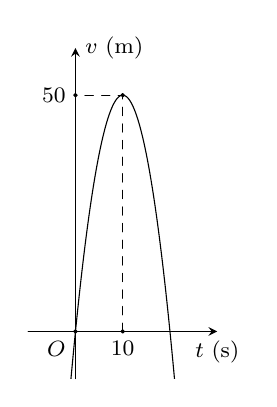
\begin{tikzpicture}[>=stealth,line join=round,line cap=round,font=\footnotesize,scale=0.6]
		\draw[->] (-1,0)--(3,0)node[below]{$t$ (s)};
		\draw[->] (0,-1)--(0,6)node[right]{$v$ (m)};
		\clip (-1,-1) rectangle (3,6);		
		\draw[smooth,samples=300]
		plot[domain=-0.5:2.5](\x,{-5*(\x)*(\x-2)});
		\draw[fill=black] (0,0) circle (1pt) node[below left]{$O$};
		\draw[fill=black] (1,0) circle (1pt) node[below]{$10$};
		\draw[fill=black] (0,5) circle (1pt) node[left]{$50$};
		\draw[fill=black] (1,5) circle (1pt);
		\draw[dashed](1,0)--(1,5)--(0,5);
		\end{tikzpicture}
	}
	\loigiai{
		Hàm vận tốc $v(t)=at^2+bt+c$ có dạng là đường Parabol có đỉnh $I(10;50)$, đồng thời đi qua gốc tọa độ $O(0;0)$, suy ra
		$\heva{&a\cdot 0^2+b\cdot 0+c=0 \\& -\dfrac{b}{2a}=10 \\& a\cdot 10^2+b\cdot 10+c=50} \Leftrightarrow \heva{&c=0 \\& 20a+b=0 \\& a\cdot 10^2+b\cdot 10+0=50} \Leftrightarrow \heva{&c=0 \\& a=-\dfrac{1}{2} \\& b=10.}$\\
		Suy ra $v(t)=-\dfrac{1}{2}t^2+10t$.\\
		Theo đồ thị thì xe bắt đầu tăng tốc lúc $t=0$ và đạt vận tốc cao nhất lúc $t=10$ s nên quãng đường đi được của xe từ lúc bắt đầu tăng tốc đến lúc đạt vận tốc cao nhất là
		$$\displaystyle\int\limits_0^{10} v(t)\mathrm{\,d}t=\displaystyle\int\limits_0^{10}\left(-\dfrac{1}{2} t^2+10t\right)\mathrm{d}t=\left(-\dfrac{1}{6} t^3+5t^2\right)\bigg|_0^{10}=\dfrac{1000}{3} \text{ m.}$$}
\end{ex}
\begin{ex}%[Dự án TLDH3-Nhóm Latex, Kiều Ngân]%[2D3K3-7]%Câu 43.
	Tốc độ phát triển của số lượng vi khuẩn trong hồ bơi được mô hình bởi hàm số $B'(t)=\dfrac{1000}{(1+0{,}25t)^2}$, $t\ge 0$, trong đó $B(t)$ là số lượng vi khuẩn trên mỗi ml nước tại ngày thứ $t$. Số lượng vi khuẩn ban đầu là $600$ con trên mỗi ml nước. Biết rằng mức độ an toàn cho người sử dụng hồ bơi là số vi khuẩn phải dưới $4000$ con trên mỗi ml nước. Hỏi sau bao nhiêu ngày thì người ta phải xử lí và thay nước mới cho hồ bơi. 
	\choice
	{\True $23$ ngày}
	{$22$ ngày}
	{$24$ ngày}
	{$25$ ngày}
	\loigiai{
		Số lượng của vi khuẩn tại ngày thứ $t$ được mô hình bởi hàm số $B(t)$ là nguyên hàm của $B’(t)$.
		$$B(t)=\displaystyle\int \dfrac{1000}{(1+0{,}25t)^2}\mathrm{\,d}t=1000\displaystyle\int(1+0{,}25t)^{-2}\mathrm{\,d}t=-\dfrac{1000}{0{,}25(1+0{,}25t)}+C.$$
		Số lượng vi khuẩn lúc ban đầu là $600$ con trên mỗi ml nước nên
		$$B(0)=600\Leftrightarrow -\dfrac{1000}{0{,}25(1+0{,}25\cdot 0)}+C=600\Leftrightarrow C=4600.$$
		Suy ra hàm số biểu thị cho số lượng vi khuẩn tại ngày thứ $t$ là
		$$B(t)=-\dfrac{1000}{0{,}25(1+0{,}25t)}+4600.$$
		Số lượng vi khuẩn dưới $4000$ con trên mỗi ml nước thì người bơi vẫn an toàn; và người bơi không an toàn khi
		\begin{eqnarray*}
			&&B(t)\ge 4000 \Leftrightarrow -\dfrac{1000}{0{,}25(1+0{,}25t)}+4600\ge 4000\\
			&\Leftrightarrow& -\dfrac{1000}{0{,}25(1+0{,}25t)}\ge -600\Leftrightarrow 1+0{,}25t\ge \dfrac{20}{3}\\
			&\Leftrightarrow& t\ge \dfrac{68}{3}\approx 22{,}67.
		\end{eqnarray*}
		Vậy sau ngày thứ $23$ thì số lượng vi khuẩn sẽ là $4000$ con và hồ bơi bắt đầu cần thay nước.}
\end{ex}
\begin{ex}%[Dự án TLDH3-Nhóm Latex, Kiều Ngân]%[2D3K3-7]%Câu 44.
	Người ta thay nước mới cho một bể bơi có dạng hình hộp chữ nhật có độ sâu là $h_1=300$ cm. Giả sử $h(t)$ là chiều cao (tính bằng cm) của mực nước bơm được tại thời điểm $t$ giây, biết rằng tốc độ tăng của chiều cao mực nước tại giây thứ $t$ là $h'(t)=\dfrac{1}{500}\sqrt[3]{t+3}$ và lúc đầu hồ bơi không có nước. Hỏi sau khoảng bao lâu thì nước bơm được $\dfrac{3}{4}$ độ sâu của hồ bơi?
	\choice
	{\True $2$ giờ $7$ phút}
	{$1$ giờ $7$ phút}
	{$4$ giờ $7$ phút}
	{$3$ giờ $7$ phút}
	\loigiai{
		Ta biết rằng chiều cao $h(t)$ của mực nước bơm được chính là nguyên hàm của tốc độ tăng $h’(t)$ của chiều cao mực nước.
		$$h(t)=\displaystyle\int h'(t)\mathrm{\,d}t=\displaystyle\int \dfrac{1}{500}\sqrt[3]{t+3}\mathrm{\,d}t=\dfrac{3}{2000}(t+3)^{\tfrac{4}{3}}+C.$$
		Lúc ban đầu (tại $t=0$) hồ bơi không chứa nước, nghĩa là
		$$h(t)=0\Leftrightarrow \dfrac{3}{2000}(0+3)^{\tfrac{4}{3}}+C=0\Leftrightarrow C=-\dfrac{3^{\tfrac{7}{3}}}{2000}.$$
		Suy ra mực nước bơm được tại thời điểm $t$ giây là
		$$h(t)=\dfrac{3}{2000}(t+3)^{\tfrac{4}{3}}-\dfrac{3^{\tfrac{7}{3}}}{2000}.$$
		Theo giả thiết, lượng nước bơm được bằng $\dfrac{3}{4}$ độ sâu của hồ bơi nên ta có
		$$h(t)=\dfrac{3}{4}h_1\Leftrightarrow \dfrac{3}{2000}(t+3)^{\tfrac{4}{3}}-\dfrac{3^{\tfrac{7}{3}}}{2000}=\dfrac{3}{4}\cdot 300 \Rightarrow t\approx 7619 \text{ s.}$$
		Vậy sau khoảng thời gian $2$ giờ $7$ phút thì bơm được $\dfrac{3}{4}$ độ sâu của hồ bơi.}
\end{ex}
\begin{ex}%[Dự án TLDH3-Nhóm Latex, Kiều Ngân]%[2D3K3-7]%Câu 45.
	Trong một đợt xả lũ, nhà máy thủy điện A đã xả lũ trong $30$ phút với tốc độ lưu lượng nước tại thời điểm $t$ giây là $v(t)=10t+500$ (m$^3$/s). Hỏi sau thời gian xả lũ trên thì hồ chứa nước của nhà máy đã thoát đi một lượng nước là bao nhiêu?
	\choice
	{\True $17{,}1$ triệu khối nước}
	{$16{,}1$ triệu khối nước}
	{$18{,}1$ triệu khối nước}
	{$19{,}1$ triệu khối nước}
	\loigiai{
		Lượng nước lũ đã xả trong khoảng thời gian $30$ phút ($1800$ giây) sẽ bằng
		$$L=\displaystyle\int\limits_0^{1800}v'(t)\mathrm{\,d}t=\displaystyle\int\limits_0^{1800}(10t+500)\mathrm{\,d}t=(5t^2+500t)\bigg|_0^{1800}=17{,}1\cdot 10^6 \text{ (m$^3$).}$$
		Vậy trong khoảng thời gian $30$ phút, nhà máy đã xả một lượng nước là $17{,}1$ triệu khối, tức là hồ chứa nước đã thoát đi $17{,}1$ triệu khối nước.}
\end{ex}
\begin{ex}%[Dự án TLDH3-Nhóm Latex, Kiều Ngân]%[2D3K3-7]%Câu 46.
	Sau $t$ giờ làm việc một người thợ có thể sản xuất với tốc độ là $q(t)=100+\mathrm{e}^{-0{,}5t}$ đơn vị sản phẩm trong $1$ giờ. Giả sử người đó bắt đầu làm việc từ lúc $7$ giờ sáng. Hỏi người đó sẽ sản xuất được bao nhiêu đơn vị sản phẩm giữa $8$ giờ sáng và $11$ giờ trưa?
	\choice
	{\True $401$ đơn vị sản phẩm}
	{$403$ đơn vị sản phẩm}
	{$601$ đơn vị sản phẩm}
	{$501$ đơn vị sản phẩm}
	\loigiai{
		Gọi $S(t)$ là số đơn vị sản phẩm mà công nhân sản xuất được sau $t$ giờ tính từ lúc $7$ giờ sáng. Ta có
		$$S'(t)=q(t)=100+\mathrm{e}^{-0{,}5t}.$$
		Số đơn vị sản phẩm người đó sản xuất được từ $8$ giờ sáng $(t=1)$ đến $11$ giờ trưa $(t=5)$ là
		$$\displaystyle\int\limits_1^5 q(t)\mathrm{\,d}t=\displaystyle\int\limits_1^5(100+\mathrm{e}^{-0{,}5t})\mathrm{\,d}t\approx 401\text{ đơn vị sản phẩm.}$$
	}
\end{ex}
\begin{ex}%[Dự án TLDH3-Nhóm Latex, Kiều Ngân]%[2D3K3-5]%Câu 47.
	\immini{
		Một khối cầu có bán kính $5$ dm, người ta cắt bỏ $2$ phần bằng $2$ mặt phẳng vuông góc bán kính và cách tâm $3$ dm để làm một chiếc lu đựng (như hình vẽ). Thể tích của cái lu là 
		\choice
		{\True $132\pi$ (dm$^3$)}
		{$41\pi$ (dm$^3$)}
		{$\dfrac{100\pi }{3}$ (dm$^3$)}
		{$43\pi$ (dm$^3$)}
	}{
		\begin{tikzpicture}[>=stealth,line join=round,line cap=round,font=\footnotesize,scale=0.5]
		\draw[name path=c] (0,0) circle (5 cm);
		\draw[dashed] (4,3) arc (0:180:4 cm and 0.7 cm);
		\draw (4,3) arc (0:-180:4 cm and 0.7 cm);
		\draw[dashed] (4,-3) arc (0:180:4 cm and 0.7 cm);
		\draw (4,-3) arc (0:-180:4 cm and 0.7 cm);
		\draw[dashed](0,-5)--(0,5) (0,0)--(5,0);
		\draw[color=black] (0,-5)circle(1pt);
		\draw[color=black] (0,-3)circle(1pt);
		\draw[color=black] (0,3)circle(1pt);
		\draw[color=black] (0,5)circle(1pt);
		\draw[color=black] (5,0)circle(1pt);
		\node [above]at (2.5,0){$5$ dm};
		\node [left]at (0,1){$3$ dm};
		\node [left]at (0,-1){$3$ dm};
		\end{tikzpicture}
	}
	\loigiai{
		\immini{
			Xét đường cong cạnh bên của cái lu là đường cong $AC$ và chọn hệ trục tọa độ $Oxy$ như hình vẽ.\\
			Ta có phương trình đường $BC\colon y=\sqrt{25-x^2}\ge 0$.\\
			Khi đó thể tích của cái lu chính là
			$$V_{\text{lu}}=2\pi \displaystyle\int\limits_0^3\left(\sqrt{25-x^2}\right)^2\mathrm{\,d}x=132\pi\text{ (dm$^3$)}.$$
		}{
			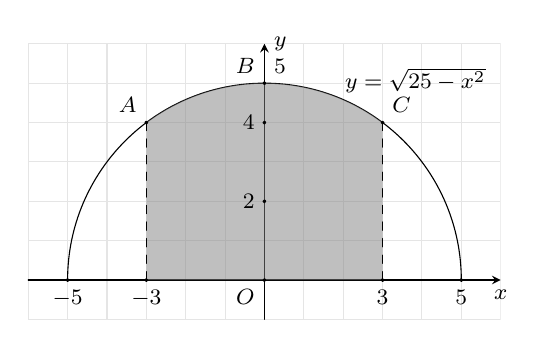
\begin{tikzpicture}[>=stealth,line join=round,line cap=round,font=\footnotesize,scale=0.5]
			\draw[->] (-6,0)--(6,0)node[below]{$x$};
			\draw[->] (0,-1)--(0,6)node[right]{$y$};
			\clip (-6,-1) rectangle (6,6);
			\draw [opacity=0.1](-6,-1) grid (6,6);		
			\draw (5,0) arc(0:180:5cm and 5cm);
			\fill[gray, opacity=0.5] 
			plot[domain=-3:3](\x,{sqrt(25-(\x)^2)})--(3,0)--(-3,0)--cycle;
			\draw[fill=black] (0,0) circle (1pt) node[below left]{$O$};
			\draw[fill=black] (3,0) circle (1pt) node[below]{$3$};
			\draw[fill=black] (5,0) circle (1pt) node[below]{$5$};
			\draw[fill=black] (-3,0) circle (1pt) node[below]{$-3$};
			\draw[fill=black] (-5,0) circle (1pt) node[below]{$-5$};
			\draw[fill=black] (0,2) circle (1pt) node[left]{$2$};
			\draw[fill=black] (0,4) circle (1pt) node[left]{$4$};
			\draw[fill=black] (0,5) circle (1pt) node[above right]{$5$} node[above left]{$B$};
			\draw[fill=black] (-3,4) circle (1pt) node[above left]{$A$};
			\draw[fill=black] (3,4) circle (1pt) node[above right]{$C$};
			\draw[fill=black] (1.8,4.5) node[above right]{$y=\sqrt{25-x^2}$};
			\draw[dashed](3,0)--(3,4) (-3,0)--(-3,4);
			\end{tikzpicture}
		}
	}
\end{ex}
\begin{ex}%[Dự án TLDH3-Nhóm Latex, Kiều Ngân]%[2D3K3-5]%Câu 48.
	\immini{
		Một cái nêm được tạo thành bằng cách cắt ra từ một khúc gỗ hình trụ có bán kính bằng $4$ (cm) bởi hai mặt phẳng gồm mặt phẳng thứ nhất vuông góc với trục của hình trụ, mặt phẳng thứ hai cắt mặt phẳng thứ nhất dọc theo một đường kính của hình trụ và góc giữa hai mặt phẳng đó bằng $30^\circ$. Tính thể tích cái nêm đó?
		\choice
		{$\dfrac{64\sqrt{3}}{9}$ (cm$^3$)}
		{$\dfrac{128\pi \sqrt{3}}{9}$ (cm$^3$)}
		{\True $\dfrac{128\sqrt{3}}{9}$ (cm$^3$)}
		{$\dfrac{64\pi \sqrt{3}}{9}$ (cm$^3$)}
	}{
		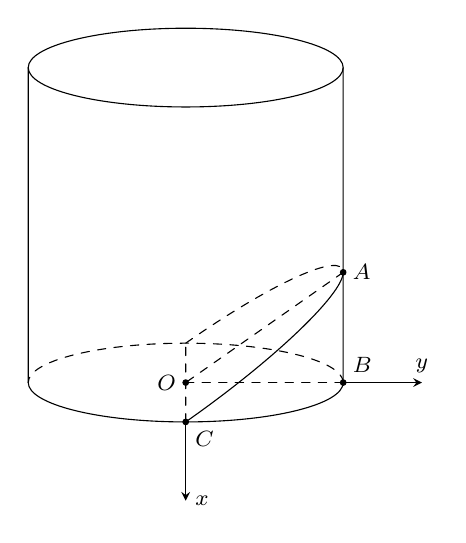
\begin{tikzpicture}[>=stealth,line join=round,line cap=round,font=\footnotesize,scale=1]
		\draw[dashed] (2,0)--(0,0);
		\draw[dashed] (2,0) arc(0:180:2cm and 0.5cm);
		\draw (2,0) arc(0:-180:2cm and 0.5cm)--(-2,4);
		\draw (-2,4) arc(-180:180:2cm and 0.5cm);
		\draw[dashed,yslant=.7] (0,0.5) arc(90:0:2cm and 0.5cm) coordinate (A);
		\draw[yslant=.7] (0,-0.5) arc(-90:0:2cm and 0.5cm);
		\draw (2,4)--(A)--(2,0);
		\draw[dashed] (A)--(0,0) (0,-0.5)--(0,0.5);
		\draw[->](2,0)--(3,0) node[above]{$y$};
		\draw[->](0,-0.5)--(0,-1.5) node[right]{$x$};
		\draw[fill=black](0,0) coordinate (O) circle(1pt) node[left]{$O$};
		\draw[fill=black] (2,0) coordinate (B) circle(1pt) node[above right]{$B$};
		\draw[fill=black] (A) circle(1pt) node[right]{$A$};
		\draw[fill=black] (0,-0.5) circle(1pt) node[below right]{$C$};
		\tkzMarkAngle(B,O,A)
		\end{tikzpicture}
	}
	\loigiai{
		Gắn mặt phẳng tọa độ $Oxy$ trùng với mặt cắt vuông góc với trục hình trụ.\\
		Ta có $OB=4$, $\widehat{AOB}=30^\circ$.\\
		Gọi $S(x)$ là diện tích thiết diện của cái nêm cắt bởi mặt phẳng vuông góc với trục $Ox$ tại điểm có hoành độ bằng $x$.\\
		Cụ thể $S(x)$ là diện tích của các tam giác vuông tại đỉnh thuộc cung $BC$ với $C(4,0)$.\\
		Do đó $S(x)=\dfrac{1}{2}\sqrt{16-x^2}\sqrt{16-x^2}\tan 30^{\circ}=\dfrac{16-x^2}{2\sqrt{3}}$.\\
		Khi đó thể tích của cái nêm bằng $V=2\displaystyle\int\limits_0^4 S(x)\mathrm{\,d}x=\dfrac{1}{\sqrt{3}}\displaystyle\int\limits_0^4\left(16-x^2\right)\mathrm{d}x=\dfrac{128\sqrt{3}}{9}\left(\mathrm{cm}^3\right)$.}
\end{ex}
\begin{ex}%[Dự án TLDH3-Nhóm Latex, Kiều Ngân]%[2D3K3-5]%Câu 49.
	Một cái nêm được tạo thành bằng cách cắt ra từ một khúc gỗ hình trụ có bán kính bằng $1$ m bởi hai mặt phẳng gồm mặt phẳng thứ nhất vuông góc với trục của hình trụ, mặt phẳng thứ hai cắt mặt phẳng thứ nhất dọc theo một đường kính của hình trụ và góc giữa hai mặt phẳng đó bằng $45^\circ$. Tính thể tích cái nêm đó. 
	\choice
	{$\dfrac{1}{3}$ m$^3$}
	{\True $\dfrac{2}{3}$ m$^3$}
	{$\dfrac{1}{4}$ m$^3$}
	{$\dfrac{1}{2}$ m$^3$}
	\loigiai{
		Gắn mặt phẳng tọa độ $Oxy$ trùng với mặt cắt vuông góc với trục hình trụ.\\
		Ta có $OB=1$, $\widehat{AOB}=45^\circ$.\\
		Gọi $S(x)$ là diện tích thiết diện của cái nêm cắt bởi mặt phẳng vuông góc với trục $Ox$ tại điểm có hoành độ bằng $x$.\\
		Cụ thể $S(x)$ là diện tích của các tam giác vuông tại đỉnh thuộc cung $BC$ với $C(1,0)$.\\
		Do đó $S(x)=\dfrac{1}{2}\sqrt{1-x^2}\sqrt{1-x^2}\tan 45^{\circ}=\dfrac{1-x^2}{2}$.\\
		Khi đó thể tích của cái nêm bằng $V=2\displaystyle\int\limits_0^1 S(x)\mathrm{\,d}x=\displaystyle\int\limits_0^1\left(1-x^2\right)\mathrm{d}x=\dfrac{2}{3}$ (cm$^3$).}
\end{ex}
\begin{ex}%[Dự án TLDH3-Nhóm Latex, Kiều Ngân]%[2D3K3-5]%Câu 50.
	\immini{
		Từ một khúc gỗ hình trụ có đường kính $30$ cm, người ta cắt khúc gỗ bởi một mặt phẳng đi qua đường kính đáy và nghiêng với đáy một góc $45^\circ$ để lấy một hình nêm (xem hình minh họa dưới đây). Kí hiệu $V$ là thể tích của hình nêm (hình 2). Tính thể tích của $V$. 
		\choice
		{\True $V=2250$ (cm$^3$)}
		{$V=\dfrac{225\pi }{4}$ (cm$^3$)}
		{$V=1250$ (cm$^3$)}
		{$V=1350$ (cm$^3$)}
	}{
		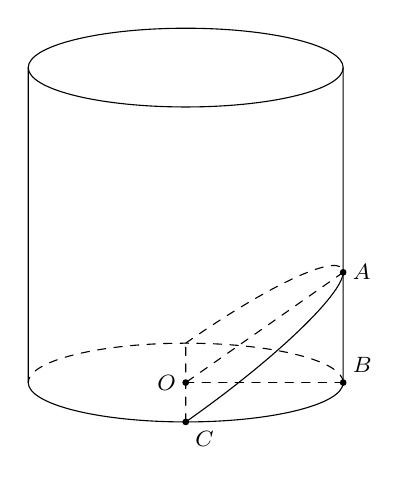
\begin{tikzpicture}[>=stealth,line join=round,line cap=round,font=\footnotesize,scale=1]
		\draw[dashed] (2,0)--(0,0);
		\draw[dashed] (2,0) arc(0:180:2cm and 0.5cm);
		\draw (2,0) arc(0:-180:2cm and 0.5cm)--(-2,4);
		\draw (-2,4) arc(-180:180:2cm and 0.5cm);
		\draw[dashed,yslant=.7] (0,0.5) arc(90:0:2cm and 0.5cm) coordinate (A);
		\draw[yslant=.7] (0,-0.5) arc(-90:0:2cm and 0.5cm);
		\draw (2,4)--(A)--(2,0);
		\draw[dashed] (A)--(0,0) (0,-0.5)--(0,0.5);
		\draw[fill=black](0,0) coordinate (O) circle(1pt) node[left]{$O$};
		\draw[fill=black] (2,0) coordinate (B) circle(1pt) node[above right]{$B$};
		\draw[fill=black] (A) circle(1pt) node[right]{$A$};
		\draw[fill=black] (0,-0.5) circle(1pt) node[below right]{$C$};
		\tkzMarkAngle(B,O,A)
		\end{tikzpicture}
		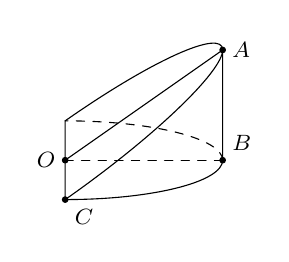
\begin{tikzpicture}[>=stealth,line join=round,line cap=round,font=\footnotesize,scale=1]
		\draw [dashed](2,0)--(0,0);
		\draw[dashed] (2,0) arc(0:90:2cm and 0.5cm);
		\draw (2,0) arc(0:-90:2cm and 0.5cm);
		\draw[yslant=.7] (0,0.5) arc(90:0:2cm and 0.5cm) coordinate (A);
		\draw[yslant=.7] (0,-0.5) arc(-90:0:2cm and 0.5cm);
		\draw (A)--(2,0);
		\draw (A)--(0,0) (0,-0.5)--(0,0.5);
		\draw[fill=black](0,0) coordinate (O) circle(1pt) node[left]{$O$};
		\draw[fill=black] (2,0) coordinate (B) circle(1pt) node[above right]{$B$};
		\draw[fill=black] (A) circle(1pt) node[right]{$A$};
		\draw[fill=black] (0,-0.5) circle(1pt) node[below right]{$C$};
		\tkzMarkAngle(B,O,A)
		\end{tikzpicture}
	}
	\loigiai{
		\immini{
			Gắn mặt phẳng tọa độ $Oxy$ trùng với mặt cắt vuông góc với trục hình trụ.\\
			Ta có $OB=15$, $\widehat{AOB}=45^\circ$.\\
			Gọi $S(x)$ là diện tích thiết diện của cái nêm cắt bởi mặt phẳng vuông góc với trục $Ox$ tại điểm có hoành độ bằng $x$.\\
			Cụ thể $S(x)$ là diện tích của các tam giác vuông tại đỉnh thuộc cung $BC$ với $C(15,0)$.\\
			Do đó $S(x)=\dfrac{1}{2}\sqrt{15^2-x^2}\sqrt{15^2-x^2}\tan 45^{\circ}=\dfrac{15^2-x^2}{2}$.\\
			Khi đó thể tích của cái nêm bằng $$V=2\displaystyle\int\limits_0^{15} S(x)\mathrm{\,d}x=\displaystyle\int\limits_0^{15}\left(15^2-x^2\right)\mathrm{\,d}x=2250\text{ (cm$^3$).}$$
		}{
			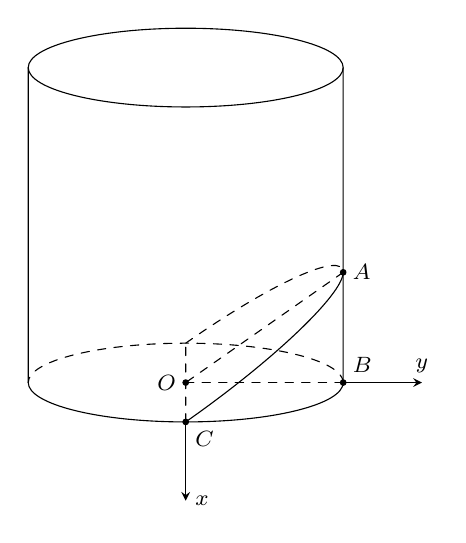
\begin{tikzpicture}[>=stealth,line join=round,line cap=round,font=\footnotesize,scale=1]
			\draw[dashed] (2,0)--(0,0);
			\draw[dashed] (2,0) arc(0:180:2cm and 0.5cm);
			\draw (2,0) arc(0:-180:2cm and 0.5cm)--(-2,4);
			\draw (-2,4) arc(-180:180:2cm and 0.5cm);
			\draw[dashed,yslant=.7] (0,0.5) arc(90:0:2cm and 0.5cm) coordinate (A);
			\draw[yslant=.7] (0,-0.5) arc(-90:0:2cm and 0.5cm);
			\draw (2,4)--(A)--(2,0);
			\draw[dashed] (A)--(0,0) (0,-0.5)--(0,0.5);
			\draw[->](2,0)--(3,0) node[above]{$y$};
			\draw[->](0,-0.5)--(0,-1.5) node[right]{$x$};
			\draw[fill=black](0,0) coordinate (O) circle(1pt) node[left]{$O$};
			\draw[fill=black] (2,0) coordinate (B) circle(1pt) node[above right]{$B$};
			\draw[fill=black] (A) circle(1pt) node[right]{$A$};
			\draw[fill=black] (0,-0.5) circle(1pt) node[below right]{$C$};
			\tkzMarkAngle(B,O,A)
			\end{tikzpicture}
		}
	}
\end{ex}
\Closesolutionfile{ans}
% \DAPAN
\inputansbox{10}{ans/ansCD2D3-3.1-2}

